\documentclass[12pt,oneside]{book}
\pagestyle{headings}

% Note that the line below could be modified to suit a
% particular system since the "geometry" package behaves
% differently in Unix, Windows and Mac, especially for the
% top margins.
% Adjust the parameter "top" (measuring the height of the
% space allocated to a header) and "headsep" (measuring
% the distance from the bottom of the header to the
% first line of text.
\usepackage[top=1.3in,left=1.5in,bottom=1in,right=1in,headsep=0.5in]{geometry}

\usepackage{setspace}
\onehalfspacing
%\doublespacing

% Headers and footers for thesis
\usepackage{fancyhdr}

\markboth{}{}
\newcommand\startchapter[1]{\chapter{#1}\thispagestyle{myheadings}}
\newcommand\startappendix[1]{\chapter{#1}\thispagestyle{myheadings}}
\newcommand\startfirstchapter[1]{\chapter{#1}}

% Manual addition of section to Table of Contents
\newcommand\TOCadd[1]{\newpage\phantomsection\addcontentsline{toc}{chapter}{#1}}

% Float Customization
\renewcommand{\floatpagefraction}{0.01}

% Customization of Tables of Contents and List of Figures/Tables
\usepackage{tocloft}
\renewcommand\cfttabpresnum{Table\ }
\renewcommand\cfttabnumwidth{0.75in}
\renewcommand\cftfigpresnum{Figure\ }
\renewcommand\cftfignumwidth{0.80in}
\newcommand{\HRule}{\rule{\linewidth}{0.5mm}}

% Long Table and decimal aligned columns
\usepackage{dcolumn}
\usepackage{longtable}

% Mathematics support
\usepackage{amsmath}
\usepackage{amsthm}
\usepackage{amssymb}


% Text Control
\usepackage{xspace}
\usepackage{textcase}

% Graphics
\usepackage{wasysym}
\usepackage{graphics}
\usepackage{graphicx}   % A package to allow insertion of
                        % external image files


\bibliographystyle{apalike}

\usepackage{natbib}
\usepackage{pdfpages}
\usepackage{siunitx}
\usepackage{graphicx}
\usepackage{float}
\usepackage{verbatim}
\usepackage{setspace}
\usepackage[export]{adjustbox}
\usepackage{setspace}



\begin{document}



\input frontmatter/fm


% Front Matter




\newpage

\startfirstchapter{Introduction to eDNA}
\label{chapter:introduction}





\hspace{4mm} 

The rapid and unfortunate decline in the Earth\textsc{\char13}s biodiversity is a clear and major obstacle facing humanity in the 21st century. Although this fact is widely accepted among the scientific community, the solution on how to combat this decline is still not known. One thing that is clear, however, is that researchers must expand and improve knowledge on the current state and distribution of biodiversity worldwide. In order to make informed and critical decisions regarding biodiversity, researchers must first monitor and model reliable distribution patterns, as well as estimate population sizes. Historically, this monitoring has involved invasive surveys that may even compound the issue of decline, especially when studying endangered or rare species. For this reason, it is critical that non-invasive, large scale biodiversity monitoring techniques are developed \citep{ednamonitoring}.


\vspace{5mm}


One such non-invasive technique for the monitoring of biodiversity involves the study and collection of environmental DNA. Environmental DNA, or eDNA, is mitochondrial or nuclear DNA that is released from an organism as it interacts with its environment.  Common sources of eDNA include shed skin cells, hair, blood, urine and mucous \citep{forestry}. Shed DNA can be collected by researchers for analysis. There are numerous methods in which eDNA is collected and analyzed, such as from samples of lake water \citep{goby} or other aquatic sources \citep{mussels}. eDNA has also been obtained from non-aquatic environments such as from snow, ice, or from soil \citep{soil}.

\newpage

 New and emerging technology has advanced researchers\textsc{\char13} ability to collect and analyze this shed eDNA. In particular, studies of eDNA have assisted scientists in detecting the extant of a species in a certain area and have facilitated conservation efforts \citep{speciesDetection,limitations}. Most commonly, environmental DNA is analyzed via DNA sequencing methods such as metagenomics and qPCR \citep{geneexpression}.



\vspace{5mm}




The analysis of eDNA allows researchers to study species without the capture of the target organism. This is of benefit in particular for species that are endangered and allows researchers to conduct investigations with minimal environmental disruption. Before the common usage of eDNA, methods for studying aquatic diversity included fishing and trapping. These invasive methods are expensive, time consuming and directly impact the habitat in which the researcher is studying. Indeed, using classical sampling methods to study fish may negatively impact the species and environment (especially electrofishing) \citep{electrofishing,freshwaterbiodiversity}. Collection and study of eDNA however, is non-invasive and only requires minimal sampling.\citep{ednaPH,streamdwelling}. Analysis of environmental DNA has already been used successfully as a surveillance method for rare fish species \citep{rareaquatic}.


\vspace{5mm}

The ability to sequence miniscule concentrations of eDNA directly from aquatic environments is revolutionizing the field of ecological monitoring and management \citep{MarineSystems}. Although most studies regarding eDNA in aquatic environments have focused on freshwater, eDNA is increasingly being used to study ocean and marine systems.  Corporations involved with aquatic conservation and fisheries management are progressively incorporating eDNA into their business and research \citep{usesofedna}. Hence, it is critical that researchers understand the physical and chemical properties of eDNA, such as degradation or the impact of ecological covariates. The research we present in this thesis has the potential to be of particular use for those interested in fisheries monitoring. 


   \vspace{4mm}


One species that researchers have studied using eDNA methodology is the invasive American signal crayfish, \textit{Pacifastacus leniusculuscray}. This crayfish is problematic and is the current leading cause of decline among UK\textsc{\char13}s native crayfish species. The practice of eDNA related techniques allows for non-invasive and potentially early detection of these crayfish \textit{Pacifastacus leniusculuscray}. Early detection of eDNA may allow for their eradication before the levels are large enough to detect manually and before it is too late to act \citep{crayfish}.

    
\vspace{5mm}


Researchers have also used eDNA to study the Coastal tailed frog (\textit{Ascaphus truei}). By using eDNA and testing water samples at a variety of lakes and watersheds, researchers were able to expand knowledge of known Coastal tailed frog distributions in British Columbia \citep{forestry}.

    \vspace{5mm}

The association between eDNA concentration and species abundance is the subject of ongoing study. Research of native fish populations have shown that studying eDNA concentration in water samples may be able to predict fish abundance as well as, or better than more invasive and costly methods \citep{fishabundance,salmonabundance}. Moreover, an ever-increasing number of non-invasive eDNA techniques produce reliable enough DNA to address nearly all questions that could be obtained via traditional methods \citep{ecounderstanding}.
\vspace{5mm}

In Florida, researchers collected eDNA to study the abundance and occupancy of invasive Burmese Pythons, \textit{Python molurus bivitatus}, in the Everglades \citep{pythons}. These pythons pose significant threats to native species.  Burmese Pythons are considered to  be largely mysterious and their population distribution in the Florida area is not well documented. These pythons mainly reside within inaccessible habitats, making standard sampling nearly impossible. Because they are so evasive, only a single study with the goal of estimating detection probability has been conducted in which standard sampling techniques were attempted \citep{standardPython}.  This standard study did not have very promising results and had very few sightings of the pythons. However, researchers using eDNA sampling were able to extensively expand knowledge of the python distribution via studies done on water samples taken throughout the Everglades. 

 \vspace{5mm}
Overall, the study and analysis of environmental DNA is an emerging method of science that has been used successfully for the detection and study of rare species. The less invasive methods utilized while studying eDNA are becoming increasingly important as biodiversity continues to decline worldwide \citep{GreenSturgeon}.

\vspace{5mm}

 In Chapter 2 of this thesis, we introduce the preliminary content that is needed to understand the experiments. This includes a survey of methods used to analyze eDNA, and a summary of past research on the topic of eDNA. In Chapter 3 of this thesis, we use water samples from tanks in which the biomass of Coho is known to study the relationship between eDNA concentration and biomass \citep{fishforensics}. In Chapter 4, we extend this result by considering the impact of flow or dilution on eDNA. The experiments in Chapters 3 and 4 were conducted by Jeff MacAdams in collaboration with EcoFish Research. In Chapter 5, we bridge the gap to the field, where we build models for predicting Coho biomass using eDNA concentrations and several environmental covariates (collected by EcoFish personnel). Finally, in Chapter 6 we provide a summary of the thesis and present our conclusions.






\startchapter{Statistical Methods}
\label{chapter:problem}


\newlength{\savedunitlength}
\setlength{\unitlength}{2em}


\section{Summary of qPCR}

Real time PCR or quantitative polymerase chain reaction (`qPCR') is a well-established laboratory technique that allows for the real time detection and quantification of microbial DNA \citep{introqpcr}.



\begin{figure}[H]
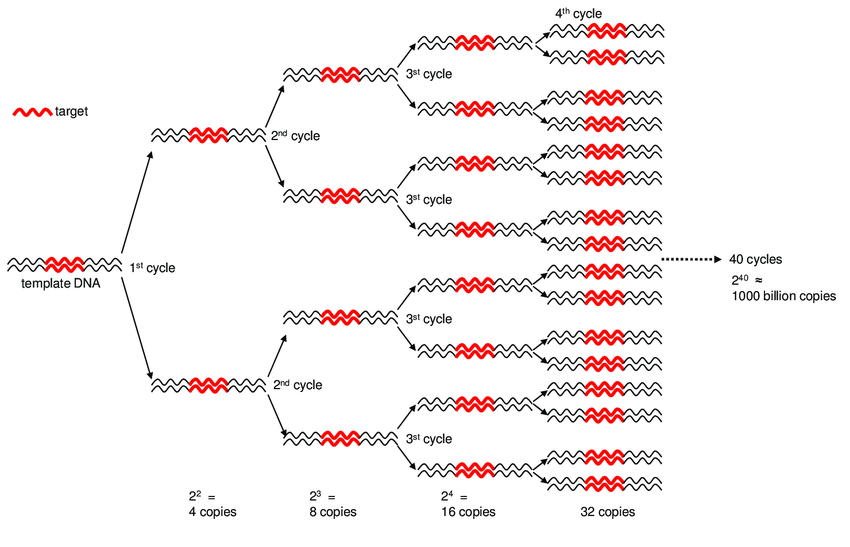
\includegraphics[scale=0.5]{Chapter2Images/amp.png}
\caption{Assuming that the qPCR runs with perfect efficiency, we expect to see a doubling of DNA after every cycle \citep{foodscience}.}
\label{fig:amp}
\end{figure} 

\newpage



Figure~\ref{fig:amp} is a basic visualization of how qPCR works. At each cycle, assuming perfect efficiency, the amount of target DNA should double.

\vspace{5mm}

To measure concentration of DNA, a fluorometer detects levels of fluorescence as the thermal cycler runs, and the level of fluorescent signal reflects the amount of target DNA in the sample. During the first cycles, the amount of fluorescence produced is not significant enough to separate from background light. As the experiment progresses, the fluorescent signal may increase above a certain detectable level (corresponding to the initial number of template DNA). This point is known as the `Quantification Cycle' or the Cycle Threshold (CT). This value allows for the detection and quantification of target DNA \citep{ctmethod}. Typically, a specified number of cycles is decided on as a `cutoff' value. That is, if we have gone through a specified number of cycles, and still have not detected a signal, we would consider this to be indicative that the target DNA was not present in the sample.









\vspace{5mm}


In other words, as the experiment progresses, fluorescence is observed when the specified target DNA is detected. If it only takes a few cycles, this results in a low Cycle Threshold (`CT') score and indicates high levels of target DNA were present in the sample. The more cycles it takes to detect a visible fluorescence signal, the higher the CT score, indicating that less of the target DNA is present in the sample \citep{dropletqpcr,independentreplicates}.

\vspace{5mm}

Another concept that is often used when discussing eDNA related studies is the `Limit of Detection' or `LoD'. With respect to eDNA studies, the `LoD' is defined as the minimum amount of target DNA required to conclude with high probability that specified target DNA exists in the sample. Researchers often agree upon a CT value to determine a LoD. For example, in our later research we define the LoD to be CT $<$ 50. Hence, if there is still no visible fluorescence after 50 cycles (i.e. CT $>$50), we conclude that the sample does not contain the target DNA. In other cases, LoD may be defined in terms of the number of copies of target DNA.

\newpage

\section{Biomass and eDNA concentration}

The study by \cite{biomass} deals directly with estimation of fish biomass from eDNA concentration and helps to illustrate how statistical analysis is performed on eDNA data.

\vspace{5mm}

In this study, researchers hypothesized that eDNA released from the common carp, \textit{Cyprinus carpio} is positively correlated with the carp's biomass. Furthermore, researchers extended their knowledge of eDNA to study carp in the field, where they incorporated several environmental covariates into their statistical models.

\vspace{5mm}

To study collected samples of carp eDNA, researchers used a carp specific mitochondrial gene fragment. To construct the standard curve, qPCR was conducted on the target species using a pGEM-T Easy Vector, and a dilution series of the carp DNA containing 30 to 30,000 copies of DNA was created. This involved plotting the absorbance obtained using known concentrations of carp DNA. Using the standard curve for carp, researchers were able to obtain estimates for the number of copies of carp DNA in each sample they ran. Water that was collected as samples was immediately filtered using a centrifuge. 

\vspace{5mm}

Since one copy of carp DNA was detected in each triplicate, the Limit of Detection (LoD) for carp DNA was chosen to be a detection of at least one copy of carp specific DNA. Three technical replicates (sub samples from the same triplicate) were run on each sample and if a technical replicate showed a negative result, it was assigned a value of zero. The mean value obtained in the three replicates was the quantity chosen to be used in regression. In addition, three wells containing no carp DNA were used as negative controls. In each of the three wells chosen to be negative controls, no eDNA of carp was detected.

\vspace{5mm}

The first experiment was done using tanks. Juvenile carp in the Mie Prefecture of Japan were captured and transferred to a lab in Kyoto.
To study the impact of biomass, twelve tanks were used.  Four tanks had only one carp, four tanks had five carps and the other four tanks contained ten carps. The water temperature was kept constant among the separate tanks. On the sixth day, triplicate samples of 50mL were collected from each tank. 







\begin{figure}[H]
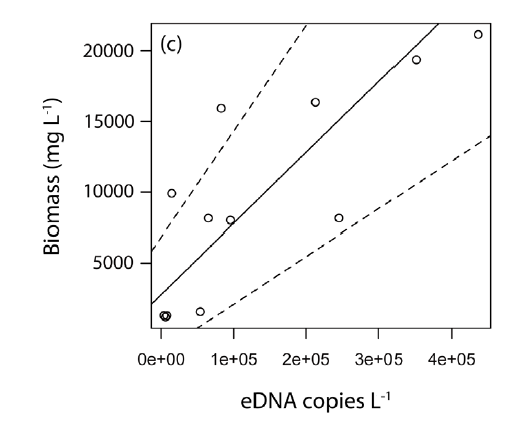
\includegraphics{Chapter2Images/eDNAcopies.png} 
\caption{This figure is a plot of data obtained of biomass concentration (y-axis) versus eDNA copies per Litre (x-axis). There was a
significant positive correlation between the number of eDNA
copies and carp biomass per 1 L (y = 0.050x+2789, $R^{2}$ =0.66,
p= 0.001). There are twelve points, one for each tank used in the tank experiment. There is an overlapping of three points in the bottom left hand side of the figure
 \citep{biomass}.}
\label{fig:copies}
\end{figure}


  Figure~\ref{fig:copies} shows the result of linear regression applied to the qPCR data. Using linear regression, researchers were able to obtain estimates of coefficients and estimates of standard errors. In this experiment, linear regression was able to provide an adequate analysis with moderate explanatory power. The $R^{2}=0.66$ indicates that this linear model does a moderate job in explaining the variance in the data. The dashed lines show the associated confidence bands for the regression estimate. We also show later in our analysis that linear regression can be used as a reliable method for obtaining estimates of Coho biomass. 


\vspace{5mm}

To bridge the research into the field, researchers collected water samples from Lake Biwa in Japan. The area of the lake in which they sampled was known to be inhabited by the common carp. From 21 distinct sites on the lake, 2-L samples of water were collected. Moreover, several environmental covariates were recorded such as water temperature, conductivity, etc. The samples were immediately transferred  back to the lab where they were extracted and analyzed using the same standard curve for carp. All sequences from which the eDNA analysis indicated presence of carp, were confirmed to be regions of the lake that did contain carp.


\vspace{5mm}

 In this experiment, researchers made use of General Linear Models and Stepwise selection. By comparing $R^{2}$ values, researchers were able to make conclusions regarding which covariates should be included in models. The model that included water temperature as a covariate turned out to work best in the field experiment and several environmental covariates such as pH or chlorophyll were seen to not be significant.


\begin{figure}[H]
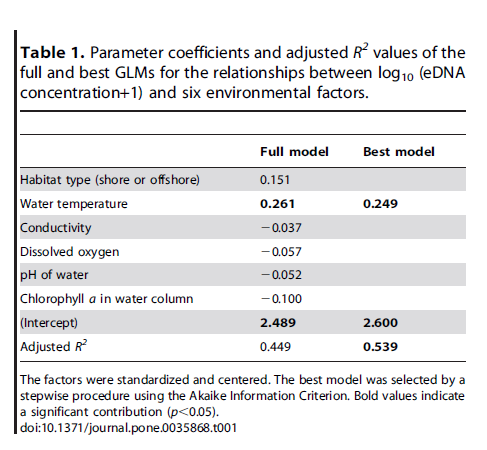
\includegraphics{Chapter2Images/biomassGLM.png} 
\caption{ Table summarizing the various estimates and adjusted $R^{2}$ values for a full model and the best model.
 \citep{biomass}.}
\label{fig:glm}
\end{figure}

\newpage

 Figure~\ref{fig:glm} summarizes the result of the general linear model that researchers created to evaluate the relationship between eDNA concentration and several environmental covariates. The full model contains all the above environmental covariates and has an adjusted $R^{2}$=0.449. On the other hand, the best model only contains an intercept and water temperature, and the adjusted $R^{2}$ is improved to 0.539.

\vspace{5mm}

Prior to fitting a general linear model, researchers used a variance inflation factor (VIF) to assess whether there was collinearity among the covariates. This was done by dividing the variance estimates of the full model by the variance estimates of a model that only included one term at a time. Calculating the VIF for each covariate indicated that there was not sufficient evidence to conclude that collinearity existed among any of the covariates (this was done by ensuring that the VIF was not too large, in particular, less than a common cutoff value of 5 for all covariates). The eDNA estimates were obtained as above using qPCR and comparison to the standard curve, and a log10 transformation was applied to the estimates in an effort to normalize the results. A Shapiro Wilks test applied to the residuals confirmed normality of the estimates at a 95 percent confidence level.  To select the best GLM, researchers compared models using stepwise selection based on AIC criteria. In this case, the best general linear model included the temperature of the water as an environmental covariate. Moreover, the estimate for water temperature was  significantly positive.

\vspace{5mm}

In Chapter 5, we also use a stepwise selection approach to determine which environmental covariates to include in our field models.







\section{eDNA and Species Occupancy}
 
The study by \cite{parasite} further helps to illustrate the methods in which eDNA can be used to make inference regarding target organism occupancy. The \textit{Schistocephalus solidus}-threespine stickleback pair is a commonly researched parasite/host pair. \textit{Schistocephalus solidus} is a parasitic flatworm, while the abdominal cavity of the  \textit{Gasterosteus aculeatus} (threespine stickleback) is one possible host location for this parasite. Conventional  methods for detecting if a stickleback is infected with the parasite is by simple visual detection. However, this results in not identifying parasites that are too small or have not yet grown to full size (past a certain mass threshold). 


\vspace{5mm}

An alternative, non-invasive method to detect the parasitic tapeworm involves using qPCR to test for the presence of \textit{Schistocephalus solidus} eDNA. Researchers took samples from the abdominal cavity of sticklebacks and performed qPCR to test for \textit{Schistocephalus solidus} DNA. Using this method, scientists were able to correctly assign the status to 98 percent of n=151 fish.
Moreover, not only did qPCR allow for the detection, but it also allowed for a comparative quantification of eDNA. That is, researchers were able to get an idea of how large the parasite was simply based on the results of the qPCR. Lower CT scores indicated higher presence of eDNA and was correlated with larger parasite mass. 

\vspace{6mm}

Researchers used minnow traps in Lac Temiscouata and Isle-Vertes (Quebec, Canada) to capture the sticklebacks. The fish were transferred to Laval University where they were maintained according to their natural requirements. In total, 96 fish were sampled from Lac Temiscoutata and 55 were sampled from Isle-Vertes. By the time the experiment began, all fish were considered to be adult fish. The fish were each subsequently isolated into 2 L tanks in the lab.

\vspace{5mm}

The fish were removed individually and placed on sponges. A small 1ml volume syringe filled with 100 $\mu L$ of a phosphate buffer was injected into the abdominal cavity of the fish. Without removing the needle, the syringe was pulled back until it had 100  $\mu L$ of the recently injected buffer back in the needle. The needle was then removed, and the fish was returned to its tank. This removed liquid was added directly to a tube containing 700 $\mu L$ of  Longmire Lysis preservation buffer. This was done once per day for each fish on two consecutive days. The samples were then stored in an appropriate environment to maintain the delicate structure of the DNA. Note that on the second sample, the phosphate buffer was added to the same tube containing the 700$ \mu L$ of lysis buffer from the previous day. Hence, each tube had up to 900 $\mu L$ of liquid.
Once the fish had been sampled twice, they were killed with an injection of MS-222 and dissected. Fish size, sex and mass were recorded as well as the mass and number of any  \textit{Schistocephalus solidus} parasites in the fish. A `PI' value was calculated where PI= [total mass of parasite (mg) / total mass of host plus parasite (mg)]x100.


\vspace{5mm}

To detect DNA from the parasite, researchers used a pair of primers that amplified a specific sequence from a nuclear gene in the \textit{Schistocephalus solidus} genome. The specific gene sequence has no known analogs in other species. PCR assays were then tested on genomic DNA to confirm that the primers indeed amplified the parasite DNA and did not falsely amplify other DNA from the stickleback.

\vspace{6mm}

Prior to the experiment, researchers obtained what is known as a `Standard Curve' for \textit{S.solidus} genomic DNA. A `Standard Curve', also known as a `Calibration Curve' allows researchers to make inference about DNA concentrations using previous knowledge of that species DNA \citep{standardCurve}. In this case, researchers used known concentrations of \textit{S. solidus} DNA obtained from three individuals and prepared a wide range of dilutions. At the low end, researchers prepared a 0.01 ng $\mu L^{-1}$ sample and at the high end a 0.9 ng$ \mu L^{-1}$ sample. Researchers also created multiple samples with known concentrations in between the minimum and maximum values. These solutions are referred to as the `standard solutions'.  The fluorescence produced by cycling these standard solutions was then measured using a spectrophotometer and the results were recorded. A graph was produced showing the relation between concentration of eDNA and the CT value. This is known as a `Standard Curve'.  Hence, the Standard curve allowed researchers to make conclusions about new DNA concentrations using prior knowledge of the properties of that specific target DNA. 

\vspace{5mm}

Finally, researchers were able to begin to analyze the eDNA. The removed eDNA was amplified using qPCR and the primers described. CT values were recorded when the fluorescence reached a certain threshold. Researchers included negative controls (no DNA and no primers) in each plate. Each reaction was done in triplicate. 

\vspace{5mm}

 Once the qPCR amplification had taken place, the presence or absence of eDNA in the fish was determined by comparing the obtained CT values with the standard curve. If more than 70 cycles of qPCR were needed, this was considered to be `undetermined' for the presence of parasite eDNA.

\vspace{5mm}
 For each fish, if at least one of the three CT values was less than 70, this was considered a positive identification of the parasite. If the CT was undetermined for all three replicates (more than 70 cycles) it was also considered a negative. The CT value used for analysis was the lowest CT value obtained among the three replicates. Hence, if the CT was only undetermined for one sample, then the lowest CT score among the other two replicates was used. If it was undetermined for two replicates, then the CT of the remaining replicate was used.

\vspace{5mm}

Statistical analysis was done using the R programming language \citep{Rprogram}. Researchers used a non-parametric Spearman correlation to test whether the eDNA concentration (estimates obtained by comparing CT values collected during qPCR to the previously defined standard curve) negatively correlated with the parasite mass. The results of the experiment were promising. In total, of the 151 fish collected, 35 were infected with parasites. Using eDNA, researchers correctly predicted 32 of the 35 infected fish. Hence only 3 infected fish were incorrectly classified. Of the 116 fish that had no parasites, researchers never falsely predicted infection. A CT value of less than 70 was used as the detection cutoff.

\vspace{5mm}

We define True Positive (TP) to be the number of infected fish that were classified as infected, True Negative (TN) as the number of non-infected fish that were classified as non-infected, False Positive (FP) to be the number of fish incorrectly classified as infected and False Negative (FN) as the number of fish incorrectly classified as having no parasite. In this example, TP=32,
TN=116, FP=0 and FN=3. Using these definitions, we calculated some key statistical values such as accuracy, sensitivity and specificity \citep{statisticallearning}. 

\vspace{5mm}

Firstly, we calculated accuracy= $\frac{TP+TN}{TP+TN+FP+FN}=\frac{32+116}{32+116+3}=0.9801$

Secondly, we calculated sensitivity=$\frac{TP}{TP+FN}=\frac{35}{35+3}=0.914$

and we calculated the specificity=$\frac{TN}{TN+FP}=\frac{116}{116+0}=1$

\vspace{5mm}

Hence, we see that the researchers were very accurate. The testing also had perfect specificity, which means that researchers never predicted that a healthy fish had a parasite.



\newpage

A scatterplot of parasite mass versus CT confirms what we would expect. High parasitic mass is associated with lower CT values. This is supported by the negative Spearman correlation of -0.41; although, the variance appears to be somewhat high despite a clear trend. In this experiment, the study of eDNA alone produced highly accurate identification of infected versus non-infected species. Figure~\ref{fig:parasite} shows the lowest CT value obtained from the three replicates for each of the organisms that were confirmed visually to have a parasite \citep{parasite}.



\begin{figure}[H]
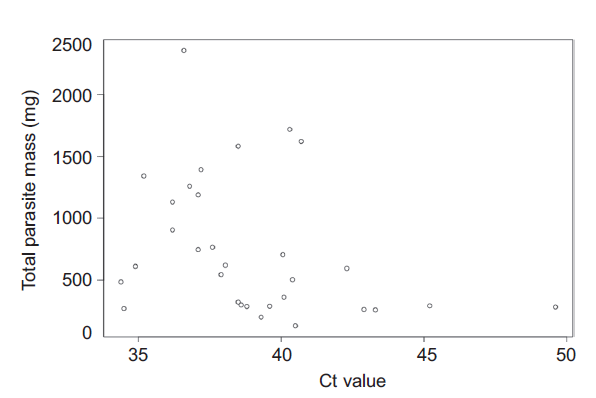
\includegraphics{Chapter2Images/parasitect.png} 
\caption{eDNA concentration co-varies with total parasite mass. ` Low cycle threshold (CT) values, which represent high levels of eDNA, are associated with a high parasite mass (Spearman correlation=-0.41, P=0.01, n=31) '.  The CT value plotted is the lowest value obtained from among the three replicates \citep{parasite}.}
\label{fig:parasite}
\end{figure}

Figure~\ref{fig:parasite} is a visualization of the CT scores obtained for the diseased fish. In general, parasite mass was negatively correlated with CT score. One fish was removed from the original 32 as it died before dissection could be performed. Hence there are 31 points plotted.






\section{Environmental Factors}


As interest in the study of eDNA grows, it is critical that researchers understand how environmental factors could influence detection protocols. The impact of environmental `covariates' such as weather, proximity to target organism or the time of day and how these impact eDNA concentrations and collection is still a subject of ongoing study \citep{cupwater}. In Chapter 5 we consider how these environmental covariates may impact eDNA concentrations in the field.
\vspace{5mm}



To further understand how environmental covariates may impact eDNA measurements, we consider the following case study. The Rocky Mountain tail frog \textit{Ascaphus montanus} and the Idaho giant salamander \textit{Dicamptodon aterrimus} are two species that are endemic to mountainous regions of Western North America \citep{amphibiandecline}. Both species are considered to be `secretive' and are especially difficult to study using standard sampling techniques. It is crucial that scientists and investigators understand how the results obtained via eDNA methodology may differ (or not) from standard techniques such as transect sampling or electrofishing.

\vspace{5mm}

In one study \citep{occupancyamphibians}, researchers collected eDNA samples from 13 streams in the South Fork Salmon River Sub-Basin, located in Idaho, USA, during the summer of 2011. In addition, multiple negative controls were taken more than 100km south of where either species is known to live.

\vspace{5mm}

In this study, researchers described four main goals. The first goal was to ``Develop and test alternative field protocols for sampling stream water for eDNA". The second goal was to ``Compare estimates of detection probability, density, biomass and occupancy obtained via different methods". The third goal was to examine how covariates (time of day, location in stream, etc) influenced eDNA detection and the fourth and final goal was to examine factors influencing precision of eDNA concentration estimates. 

\vspace{5mm}

Four of the original 13 streams were chosen to compare three distinct methods of sampling eDNA (In-Stream, Grab-and-filter and Grab-and-Hold). Researchers compared three field methods in four streams, direct filtration of stream water in the field (in-steam), water collected in a 1L Nalgene followed by immediate filtration (grab-and-filter) and water collected in a 1L Nalgene, stored over night and filtered in the lab the next day (grab-and-hold). Each of these three sampling methods has advantages and disadvantages with respect to time, money and effort (Goal 2).

\begin{figure}[H]
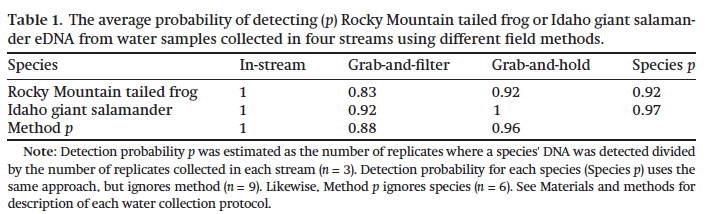
\includegraphics[scale=0.8]{Chapter2Images/rockymountain1.png}
\caption{Comparison of three eDNA sampling methods. Species p refers to the detection probability of the corresponding species \citep{occupancyamphibians}}
\label{fig:comparisonedna}
\end{figure}


Figure~\ref{fig:comparisonedna} illustrates a comparison of three eDNA sampling methods (Goal 2).  In stream methodology had perfect detection, but all three methods produced similar estimates. Note that `Method p' ignores species while `Species p' ignores method and averages over all methods. All three eDNA collection methods produced high detection rates. However, only `In-Stream' filtering led to perfect detection for both species. Researchers did not find any significant difference between any of the three collection methods. 
\vspace{5mm}


To research Goal 1, the researchers  set up standard sampling techniques (using thirty 1m transects randomly placed within 1km upstream of each of the 13 streams where they had taken eDNA samples).  Researchers then counted and weighed all larvae from either species on all the transects. The reason they chose larvae is because this is the most common life stage of the amphibians and thus can be used to infer information regarding adult populations. Larval density and biomass were calculated for each of the 30 transects and the average values were calculated.

\vspace{5mm}

Researchers then performed Backpack electrofishing on the four specified streams 500m upstream from where they had collected eDNA. Researchers then estimated giant salamander density by dividing the number of larvae caught by the total area they searched. Electrofishing allowed the researchers to assure that their methods of kick-net sampling were reliable. Kick-net sampling involves holding a net under the water and kicking the bottom of the substrate in an effort to direct organisms and materials towards and into the net. Indeed, results obtained via electrofishing were excellent predictors of how many larvae had been captured using kick-net sampling (which was done immediately prior to the start of the experiment in each of the four specified streams). (Simple linear regression on eDNA concentration obtained a $R^{2}$ of 0.96 and p-value of p=0.019).


\vspace{5mm}


To investigate the impact of covariates (Goal 3), researchers chose three of the thirteen streams for additional analysis. These were the Deadwood River stream, the East Fork Deadwood stream and the Weir Creek. In the Deadwood river and East Fork, eDNA concentration was measured using the in-stream method for tailed frogs in two reaches 50m apart over a 48-hour period. In Weir Creek, multiple eDNA samples were taken (every 50m for 2km). Following this collection, a three-day multiple removal process (electrofishing) of salamanders took place. The salamanders were removed, weighed and the exact location in which they were removed was recorded. This capture data was used to create a population distribution model for salamanders along the 2km Creek. This data was used to study whether eDNA concentration was impacted by the abundance of salamanders upstream of where the sample was taken.


\vspace{5mm}

For each of the thirteen streams, three replicate samples of surface water were collected. Each sample was taken by pumping 1L of water through a disposable filter funnel with a 47mm diameter cellulose nitrate filter paper. Negative controls were simply 1L of store-bought distilled water. Genetic analysis (qPCR) was then performed on the filter papers. DNA extracted from both species was used to create serial dilutions (standard curves) for comparison. In particular, samples of tissue taken from the tails of each species was used. To quantify the DNA concentration in the
original samples, researchers used a NanoDrop spectrophotometer to estimate the amount of DNA in each sample.

\vspace{5mm}

To compare eDNA concentration estimates obtained from the standard curve among the three different field methods (Goal 4), researchers used a mixed effect model with `stream' as the random effect. Analysis was performed using the SAS software \citep{SAS}. Mixed models are extensions of linear models that allow for the inclusion of both fixed and random effects. 

\vspace{5mm}

Researchers also compared stream-level occupancy and detection probability estimates obtained via standard sampling versus those obtained using eDNA methodology. To test whether eDNA concentration was correlated with abundance, researchers used a General Linear Model. Each of the thirteen streams was a sampling unit and the predictor variables were mean density, mean biomass or proportion of transects occupied (occupancy). The response variable was mean eDNA concentration and was calculated using the three replicate subsamples from each stream (obtained by referring to the standard curve).

\vspace{5mm}

To test for the effect of covariates, further analysis was carried out on the samples obtained from the three specified streams above (Deadwood, East Fork and Weir). Sample location was included as a predictor, along with time of day.

\vspace{5mm}

One main finding of this study was that eDNA detection probabilities does not appear to be influenced by water collection methods. 
In this study, eDNA methodology resulted in better detection rates then simple transect methods.
Finally, in this study, covariates such as time of collection did not appear to be of major impact on calculated eDNA concentration.
In Chapter 5, we consider the impact of environmental covariates on eDNA concentrations in the field.

\newpage

\subsection{eDNA movement}

Because eDNA of aquatic species is shed into streams or rivers, it is crucial that researchers understand how measurement of eDNA is impacted by movement in systems such as complicated, flowing water \citep{ednatransport}. In standing or still waters, measurement of eDNA has been widely used to estimate target species abundance \citep{biomass}. However, studies of eDNA within moving water systems are much less common. In order to study eDNA collected from moving water systems, it is important that researchers understand the biological and physical properties that influence retention and transport of eDNA travelling within these waters.  In Chapter 4, we fit a variety of non-linear models to account for flow and dilution. 

\vspace{5mm}


Researchers have suggested three major mechanisms that impact eDNA  moving systems. Firstly, there is \textit{Transport} (downstream movement driven by bulk water flow),
secondly there is \textit{retention} (deposition or capture by the streambed) and lastly, there is \textit{resuspension} (eDNA embedded in the streambed may become loose or free again) \citep{ednatransport}.

\vspace{5mm}

It has been demonstrated that eDNA in streams is significantly retained by the streambed as it moves down the stream and that concentration of eDNA decreases with downstream distance. Also, although eDNA is deposited on the streambeds, some of this eDNA will end up resuspended in the moving stream \citep{substrate}. More specifically, it has been shown that `fine' substrates such as sand retain more eDNA than `course' substrates such as pea gravel \citep{porous}.



\vspace{5mm}

 \citep{ednatransport}, asked three main questions corresponding to each of the three major mechanisms. 
1), ``How far does an average eDNA particle travel in streams with different hydrologic signatures and how might eDNA detection be used to infer where a species is located?"
2) ``Does surface-subsurface exchange trap eDNA in porous, benthic substrate interstices and does the presence of biofilms of organic matter play a role?"
3) ``Can resuspension from the streambed result in eDNA detection after the source of eDNA has been removed, and how does the characteristic of the streambed impact this?"

\vspace{5mm}


To study these mechanisms, researchers proposed three hypotheses. The first hypothesis was that  downstream transport of eDNA will be limited by hyporheic exchange rates (how quickly water is moving in and out of the stream). In Chapter 4 we  also consider the impact of flow on eDNA movement in a controlled experiment. Figure~\ref{fig:ednatransport} illustrates the three proposed governing mechanisms of eDNA movement in streams.



\begin{figure}[H]
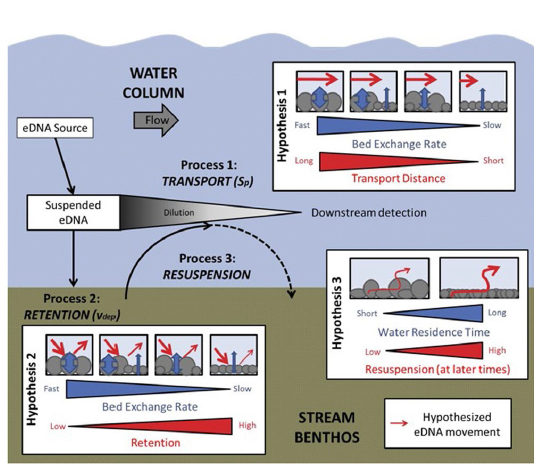
\includegraphics[scale=0.8]{Chapter2Images/ednatransport.png}
\caption{Conceptual diagram depicting the three governing processes of eDNA movement in streams: 1)
Transport, 2) Retention, and 3) Resuspension, and associated hypotheses for eDNA movement \citep{ednatransport}}
\label{fig:ednatransport}
\end{figure}

\vspace{3mm}

Researchers conducted experiments in four streams at the University of Notre Dame Linked Experimental Ecosystem Facility (ND-LEEF) in the summer of 2014. Each of the four streams are 0.4m wide, 7-10cm deep, and 60m long. The water is sourced from a head reservoir fed by groundwater. The four streams are nearly identical in all aspects except that each stream has differing benthic substrate lining the bottom.

\vspace{3mm}

Researchers collected water from a local pond that was known to have a high density of carp. This collected water was then pumped into the head of each of the four streams at a rate of 100mL/min. This was meant to simulate a carp at the head of the stream, whereby it was hypothesized the eDNA would flow or `transport' downstream. The injection of pond water was done for four hours. At the four-hour mark, 15 samples of 250mL were collected at predefined distances from the head of each stream. Once the pump was turned off (simulating fish removal), researchers continued to collect samples at regular timed intervals. The samples were stored and transferred to the lab, where qPCR was performed.

\vspace{3mm}

 To quantify the number of DNA copies in each extract, researchers created a synthetic standard curve and included it on each qPCR plate along with the DNA extracts. Since researchers knew the amount of DNA in their dilution series, they were able to create a standard curve for carp concentration. By comparing the known molecular weights with the obtained CT scores, the researchers were able to apply linear regression to create the standard curve. Moreover, the researchers were able to estimate the number of DNA copies in samples by dividing the estimated molecular weight of the DNA by Avogadro’s number. The LoD used in this study was 30 copies of DNA per reaction. The LoD was chosen based on the creation of the standard curve, as 30 copies of DNA per reaction resulted in a detection in 95\% of reactions.


\begin{figure}[H]
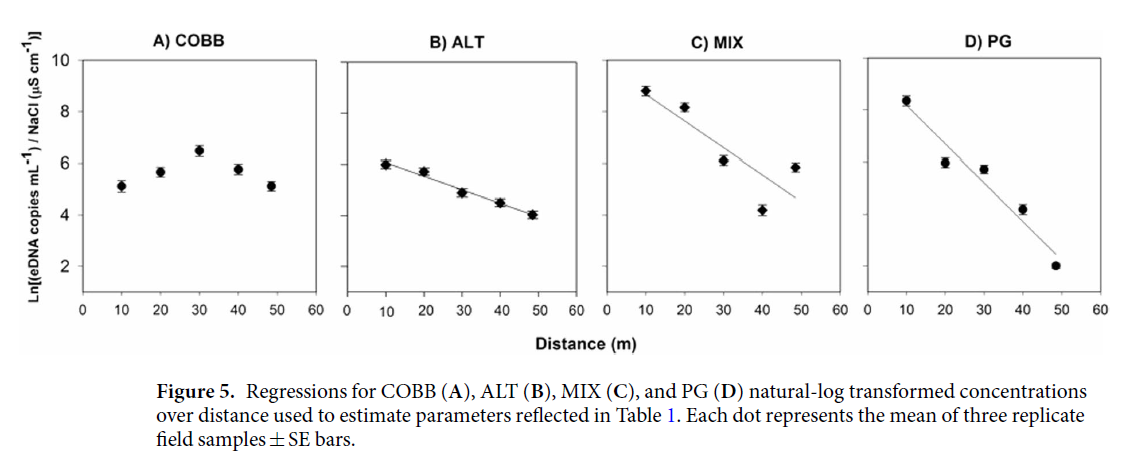
\includegraphics[scale=0.6]{Chapter2Images/transport2.png}
\caption{Results of the flow experiment \citep{ednatransport}. Stream PG has a smooth substrate, while COBB has course substrate. ALT and MIX have substrates in between course and smooth.}
\label{fig:ednatransport2}
\end{figure}

In general, eDNA concentration decreased as the distance from the head of the streams increased (Figure~\ref{fig:ednatransport2}). However, differences in substrate also resulted in different concentrations down the streams. COBB, ALT, MIX and PG are codes for each of the four streams. COBB has a more course substrate, while ALT and MIX have intermediate substrates. PG has a smooth substrate. NaCl was added to the mixture to help stabilize the DNA. The points plotted are the log transformed mean number of estimated copy numbers from each set of replicates, with the associated line of best fit created using simple linear regression.

\newpage



\subsection{Temperature}

Water temperature is known to be highly influential to the metabolism of fish \citep{tempmet}. The exact impact that temperature has on eDNA release is still not completely understood. It has been shown that in general, higher water temperature does increase the metabolism of fish (which may result in more DNA being shed).

\vspace{5mm}

 One study \citep{fishabundance} researched the question of how water temperature and the eDNA capture method impact the relationship between eDNA concentration and fish abundance. Researchers collected Brook Charr fingerlings from a fish hatchery in Cap-Sante, Quebec.  The fish were stored and returned alive to the lab. Fifteen tanks were prepared with water at $\ang{7}$ C, and another fifteen tanks were prepared with water $\ang{14}$ C.


\begin{figure}[H]
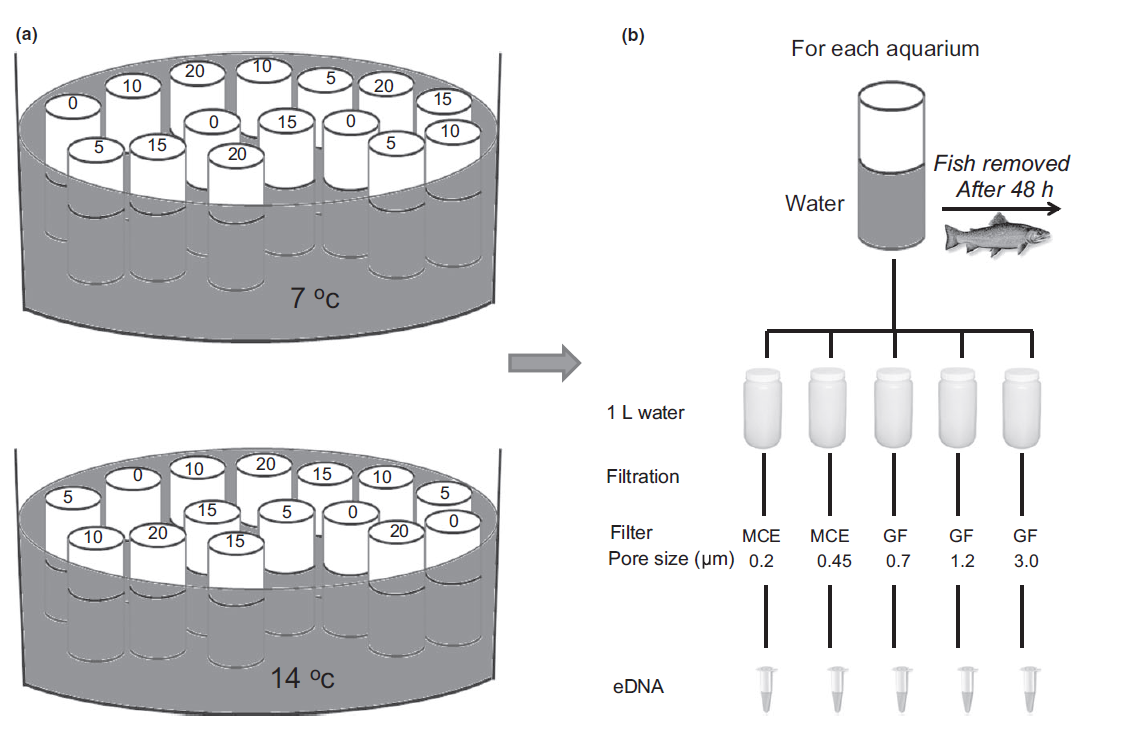
\includegraphics[scale=0.5]{Chapter2Images/brookchar.png}
\caption{Experimental design of Brook Charr exposed to $\ang{7 }$ C and $\ang{14}$C and (b) eDNA collection procedures  \citep{fishabundance}. Fish abundance for each
water temperature was randomly assigned. eDNA was captured via filtration (MCE, mixed cellulose ester filters; GF, glass fiber).}
\label{fig:brookchar}
\end{figure}

\newpage

For each of the two distinct temperatures, 0, 5, 10, 15 and 20, Brook Charr were placed into the 30 tanks (Figure~\ref{fig:brookchar}). For each temperature, each abundance of fish was repeated three times. That is, three tanks at $\ang{7}$ C contained 5 fish and three tanks at $\ang{14}$ C also contained 5 fish. The same was done for each number of fish. The zero fish triplicates represent negative controls, i.e. an abundance of 0.

\vspace{5mm}

The total biomass of fish in each tank was measured by comparing the weight of the tanks prior to the addition of the fish to the weight after they were added. The fish were then given five days to live in each tank. Each tank was then removed and let to sit in the dark for 48 hours, at which point the fish were removed. Once removed, the water in each 1L triplicate was mixed and then filtered using various filters and pore sizes to collect eDNA. DNA was extracted using the salt extraction method. A 139-basepair unique to Brook Charr was used as the target DNA. A standard curve was created using known 7 known dilutions of Brook Charr eDNA. eDNA concentration of samples was then quantified using real-time Taq-Man PCR and comparison to the 7-point standard curve previously created.


\vspace{5mm}

A Mann-Whitney test was used to test for significance in the mean eDNA concentration between the two separate temperatures (there were 150 fish for both temperatures for a total of 300 fish).
A Cook’s distance test was used to detect potential outliers and influential points. At all levels of fish abundance, higher eDNA levels (more concentrated) were found in the $\ang{14}$ C samples compared to the $\ang{7}$ C samples when using glass fiber (GF) filters. For a few filters that are known to have a low level of eDNA collection, such as MCE(2 $\mu L$), differences in eDNA at the two temperatures were not detected.

\vspace{5mm}
The results of this experiment showed that the concentration of eDNA  did increase significantly at higher temperatures. Researchers hypothesized this may be due to the fact that fish mobility is increased at higher temperatures \citep{fishmobility}, moreover at higher temperature the rate at which skin cells are shed and other secretions are released is increased.  Hence, temperature may need to be considered when a data analysis on eDNA on aquatic species is performed. This is particularly important when using fine filters that are known to capture high levels of eDNA. In Chapter 5, we consider the possible impact of temperature on eDNA concentrations as well. 
\startchapter{Density Experiment}
\label{chapter:newsol}

\subsection{Introduction}

 The \textit{Density Experiment} was conducted in the summer of 2015 \citep{fishforensics,hatchery}. The goal was to investigate the relationship between Transformed CT values (`TCT') and Coho Salmon `density’ (or the similar measurement of biomass). CT is the `Cycle Threshold' and we define TCT=50-CT.  The experiment consisted of manipulating juvenile Coho salmon densities in treatments of 1, 2, 4, 8, 16, 32, and 65 fish in replicated 10,000L tanks.


\begin{figure}[H]
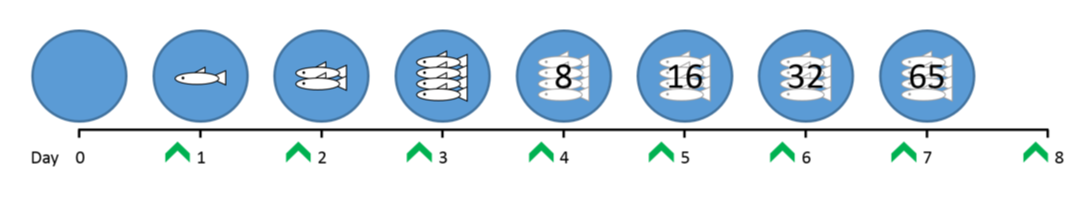
\includegraphics[scale=0.6]{Chapter3Images/samplingscheduleday.png}
\caption{ Sampling schedule for the Density Experiment \citep{berg}.}
\label{fig:densityschedule1}
\end{figure}

Figure~\ref{fig:densityschedule1}  \citep{fishforensics} provides an overview of the experimental schedule. For each main tank, Coho were added throughout the week of the experiment (indicated by the green arrows). On day one, one fish was added to the tank. On each of the following days of the week, fish were added until on day 7 there were 65 fish.

\vspace{3mm}

There were four 10,000L Tanks, numbered 19, 20, 21 and 24 for the main density experiment. From each tank, sample replicates of water were taken, usually five per tank.
For each fish, the biomass in grams was also recorded. The average mass of each fish used in the experiment was 5.69 grams. As the amount of water in each tank in this experiment was fixed, we expect that as biomass increases, the CT score should decrease (as we would expect more eDNA);  hence, the TCT should increase.

\begin{figure}[H]
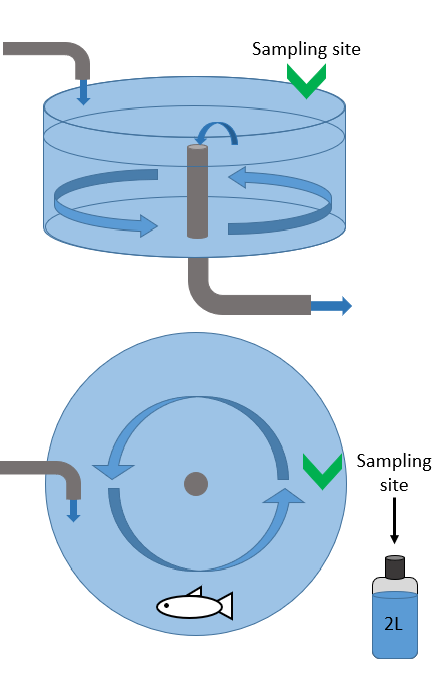
\includegraphics{Chapter3Images/goldstreamupdate.png}
\caption{The general sampling methodology for the density experiment \citep{berg}.}
\label{fig:samplingdensity}
\end{figure}

\newpage

Figure~\ref{fig:samplingdensity} illustrates the method in which samples were taken from the tanks. To sample from the tanks, 2L bottles were filled with water by submersion approximately 0.5m from the edge of the tank. The water was then filtered through 47mm diameter 0.45$\mu$m mixed-cellulose ester (MCE) filter membranes. From each sample replicate, eight technical replicates were obtained. These technical replicate samples were then evaluated using qPCR for the presence of Coho eDNA. Each unique set of eight technical replicates were assigned a unique ``sort.code". That is, every member that came from the same group of eight technical replicates had the same sort code. Note that one set of technical replicates, corresponding to sort.code=128 was discarded before analysis due to lack of integrity in the lab (Sample.replicate 3 of Tank 20, 65 Fish). 

\vspace{5mm}

In order to detect Coho salmon specifically, a DNA assay,  eONKI4 was used in combination with qPCR. To ensure quality of the eDNA, samples first underwent integritE-DNA tests. These tests combine a probe and a primer to amplify chloroplast DNA that appear pervasively in freshwater systems. Samples that failed the integritE-DNA test were cleaned using the Zymo OneStepTM PCR Inhibitor Removal Kit  and tested again. If the sample failed a second time, it underwent an inhibitor removal. If the sample still failed to pass the integritE-DNA test after inhibitor removal, it was excluded from the data to minimize the presence of false negatives. The qPCR analysis using the eONKI4 assay was conducted in the lab of Dr. Caren Helbing at the University of Victoria. Figure~\ref{fig:densityschedule} is a visualization of the process of DNA integrity validation. integritE-DNA tests were performed on samples prior to using qPCR to search for Coho eDNA. Before the experiment began, the tanks were bleached to clean any residual eDNA or materials that may have been present in the tanks. integritE-DNA test combines a probe and a primer to amplify chloroplast DNA that is pervasive in freshwater systems. 

\vspace{5mm}


For 1, 2, 4, 8, 16, and 32 fish, 6*4*5*8=960 observations were recorded. For each set of these six numbers of Coho, there were four tanks, for each tank there were five sample replicates, and for each sample replicate there were eight technical replicates.
For 65 Fish, there were 3*5*8+4*8=152 observations. For 65 fish there were three tanks with five sample replicates and one tank with four, for each sample replicate there were eight technical replicates.

\vspace{5mm}

A small pilot experiment was also conducted during the summer. The pilot experiment used smaller tanks, tanks 1, 2, 3 and 4.  Samples were taken from smaller tanks that only contained hatchery water and no Coho. The pilot experiment was used to gain insight regarding possible background signals in the hatchery waters.



\begin{figure}[H]
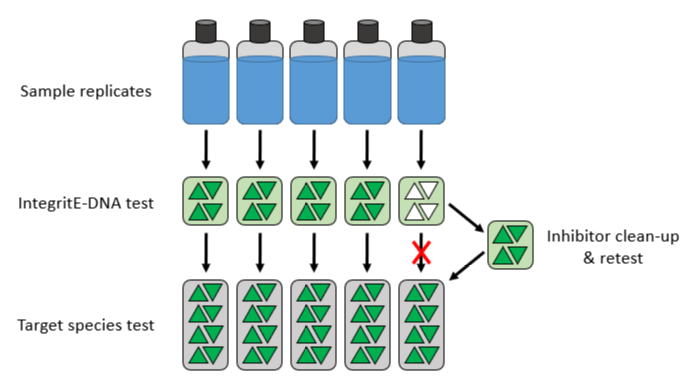
\includegraphics[scale=0.75]{Chapter3Images/integritE.png}
\caption{ Basic procedure for analyzing eDNA. Sample replicates were first certified using an integritE-DNA test before testing for Coho eDNA \citep{berg}.}
\label{fig:densityschedule}
\end{figure}


\section{Summary Statistics}

We now provide several tables that summarize features of the experiment. For example, we include tables listing the numbers of fish and which tanks they belonged to. Tables were created in R using the `kableExtra' package \citep{kable}.

\begin{table}[H]
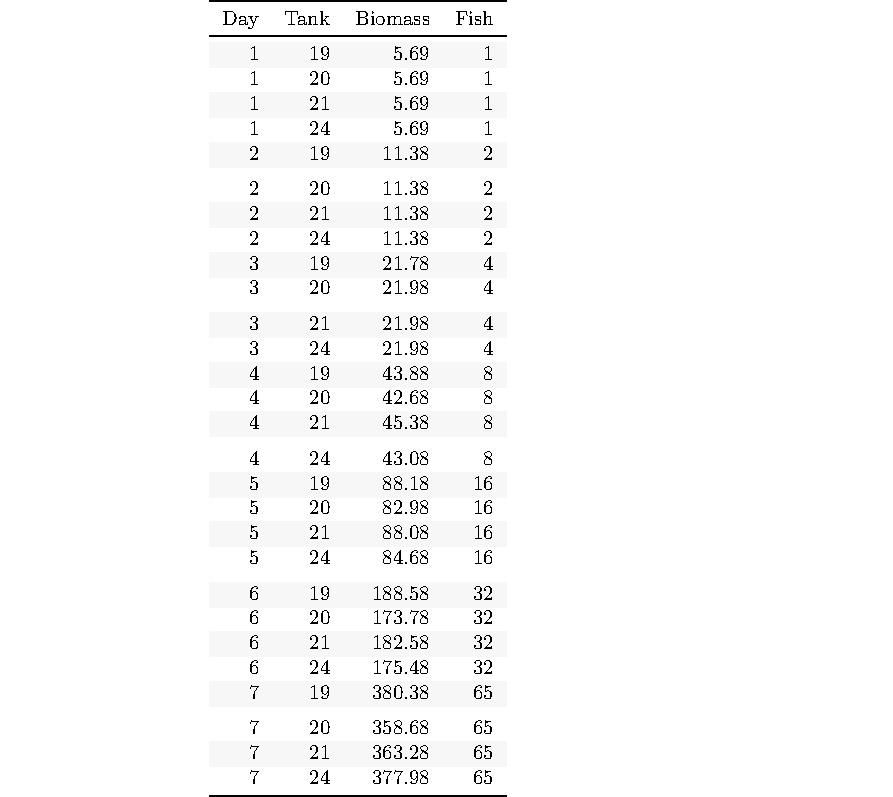
\includegraphics{Chapter3Images/kable1test.pdf}
\caption{\hspace{1mm}Table summarizing biomass (g) per tank and day.}
\label{lab:kable1}
\end{table}

Table~\ref{lab:kable1} provides the weight and number of the fish in each tank. For every day for a week, the amount of fish in the tanks (and hence the biomass) was doubled (except on the seventh day, it was doubled plus one to make 65 fish)


\begin{table}[H]
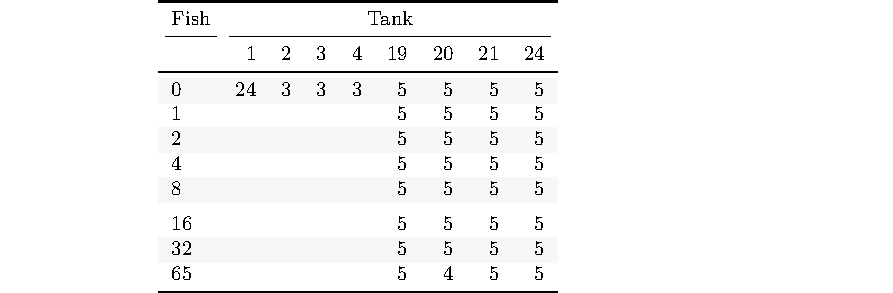
\includegraphics{Chapter3Images/kable2fixed2.pdf}
\caption{ \hspace{1mm}Summary of the number of sample replicates for each corresponding number of fish and tank number.
}
\label{lab:kabel2}
\end{table}

Table~\ref{lab:kabel2} provides the number of sample replicates that were taken from each tank, and how many fish were present in that tank. Tanks 1, 2, 3, 4, 19, 20, 21 and 24 all had samples taken in which there were zero fish. However, for most levels of fish density, such as 16 fish or 32 fish, only tanks 19, 20, 21 and 24 were used. In general, five sample replicates were taken from each of the four main tanks for each level of fish density (except for tank 20, 65 fish).

\begin{table}[H]
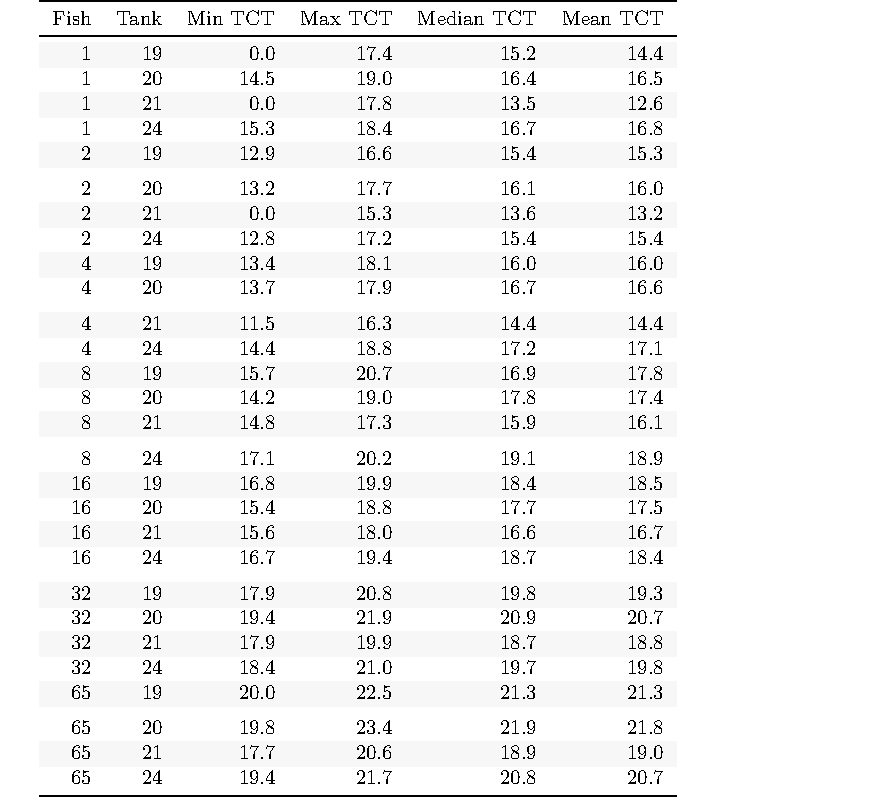
\includegraphics{Chapter3Images/kable3fixed2.pdf}
\caption{\hspace{1mm} Summary of the minimum, maximum and median TCT for each number of fish and tank.}
\label{lab:kabel3}
\end{table}

Table~\ref{lab:kabel3} provides several summary statistics for TCT values obtained. For each number of fish and tank, there were five sample replicates, and for each sample replicate there were eight technical replicates. Hence the maximum, minimum and median calculations use 5 x 8= 40 measurements each. Because one set of technical replicates was discarded from 65 fish, tank 20, only 32 measurements were used for that set of summary statistics.


\begin{table}[H]
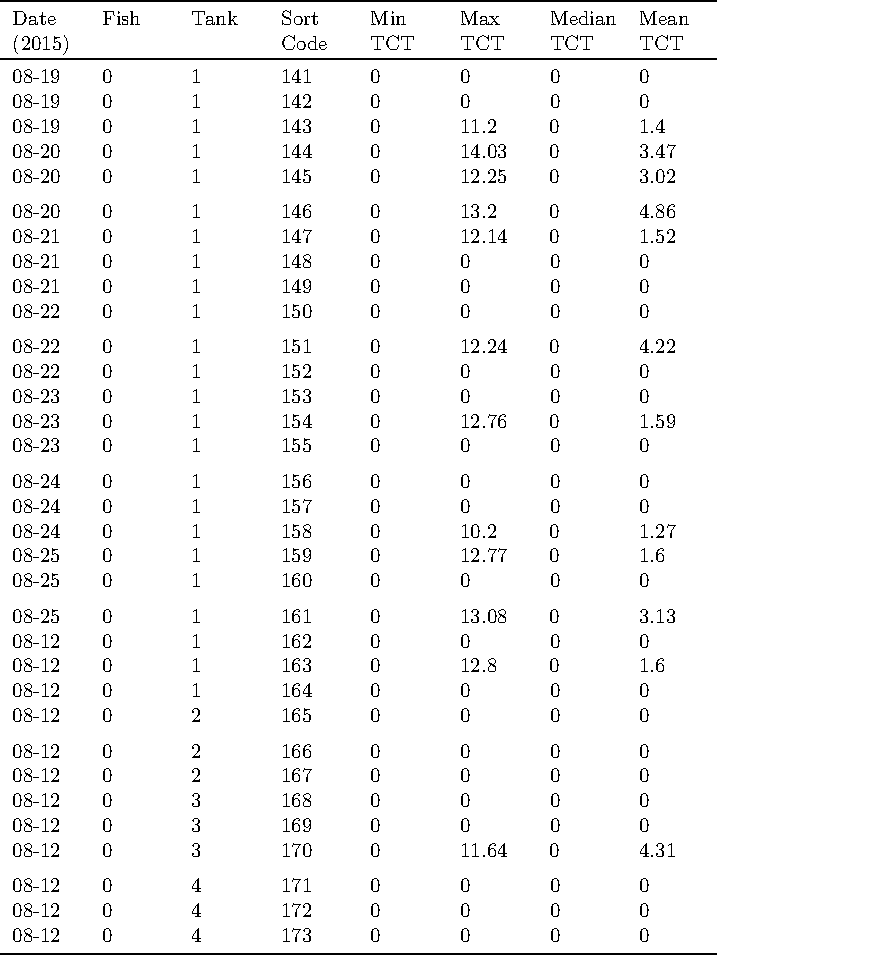
\includegraphics{Chapter3Images/kable4new.pdf}
\caption{  \hspace{1mm}These samples correspond to the Pilot experiment. They were taken to give an insight on the TCT background signal at the hatchery. We include the date for which the sample was taken, the tank, the sort code, and the summary statistics.}
\label{lab:kabel4}
\end{table}

Table~\ref{lab:kabel4} summarizes the samples that were taken concurrently over the course of the seven days in which the density experiment took place. The sampling began on August 19, 2015 and continued until August 25, 2015. These samples correspond mostly to a smaller tank (tank 1) and were taken during the pilot experiments. Samples corresponding to sort codes 162-173 are also part of the pilot experiment but were taken earlier on a single day (August 12). 


Finally, we include a table that summarizes the negative controls for the four main tanks.

\begin{table}[H]
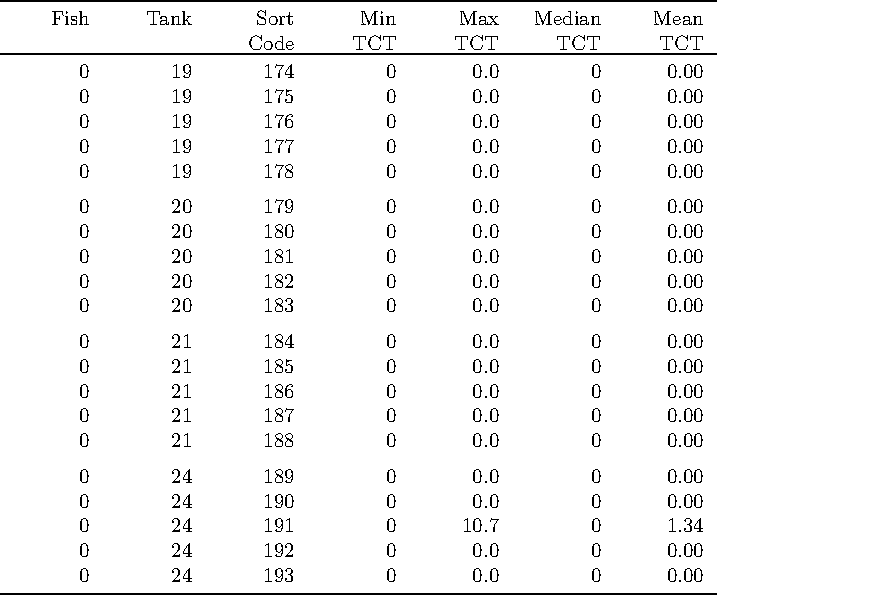
\includegraphics{Chapter3Images/kable5fixed2.pdf}
\caption{ \hspace{1mm}Pre-fish, negative controls, taken over all of the tanks. The calculations are taken over the eight technical replicates. Notice we had a single TCT of 10.73 in tank 24, indicating an outlier. }
\label{lab:kabel5}
\end{table}



Table~\ref{lab:kabel5} summarizes the pre-fish negative controls. Samples were taken prior to the start of the experiment from the four main experiment tanks (tanks 19, 20, 21 and 24).
\section{Density Plots}

 
Figure~\ref{lab:introplots122} shows the relationships between TCT and number of fish in each tank. Recall that for each sample replicate, there are eight technical replicates.


\begin{figure}[H]
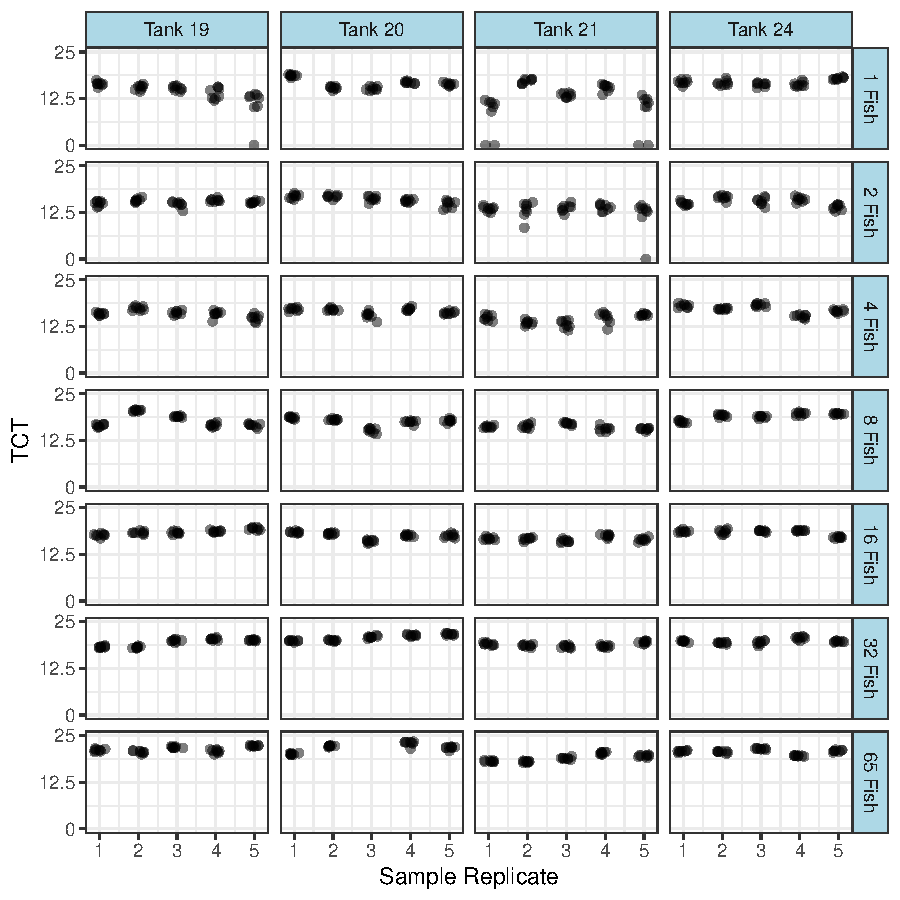
\includegraphics{Chapter3Images/gt.pdf}
\begin{center}
\caption{\hspace{1mm} Exploratory plots that plot the TCT for each number of fish in each tank. Each sample replicate has 8 technical replicates, each technical replicate has a TCT. }
\label{lab:introplots122}
\end{center}
\end{figure}








 In general, we notice TCT tends to increase as the number of fish increases. Although we have a relatively consistent increase in TCT as number of fish increases, there are several outliers. In particular, there are outliers for 1 Fish, Tank 19 and for 1 Fish, Tank 21. This may indicate that the presence of eDNA may not always be picked up in the lab. Although the sample had several technical replicates which did contain eDNA, some from the same sample replicate did not. As the density of fish increased, we see that we no longer have any major outliers, and the test for eDNA did not fail to pick up the presence of Coho eDNA.
  

\vspace{5mm}


Figure~\ref{lab:introplots1232} shows TCT values for the sample replicates taken for zero fish.  These are negative controls corresponding to sort codes 162-193 in Table 3.5. They were taken over a variety of tanks and days. The plots for tanks 1, 2, 3 and 4 correspond to the pilot experiment and give an idea of hatchery signal. The plots for tanks 19, 20, 21 and 24  are from `true' pre-fish negative controls for the density experiment.



\begin{figure}[H]
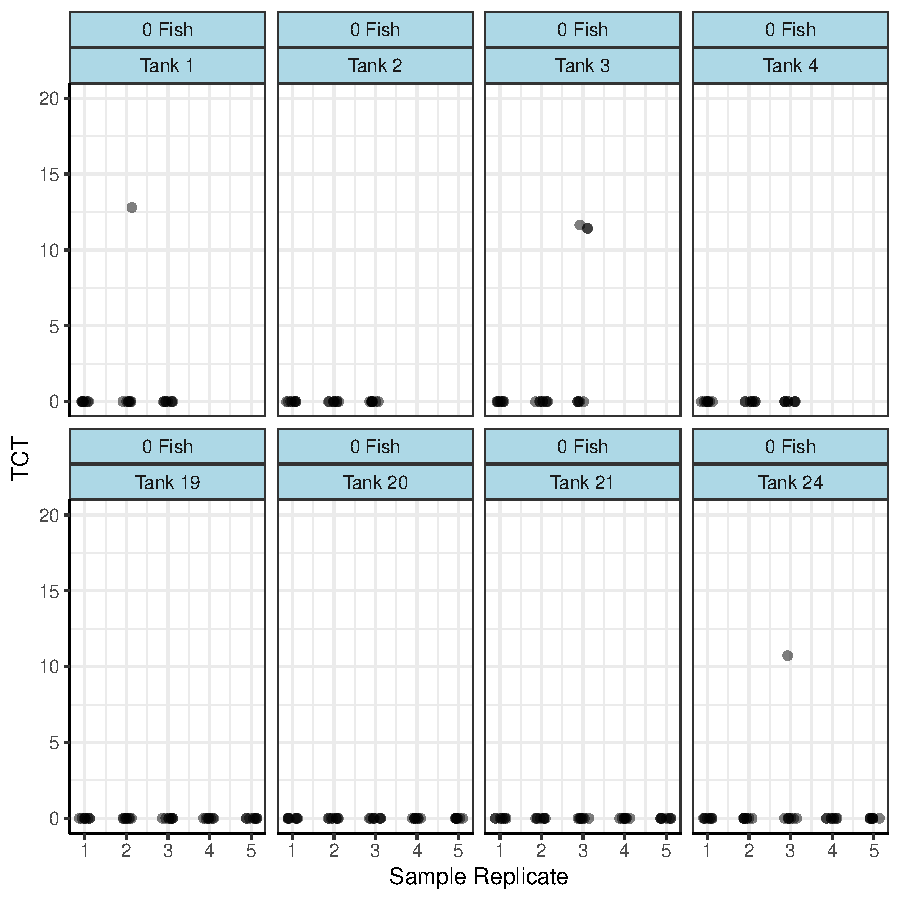
\includegraphics{Chapter3Images/gz2.pdf}
\begin{center}
\caption{\hspace{1mm} Plots of TCT for zero fish (Negative Controls). Notice there exists a slight Coho eDNA signal. This means that there could be Coho DNA present in the hatchery water. }
\label{lab:introplots1232}
\end{center}
\end{figure}




\begin{figure}[H]
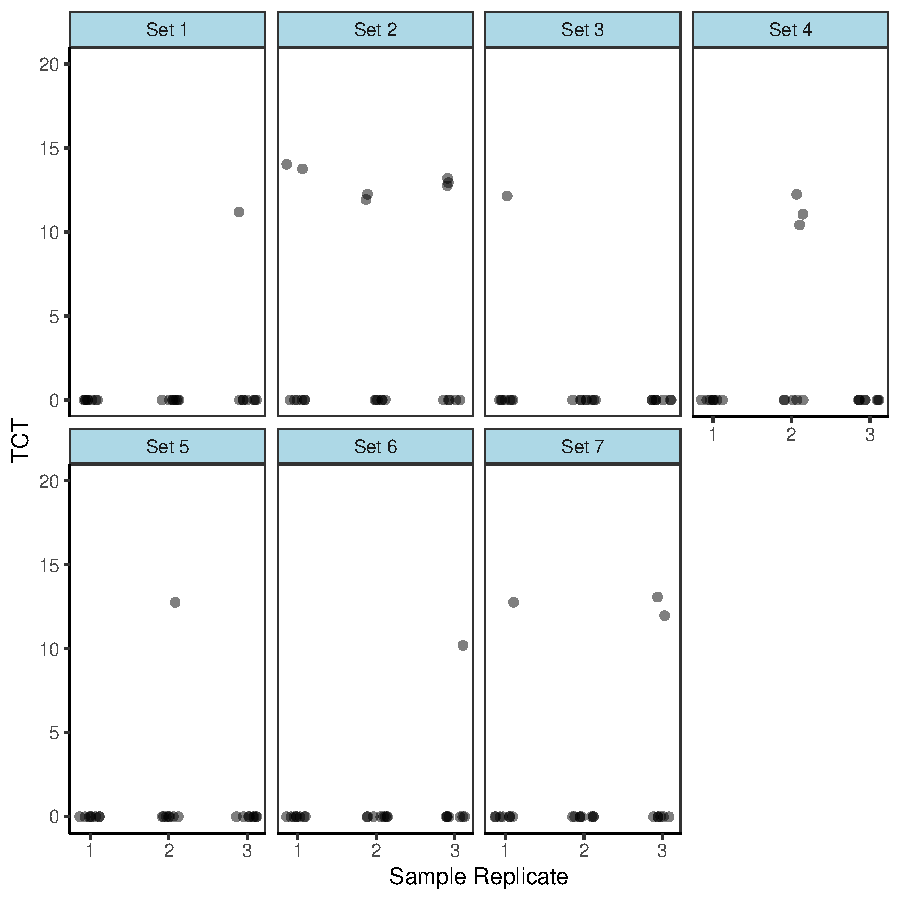
\includegraphics{Chapter3Images/gz3.pdf}
\begin{center}
\caption{\hspace{1mm}Additional plots of TCT for zero fish taken from tank 1. }
\label{lab:introplots123222}
\end{center}
\end{figure}





Figure~\ref{lab:introplots1232} and Figure~\ref{lab:introplots123222} are both plots of TCT values obtained from tanks in which no fish were present. Figure~\ref{lab:introplots1232} contains the negative controls for the main experiment, as well as TCT values obtained from the pilot experiment. Figure~\ref{lab:introplots123222} contains additional plots of TCT measurements taken from the pilot experiment. In general, the hatchery water appears to contain a small background signal of Coho. 
\section{Models for Density (Median)}

We fit a variety of competing linear models using the `lm' function in R \citep{Rprogram}. We used the median transformed CT of the technical replicates as our response variable. Initially, we fit a simple linear model, l.one.line, where we fit a least squares line of best fit for our response variable by considering only a single input predictor, log2(Biomass). To plot models, we used the base R plot function and the ggplot2 package \citep{ggplot}, as well as the `ggthemes' package \citep{ggthemes} and the `latex2exp' package\citep{latextoexp}. Next, we fit two multiple linear models. The first model named lmparallel.tfac is a multiple linear model with the two predictors, Log2(Biomass) and tank. We also fit a model called lfull.tfac, which incorporates both Log2(Biomass) and tank and also the interaction between Log2(Biomass) and tank.


\begin{figure}[H]
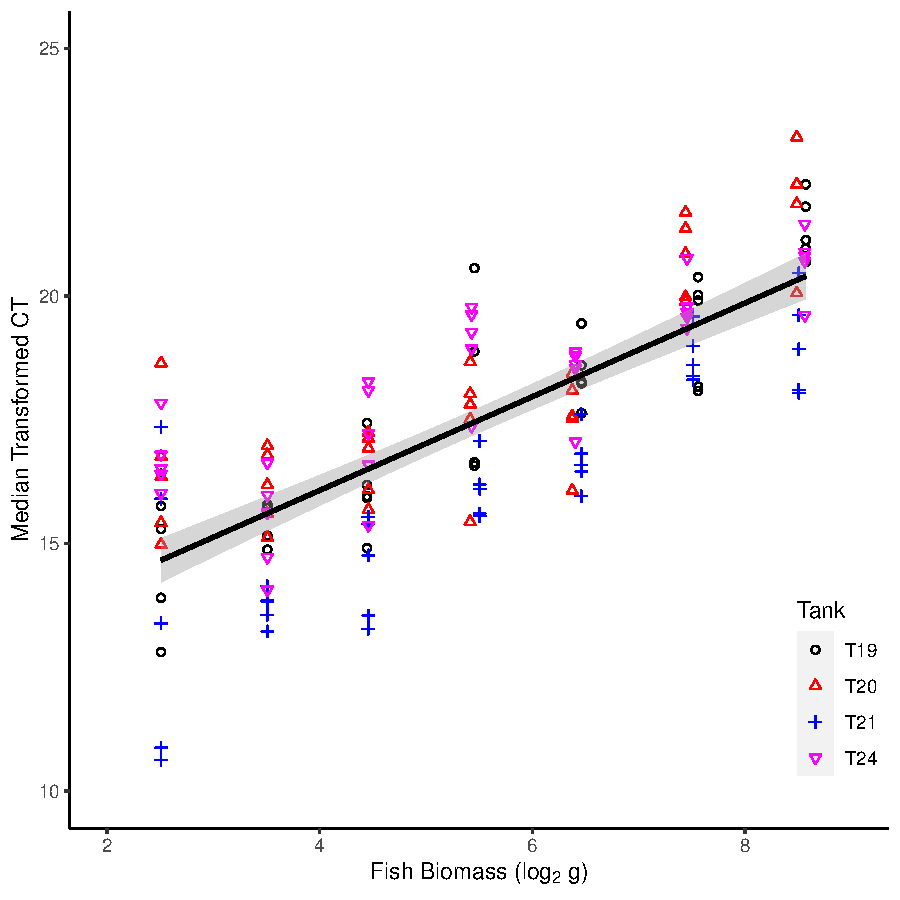
\includegraphics{Chapter3Images/ggplotnew.pdf}
\caption{ Median Transformed CT versus Log2(Biomass). The fitted regression line, l.one.line and the 95 \% confidence intervals are included. Each of the four tanks has an associated color and shape.}
\label{fig:medct1}
\end{figure}

%\begin{table}[H]
 %\begin{singlespace*}
%\verbatiminput{tablesandimages/loneline.txt}
%\caption{Summary of our first simple model,  l.one.line. This model only includes an intercept and a biomass term.}
%\label{lab:loneline}
%\end{singlespace*}
%\end{table}


\begin{table}[H]
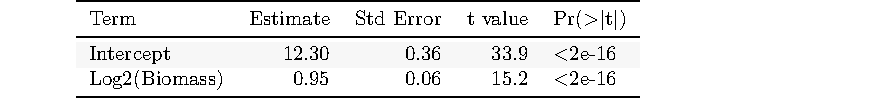
\includegraphics{Chapter3Images/lonelinekable.pdf}
\caption{Summary of our first simple linear model,  l.one.line. This model only includes an intercept and a biomass term. The $R^{2}$ value is 0.626.}
\label{lab:loneline}
\end{table}


Table~\ref{lab:loneline} is a summary of a simple linear model (l.one.line)  fit using the lm function. The estimated intercept of the model is 12.30 with a standard error of 0.36. The model also produces an estimate for the slope of 0.95 with a standard error of 0.06.  The p-value for both estimates is very small. The p-values are in the $Pr(>|t|)$ column. The p-value refers to the probability that we observe what we did, given that the null hypothesis is true. The null hypothesis in this case is that the associated parameter is zero. Since the p-value is so small, we can reject the null hypothesis (at a significance level of 0.05) and conclude that those terms are significantly different from zero. 

\vspace{12pt}


Figure~\ref{fig:medct1} confirms visually that as fish biomass increases, Log2(Biomass) in particular, median TCT also increases. This makes sense, as with more fish we would expect more residual eDNA, and thus a lower CT score (and hence a higher TCT score). The $R^{2}$ is $0.626$ which means that this simple model already does a relatively good job at explaining variation in the data.

\newpage

We also plot regression lines obtained by considering each tank on its own and allowing the intercept to vary. 


\begin{figure}[H]
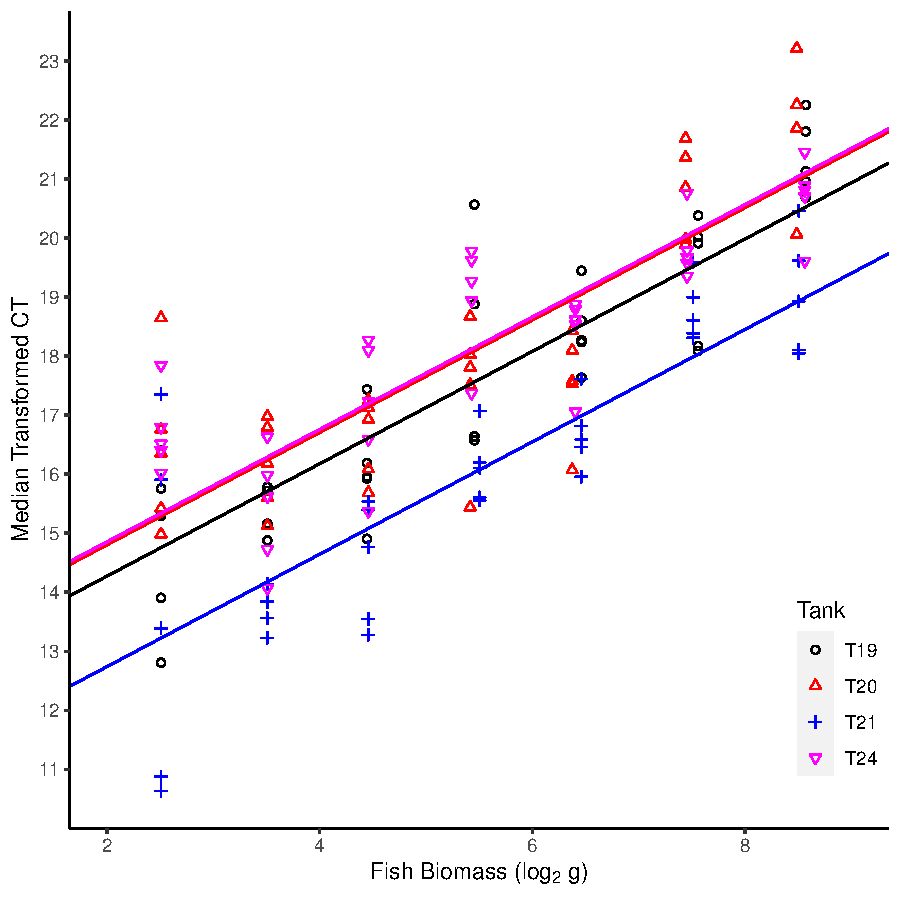
\includegraphics{tablesandimages/parfits.pdf}
\caption{ Lines of best fit for Median Transformed CT versus Log2(Biomass) for each specific tank. This is equivelent to the model  lmparallel.tfac.}
\label{fig:medpar}
\end{figure}

Figure~\ref{fig:medpar} is the plot of the model  lmparallel.tfac. In this model, only the intercept is allowed to vary for each tank, but the slope remains the same. We see again tank 21 has a siginficantly lower intercept than the other tanks.


\vspace{5mm}

% \begin{table}[H]
 %\begin{singlespace*}
%\verbatiminput{tablesandimages/lmparallel.txt}
%\caption{This model, lm.tfac considers each tank as a predictor.}
%\label{lab:lmparallel}
%\end{singlespace*}
%\end{table}

 \begin{table}[H]
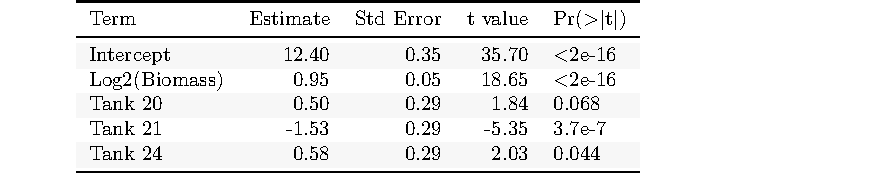
\includegraphics{Chapter3Images/lmparallelkable.pdf}
\caption{Parameter estimates and standard errors for model  lmparallel.tfac where Log2(Biomass) and tank are predictors. The $R^{2}$ value is 0.756.}
\label{lab:lmparallel}
\end{table}



Table~\ref{lab:lmparallel} provides a summary for the model  lmparallel.tfac. This model has a common slope parameter for Log2(Biomass), but allows the intercept to change for each tank.  The intercept changes depending on which tank the point belongs to according to the estimates in Table~\ref{lab:lmparallel}.The baseline for tank comparisons is tank 19. Compared to tank 19, tank 20 and tank 24 appear to result in slightly higher median TCT values. This can be seen by the coefficients that are greater than 0, which means for those tanks we have in increase in median TCT compared to our baseline tank. For tank 24, the p-value is $0.044$, which indicates significance. However, we see a clear effect in Tank 21, which results in a lower median TCT compared to the other tanks, with a very small p-value of 3.7e-07 indicating strong evidence at the 0.05 alpha level. One possible explanation for this is that tank 21 obtained a more complete bleaching than the other tanks, hence resulting in less eDNA when sampled. This would cause a higher CT and hence a lower TCT.  The adjusted $R^{2}$ for this model is $0.746$, which is much larger than the adjusted $R^{2}$ of l.one.line (0.623). This means that our model does a good job at explaining the variation in the data. The adjusted $R^{2}$ contains a penalty term for the number of predictors in the model. 





\newpage

Finally, we also consider a model that includes the possible interactions between tank number and biomass.  This model allows for a different slope and intercept for each tank and also allows for interactions between tank and biomass. This is the model plotted in Figure~\ref{fig:lmedspecific}, and we will see that results obtained from this model are equivelent to considering each tank in isolation.

\begin{figure}[H]
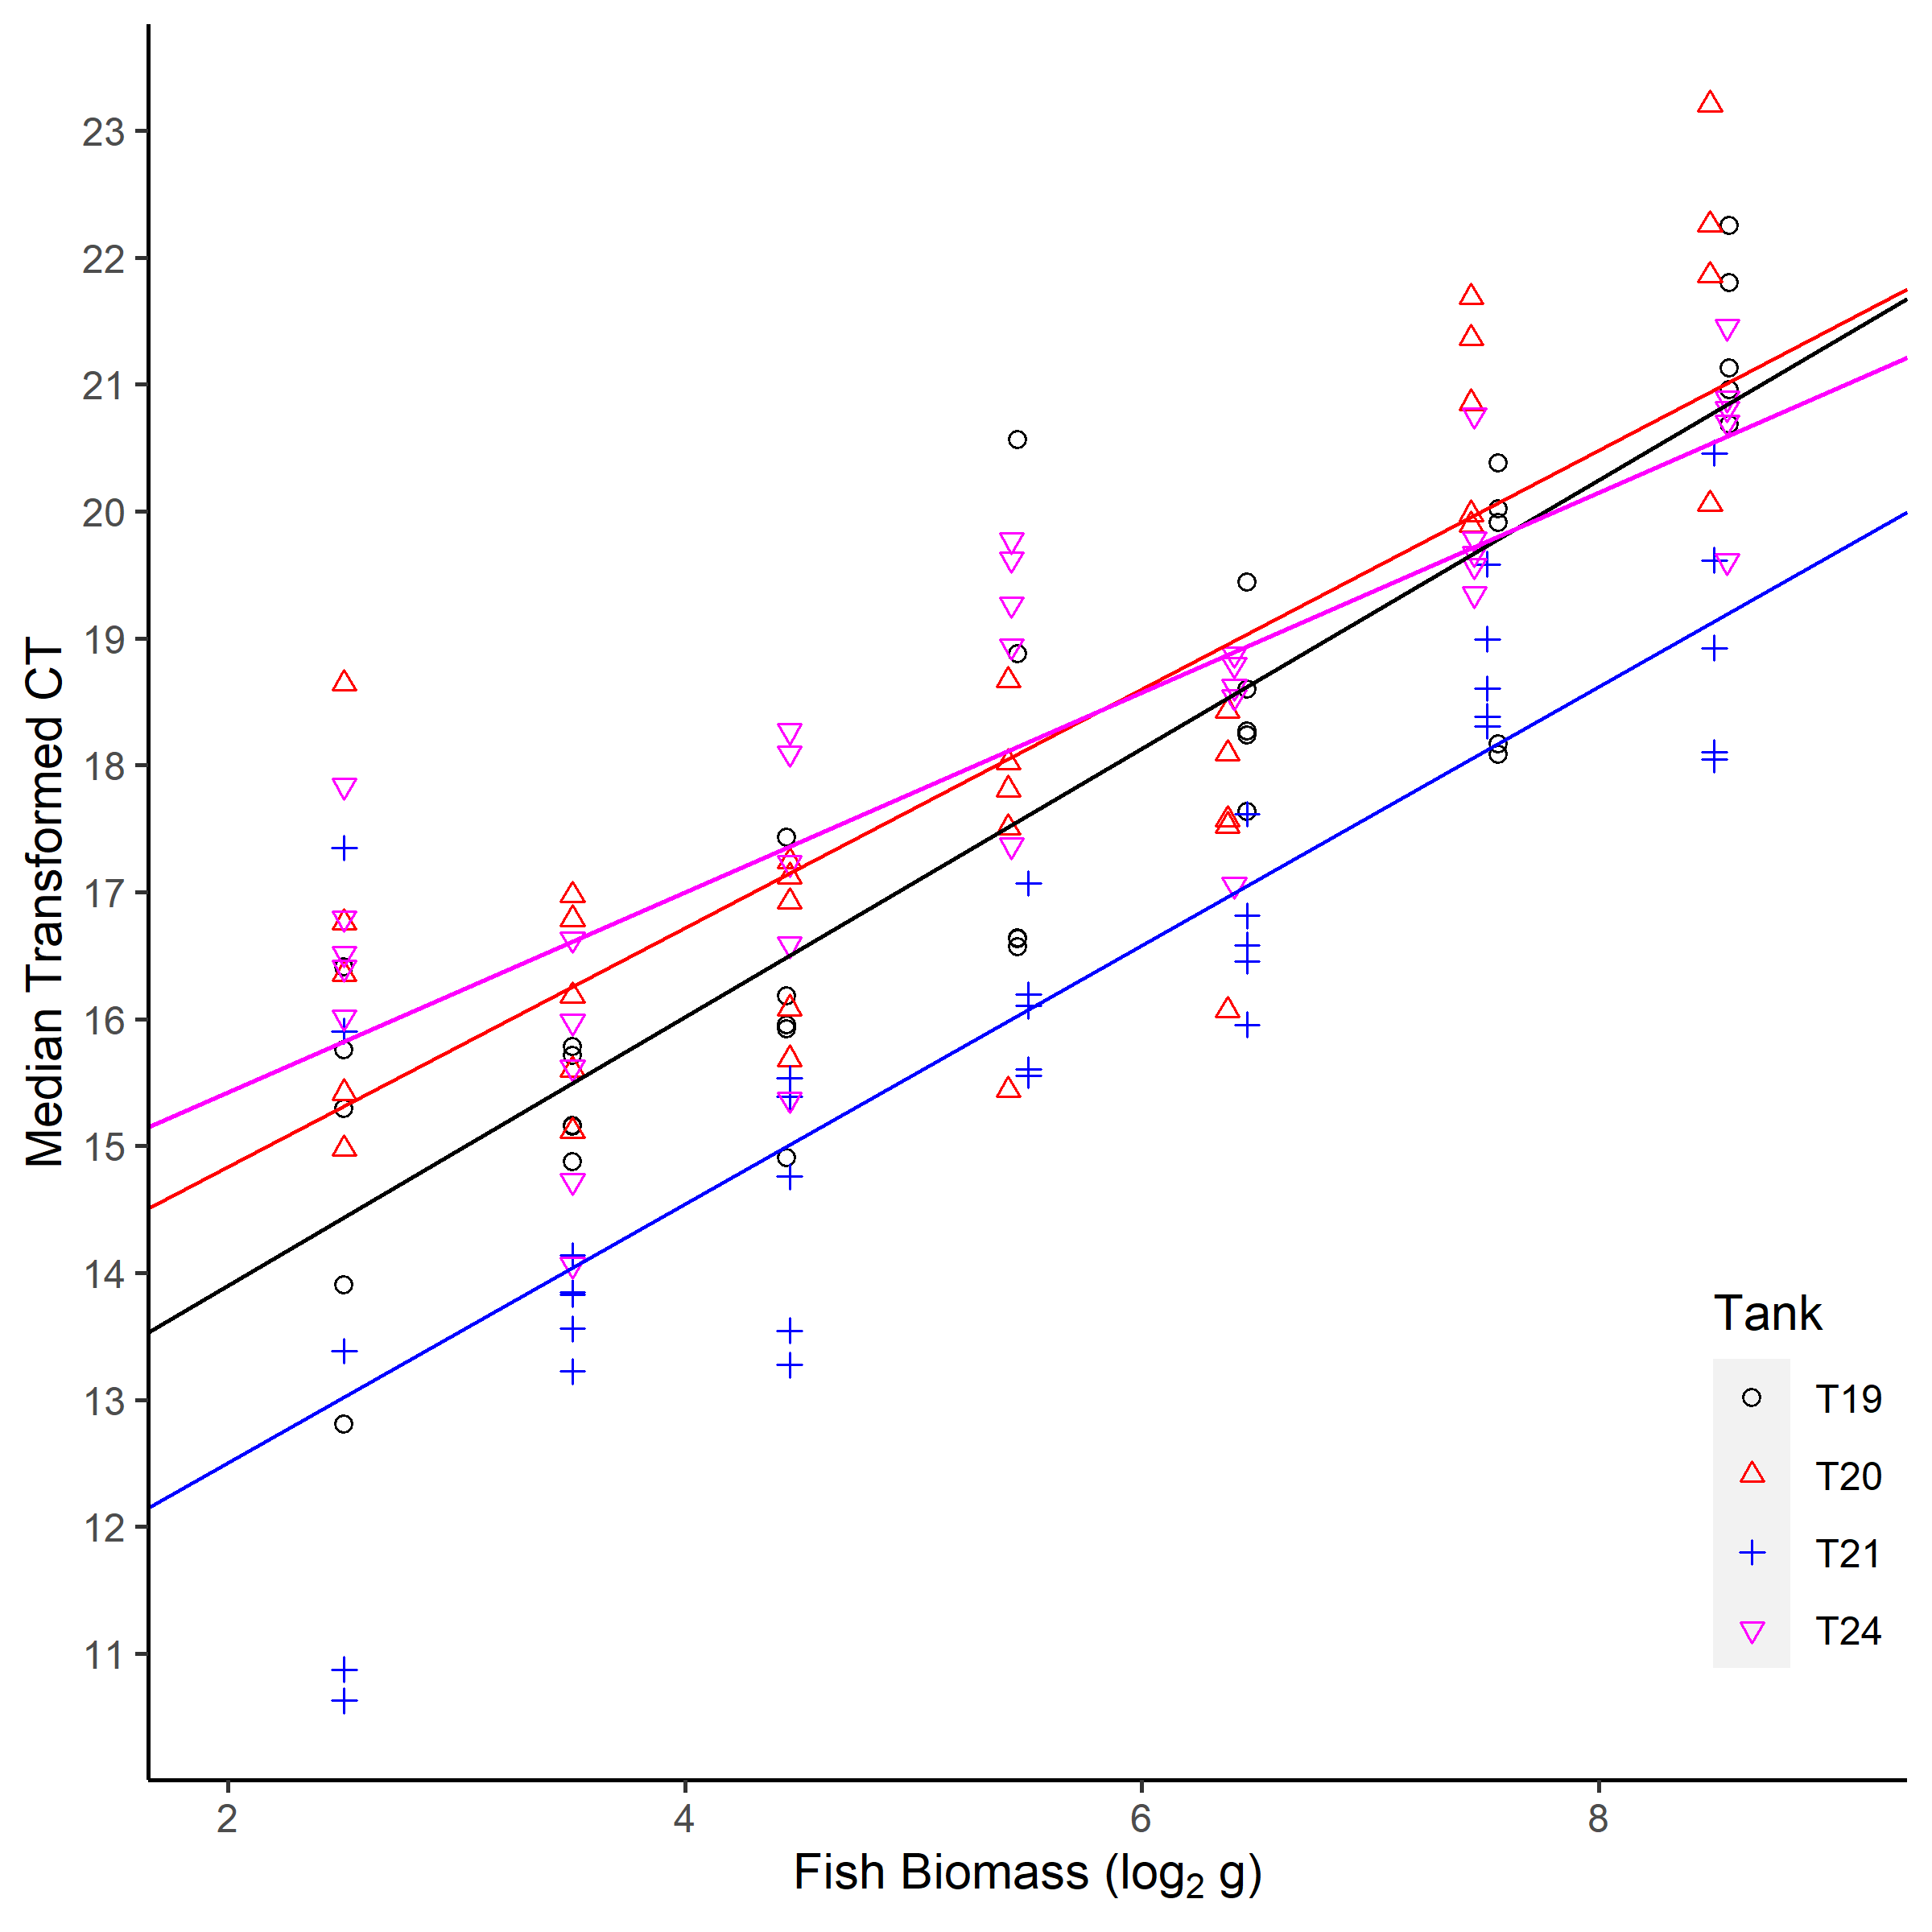
\includegraphics{Chapter3Images/ggplotnew2.png}
\caption{ Lines of best fit for Median Transformed CT versus Log2(Biomass) for each specific tank. This is equivelent to the model lfull.tfac.}
\label{fig:medct33}
\end{figure}

Figure~\ref{fig:medct33} is a plot of regression lines obtained by applying regression over each individual tank. In this regression, each tank has its own intercept and own slope. Figure~\ref{fig:medct33} seems to indicate that tank likely impacts the result of median TCT. Thus we fit a model that included tank as a predictor. 



\begin{table}[H]
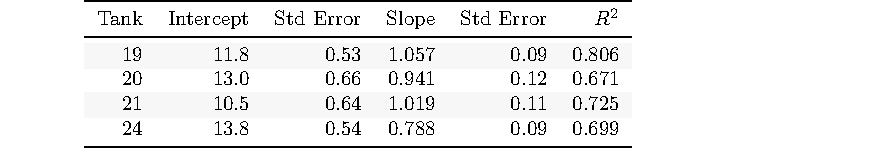
\includegraphics{tablesandimages/sumtable1.pdf}
\caption{Table summarizing simple linear regression on Log2(Biomass) when each tank is considered in isolation for median TCT.}
\label{fig:lmedspecific}
\end{table}



Table~\ref{fig:lmedspecific} summarizes the results of applying simple linear regression to each tank in isolation, obtaining separate estimates for each intercept and slope. Tank 21 has the smallest intercept, while tank 24 has the largest intercept. The slopes are similar, however tank 24 has a noticeably smaller slope. The $R^{2}$ are all quite high, but tank 19 alone has the highest $R^{2}$. 



   \vspace{12pt}



\begin{table}[H]
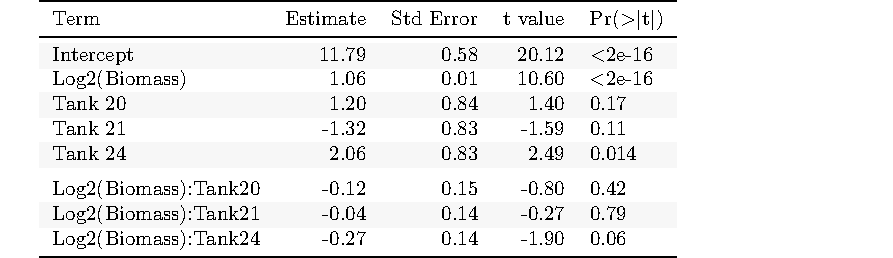
\includegraphics{Chapter3Images/lfulltfac.pdf}
\caption{Parameter estimates and standard errors for the model model, lfull.tfac. This model allowed for interactions between all terms. The $R^{2}$ value is 0.763.}
\label{fig:lfulltfac2}
\end{table}

Table~\ref{fig:lfulltfac2} provides a summary for the full model (lfull.tfac) that includes interactions. We obtain similar estimates to Table~\ref{lab:lmparallel}. However, we now have included interactions. The interaction terms are not statistically significant.  Thus, the interaction between tank and biomass in our modelling is not warranted. This is further evidence that accounting for biomass as a predictor in insolation may be warranted. Notice we obtain identical parameter estimates to those given in Table~\ref{fig:lmedspecific}.

\newpage

We apply ANOVA to compare the current models:

   \vspace{12pt}



\begin{table}[H]
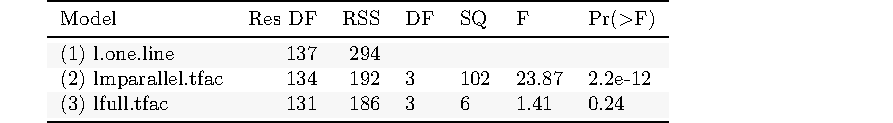
\includegraphics{tablesandimages/anova1.pdf}
\caption{Summary of the additional sum of squares test comparing l.one.line,  lmparallel.tfac and lfull.tfac.}
\label{fig:anovacompare2}
\end{table}


Table~\ref{fig:anovacompare2} provides the results of applying ANOVA on the three previously models. We use an additional sum of squares test to compare the models. We are testing the significance of the three models sequentially. Model 3, lfull.tfac allows for both the slopes and intercepts to change and it also allows for interactions between the terms. Model 2, lfull.tfac, has constant slopes but differing intercepts. Hence the test of model 3 versus model 2 is a test of the hypothesis of a common slope versus different slopes. Since we have a large p-value (0.24), we can conclude that the additional slope parameters are not significantly different from zero. The comparison between model 2 and model 1 is the test of non-differing intercepts for each tank. Because the p-value for this test is so low, we reject this hypothesis. That is, since the p-value (2.2e-12) is so small, we safely reject the null hypothesis (at the 0.05 significance level). Hence, the effect of tank (and hence differing intercepts) is significant and should be included in any modeling. 

\newpage

We now fit a model similar to l.one.line. However, we now collapse over each tank by taking the median value of TCT for each tank. This model is called l.tankregression.med.

   \vspace{12pt}

\begin{figure}[H]
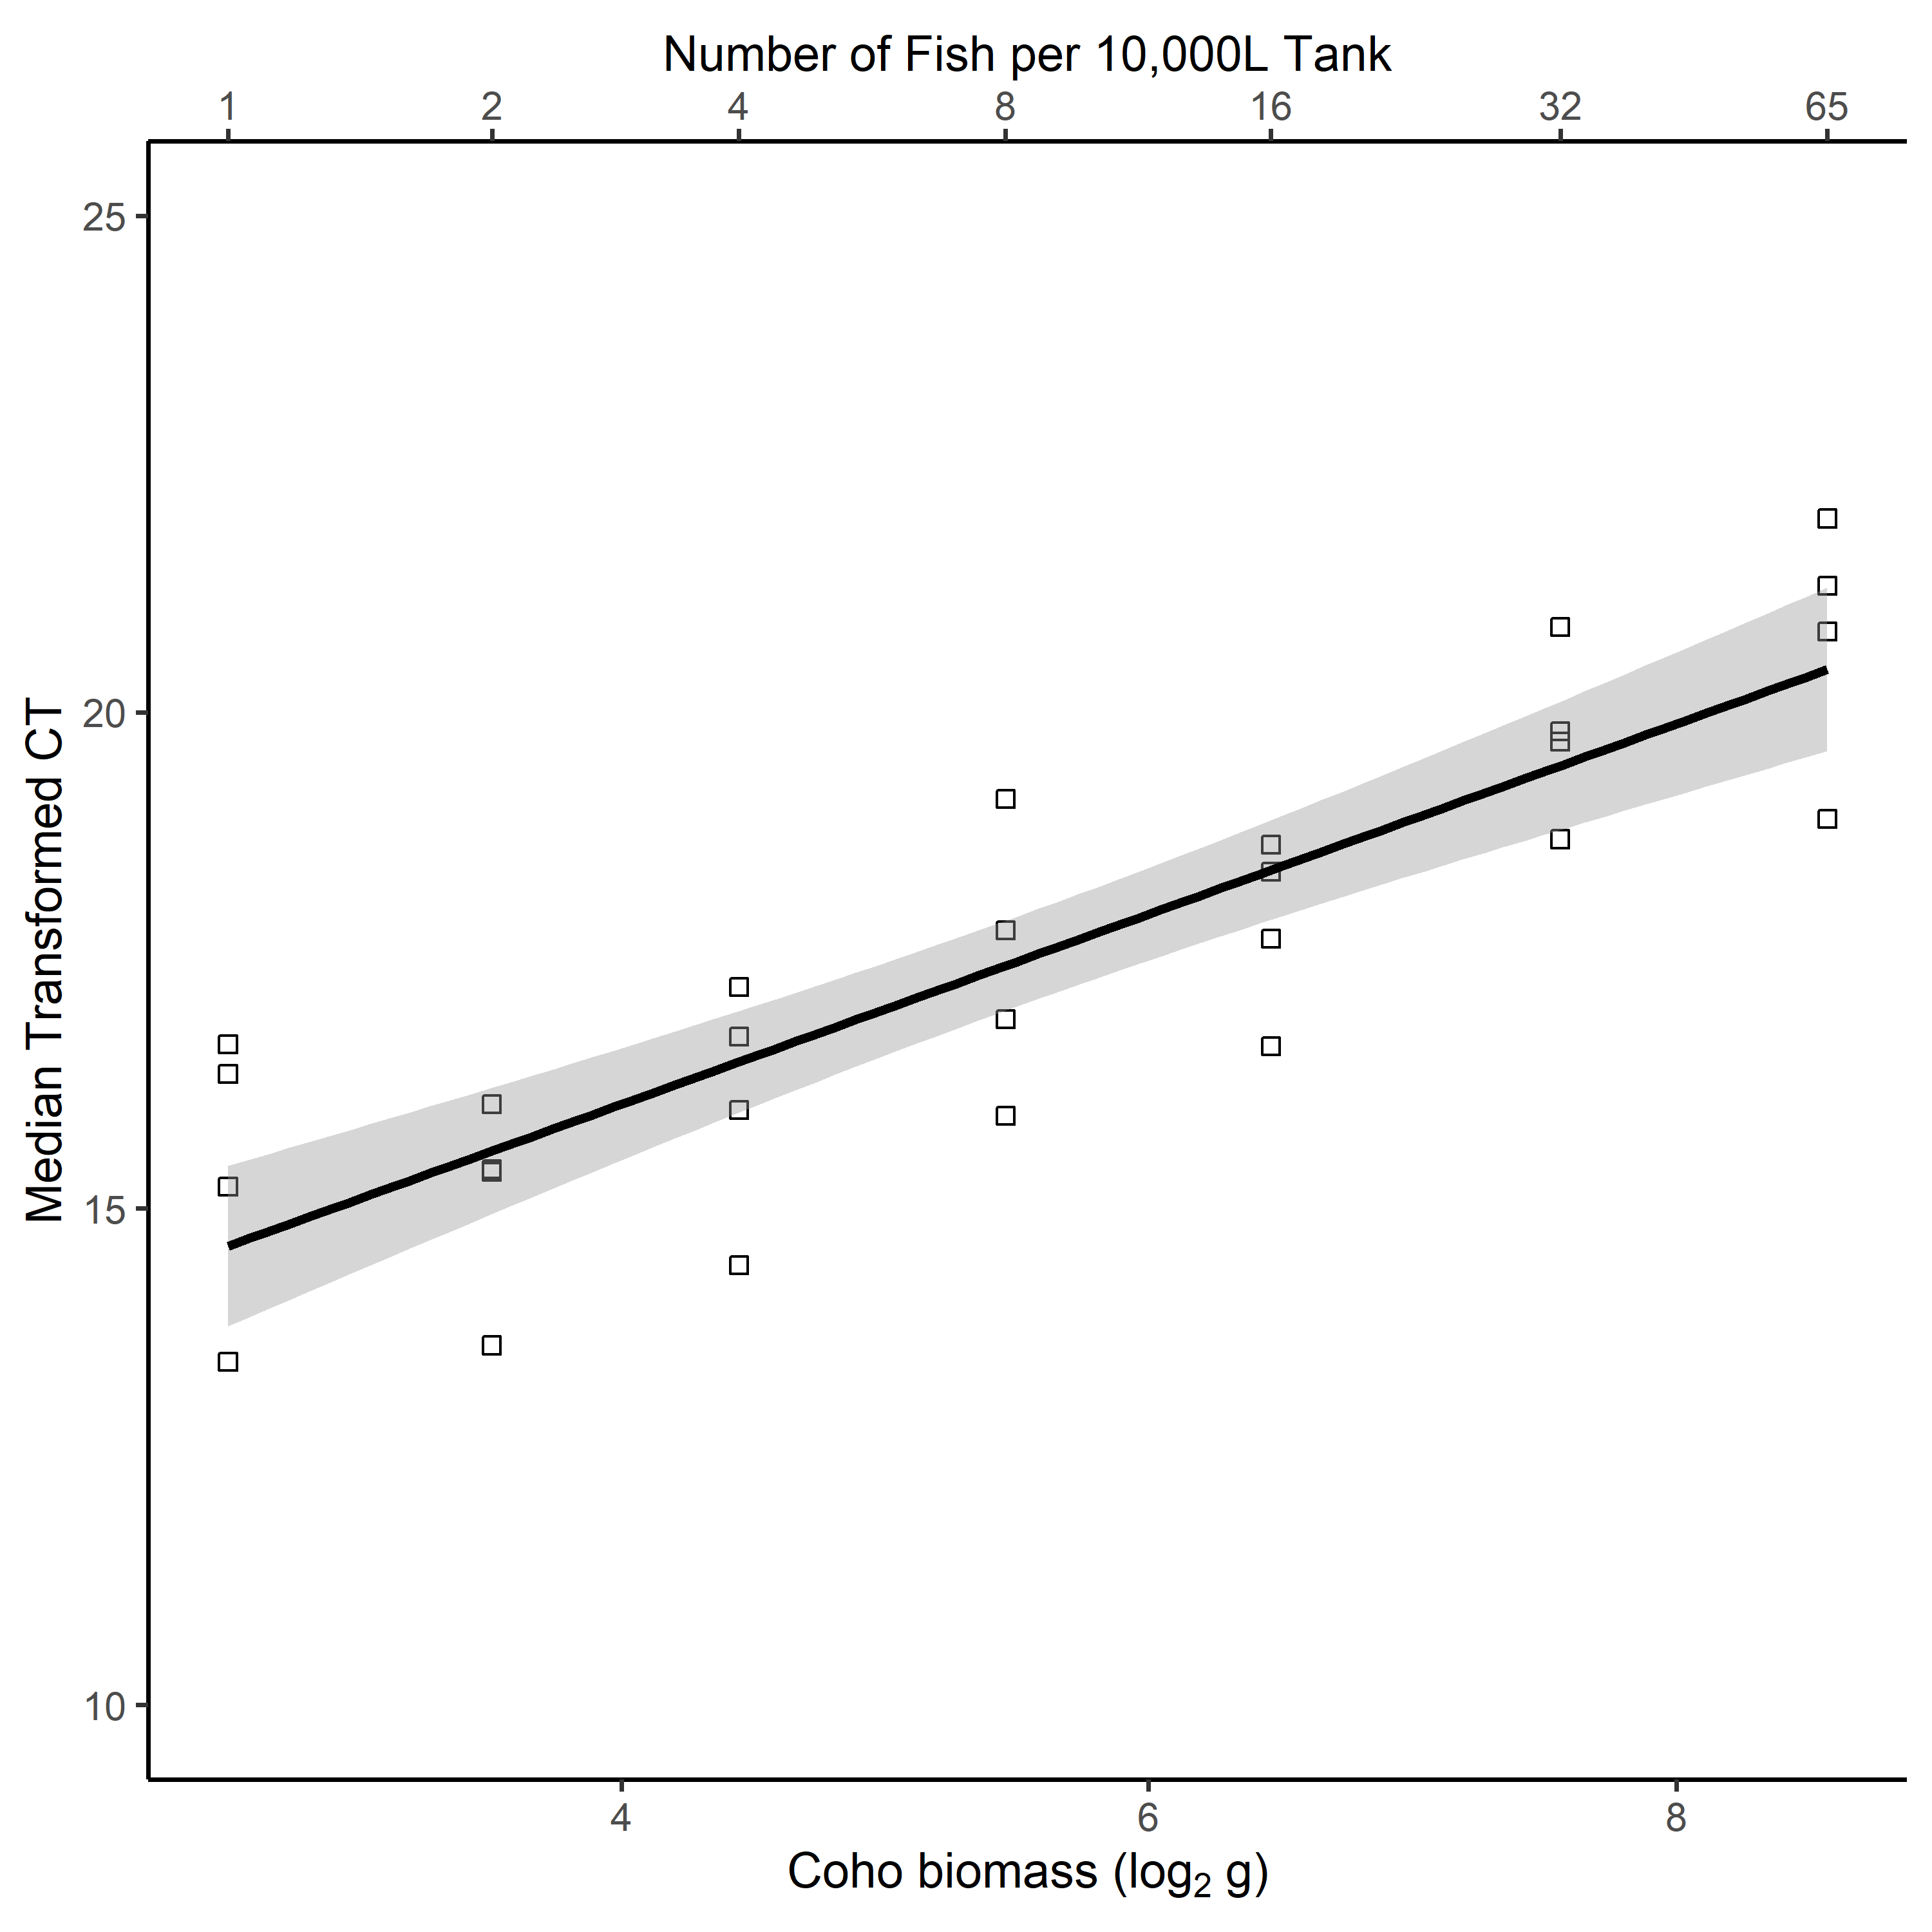
\includegraphics{Chapter3Images/ggplotnew5.png}
\caption{ \hspace{1mm}   Regression line showing the relationship between biomass and Median TCT. Included are the confidence bands about the regression line.  The line is the model l.tankregression.med. The $R^{2}$ is 0.748. Points shown represent the Median TCT for each of the four tanks for each of the seven unique numbers of fish.
}
\label{fig:medct44}
\end{figure}




\begin{table}[H]
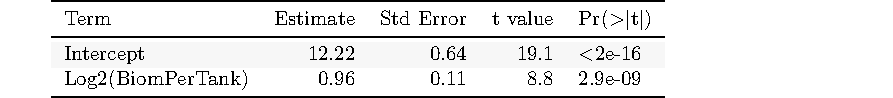
\includegraphics{Chapter3Images/tankregressionMED.pdf}
\caption{Parameter estimates and standard errors for the model l.tankregression.med. This model took the median TCT over each tank for each number of fish. The $R^{2}$ value is 0.748. }
\label{fig:lrankmed}
\end{table}

 Figure~\ref{fig:medct44} is a plot made of our final model, l.tankregression.med. Each point represents the Median TCT for each of the four main tanks. Each distinct biomass value corresponds to a unique number of fish.  The results of this final model are good, as we have quite a large $R^{2}$ value. Table~\ref{fig:lrankmed} summarizes the result of taking the median of TCT over each tank and fitting a simple linear regression model. The only independent variable considered is log2 of Coho biomass. By collapsing over each tank, we were able to capture a large portion of the variation in our data.





\section{Models for Density (Mean)}

We considered modeling the response variable mean TCT. Previously, we considered median TCT. We took an identical approach to the previous models. That is, we first created a simple linear model for predicting the response mean TCT. That is, we created a model l.one.line.mean that only considers Log2(Biomass) as a predictor.

\vspace{12pt}



\begin{figure}[H]
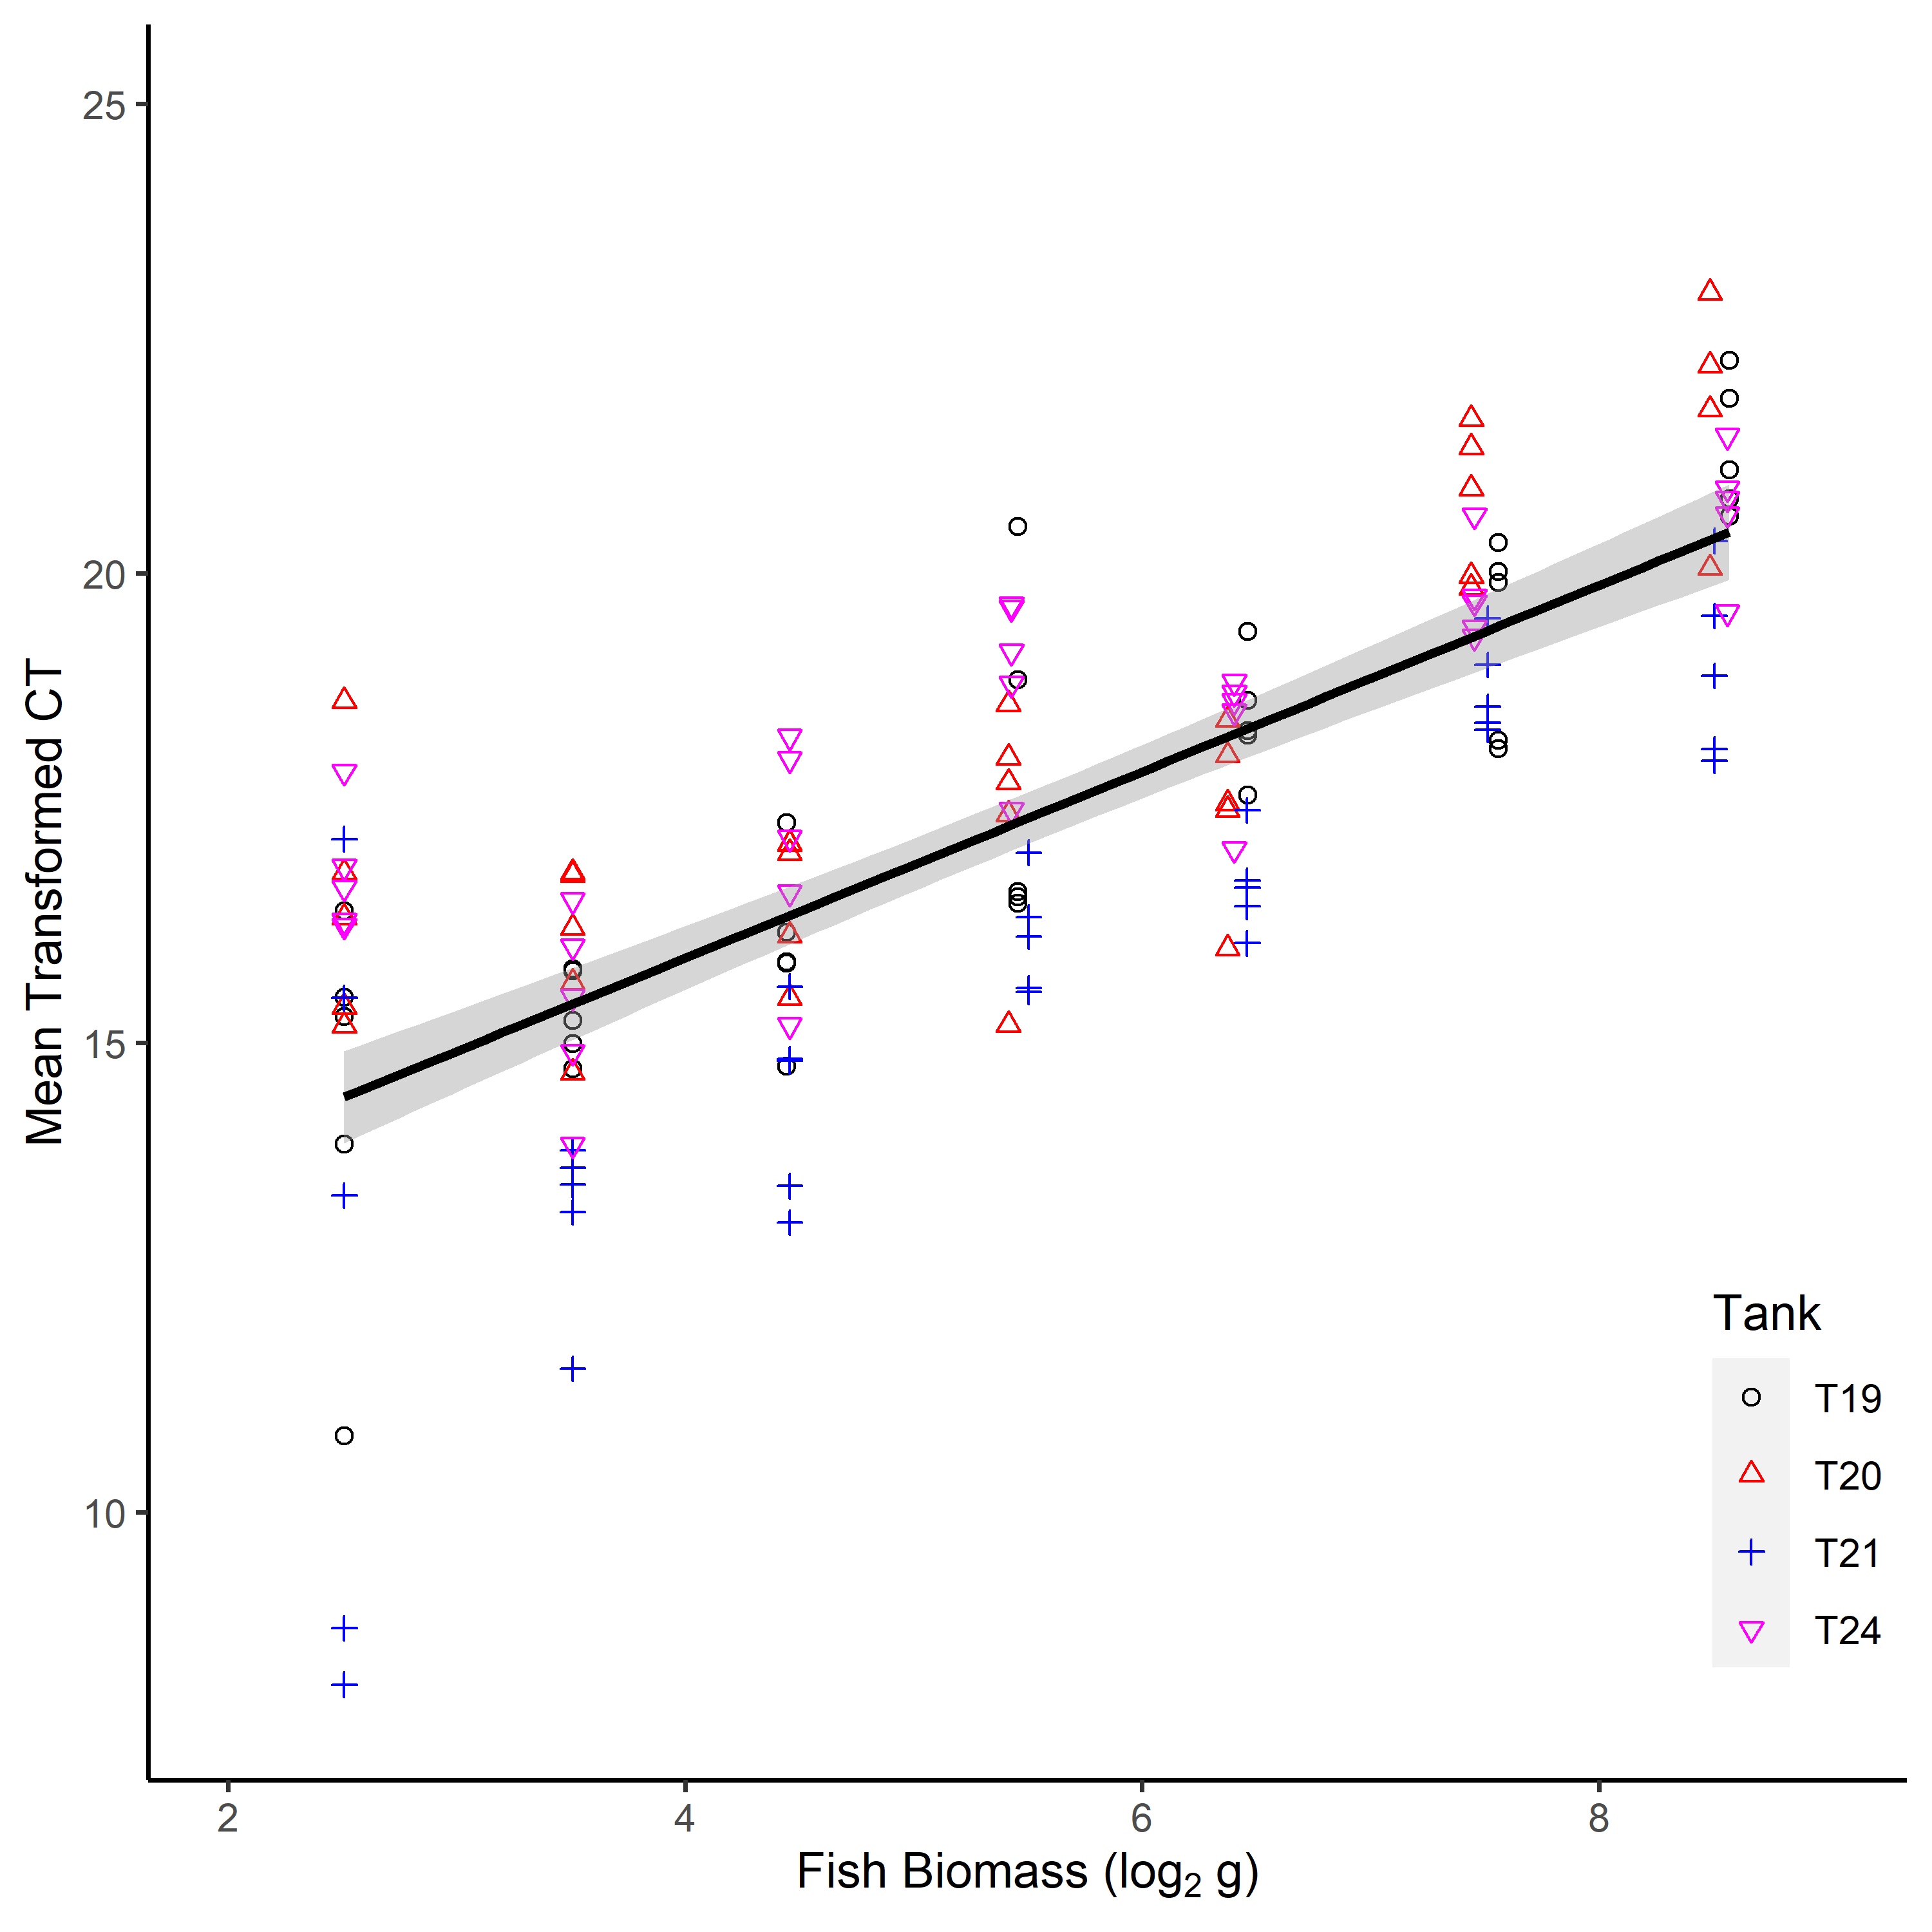
\includegraphics{Chapter3Images/ggplotnew3.png}
\caption{ \hspace{1mm}Mean TCT versus Log2(Biomass). The fitted regression line, l.one.line.mean and the 95 \% confidence intervals are included. Each of the four tanks has an associated color and shape.}
\label{fig:medct3}
\end{figure}

Figure~\ref{fig:medct3} plots l.one.line.mean and the associated 95 \% confidence bands.  Again, we see that the mean TCT from tank 21 tends to be less than the mean TCT from the other three tanks. In general, mean TCT increases as Log2(Biomass) increases.

\vspace{5mm}




\begin{table}[H]
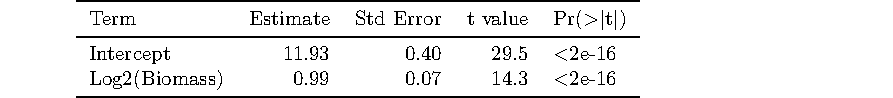
\includegraphics{Chapter3Images/lmMeanCorrect.pdf}
\caption{\hspace{1mm} Parameter estimates and standard errors for the model l.one.line.mean. This is a simple linear regression for mean TCT which only considers Log2(Biomass). The $R^{2}$ value is 0.692.}
\label{lab:loneline.mean}
\end{table}








Table~\ref{lab:loneline.mean} provides a summary of the parameter estimates for the simple linear model, l.one.line.mean. The estimates obtained are very similar to the estimates in Table~\ref{lab:loneline}.

\newpage

Next, we consider a model for mean TCT with biomass as a predictor, and also consider the impact of tank. We first plot regression lines obtained by considering a model with a common slope but allow for differing intercepts.

\begin{figure}[H]
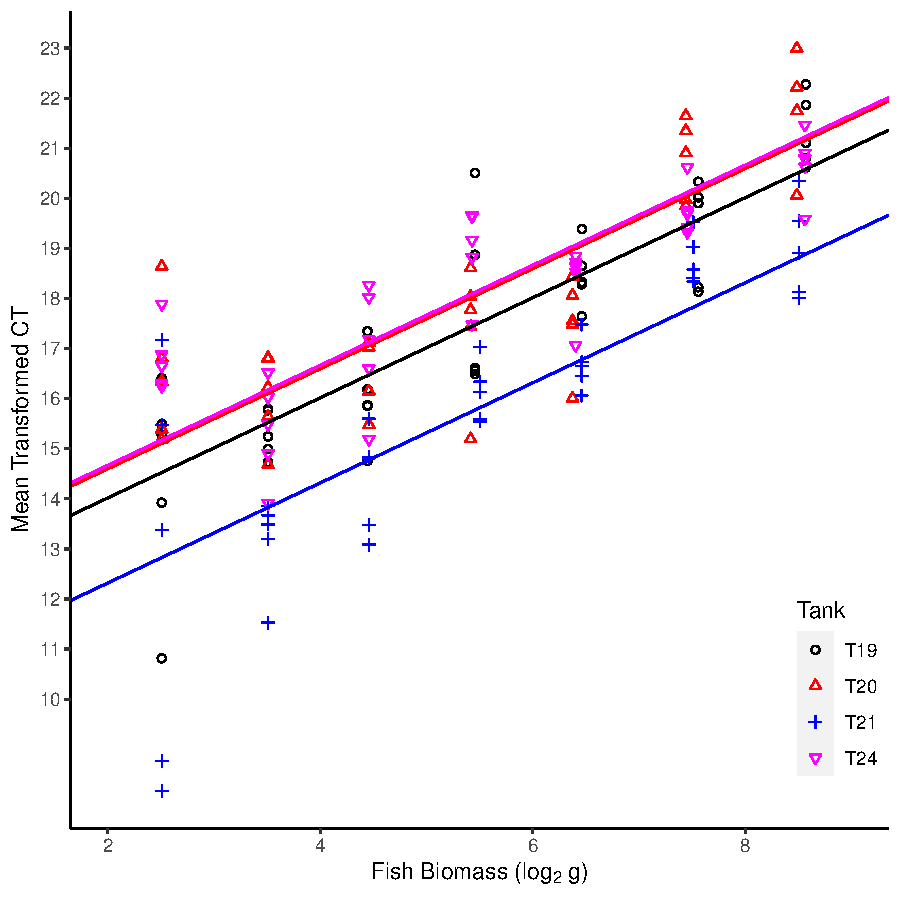
\includegraphics{Chapter3Images/parmean.pdf}
\caption{\hspace{1mm} Lines of best fit by allowing intercept to differ over each tank. This is a plot of the model lmparallel.tfac.mean.}
\label{fig:parmean}
\end{figure}









\begin{table}[H]
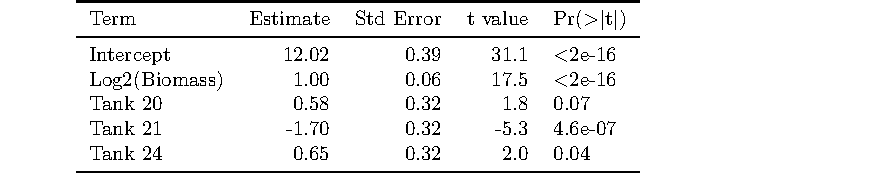
\includegraphics{Chapter3Images/lmMean2.pdf}
\caption{\hspace{1mm}Parameter estimates and standard errors for the model lmparallel.tfac.mean.This model allows for differing intercepts depending on which tank a sample came from. The $R^{2}$ value is 0.735.}
\label{lab:lmparallelmean}
\end{table}


Table~\ref{lab:lmparallelmean} summarizes the result of lmparallel.tfac.mean, which is a model including the tank as a predictor. The estimated intercept is 12.02 for lmparallel.tfac.mean, while the estimated intercept for the median TCT counterpart, lm.tfac was 12.36, which can be seen in Table~\ref{lab:lmparallel}.The effect of tank 21 is highly significant with an estimate of -1.7. That is, tank 21 produces much smaller mean TCT values compared to the other tanks.




\newpage

Finally, we built a full model, lfull.tfac.mean, that includes biomass, tank and the interactions between biomass and tank.

\begin{figure}[H]
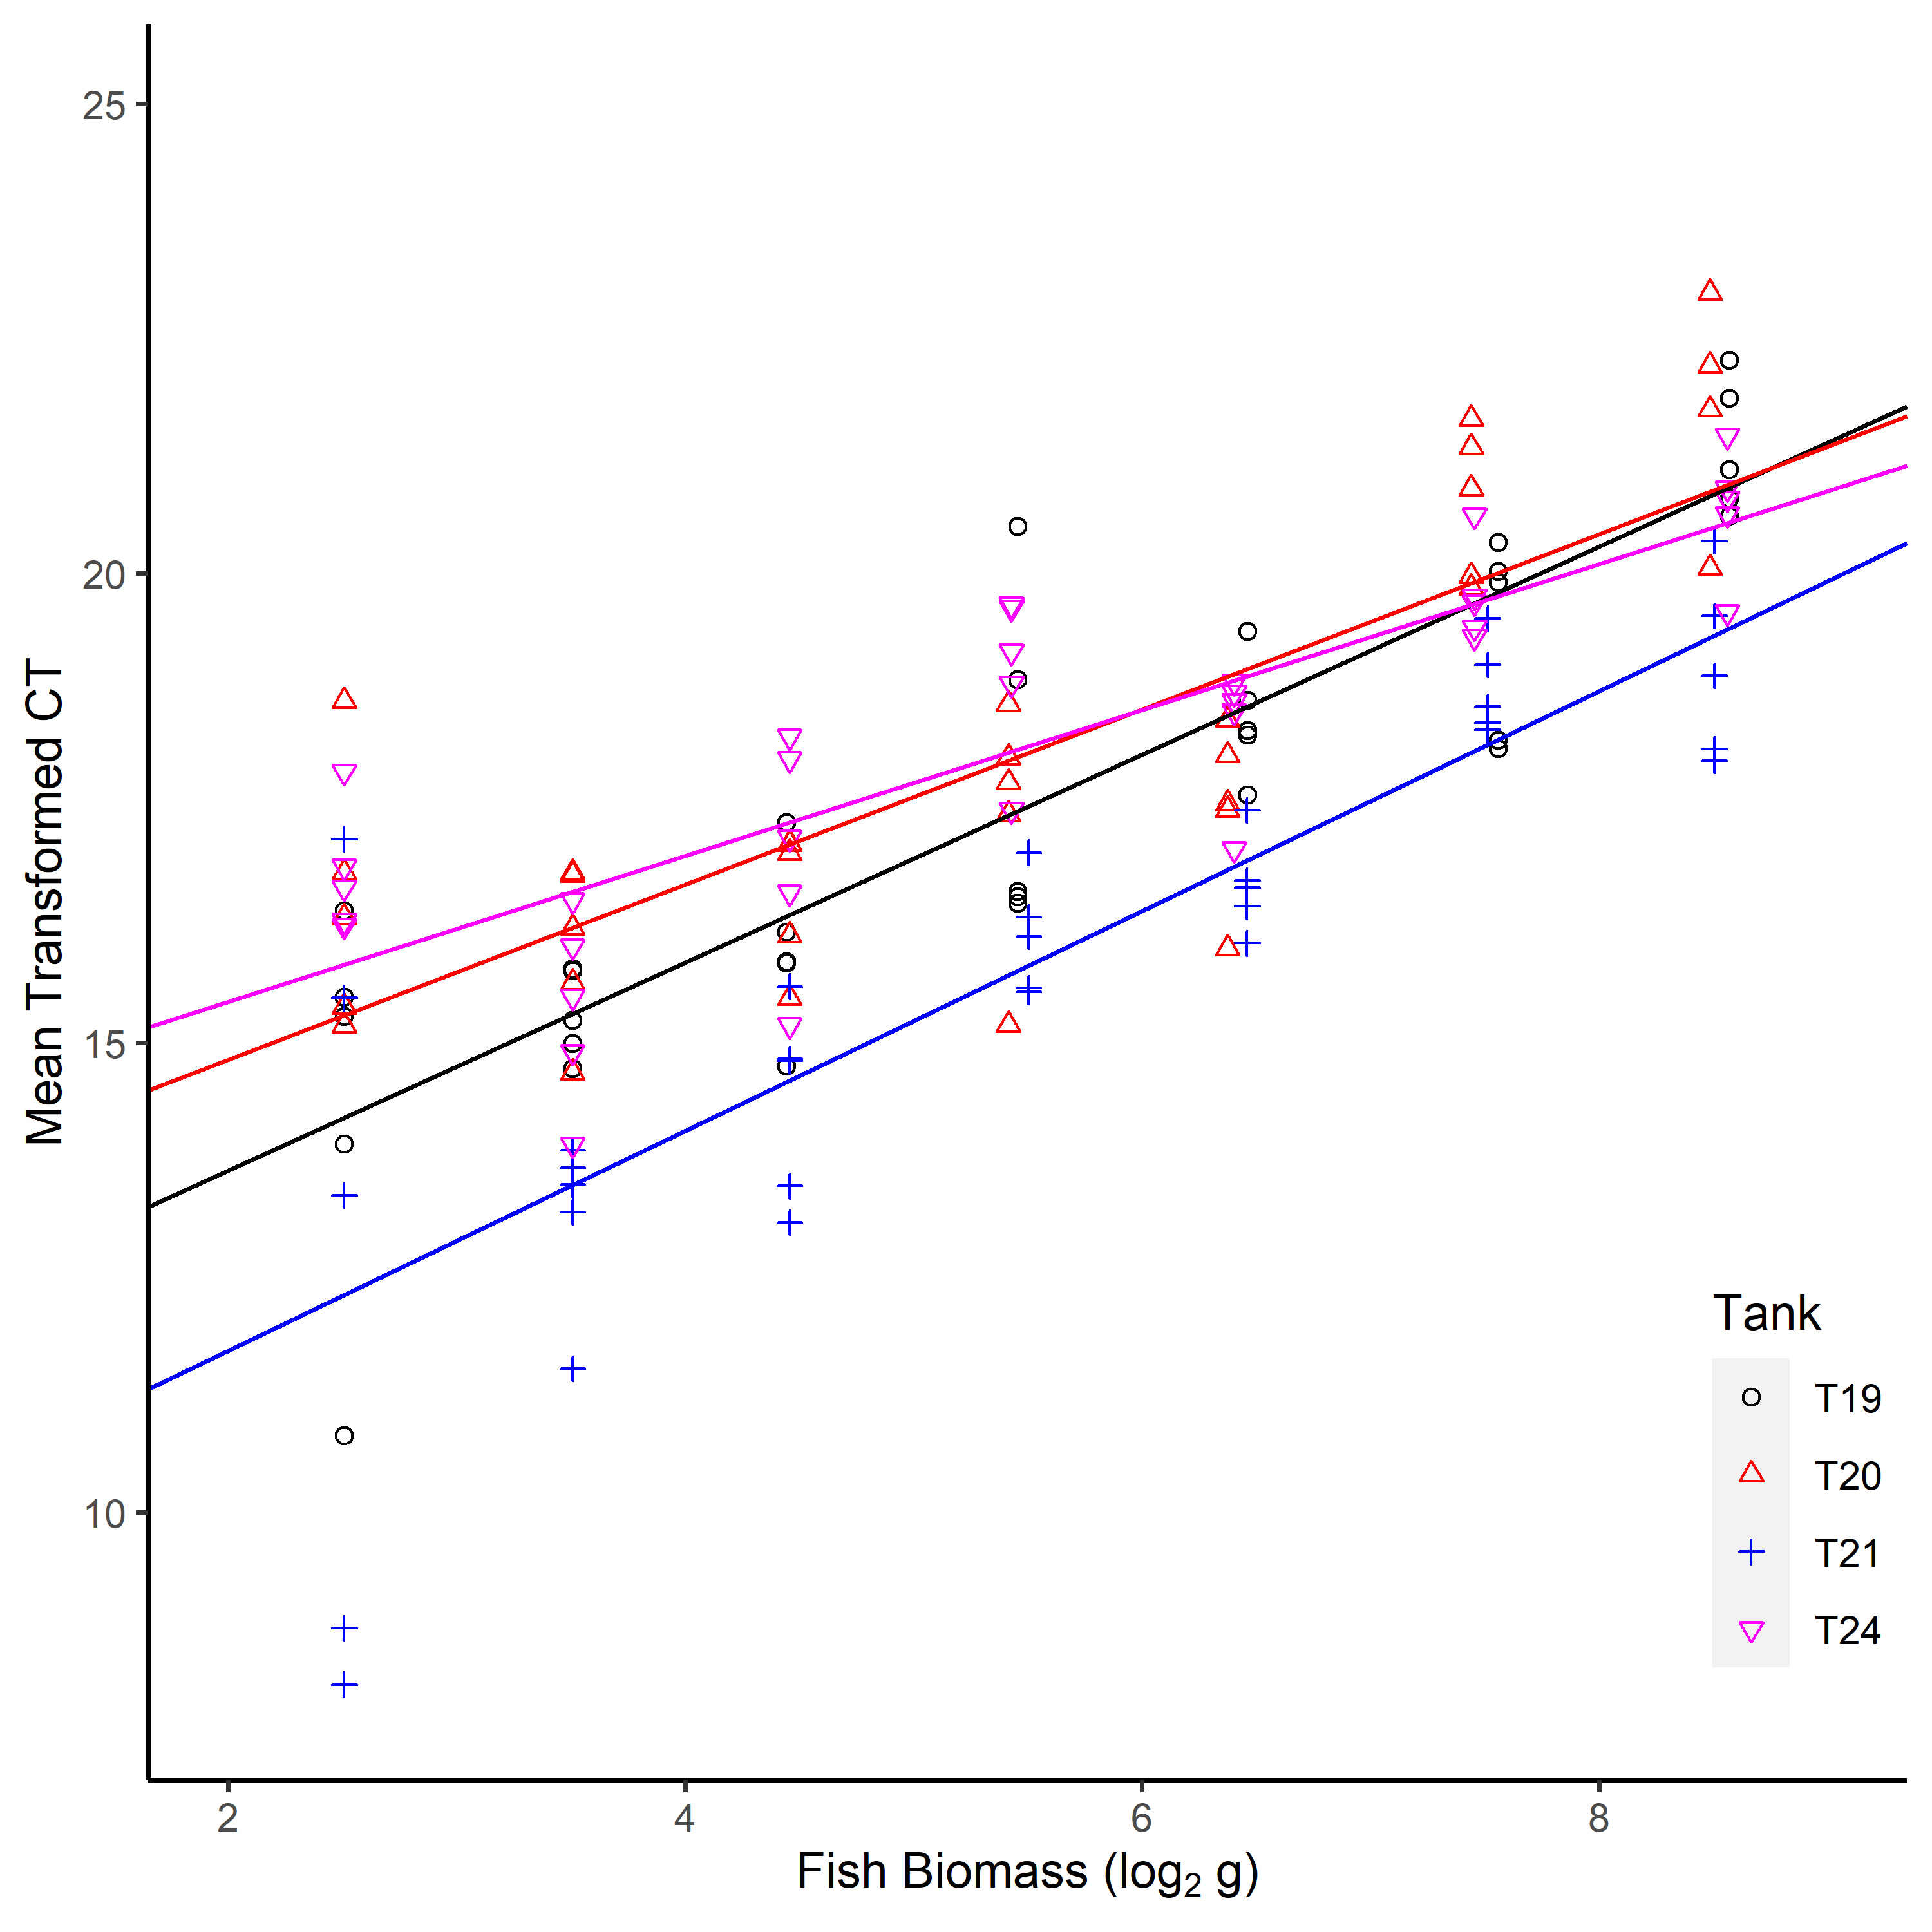
\includegraphics{Chapter3Images/ggplotnew7.png}
\caption{ \hspace{1mm}Lines of best fit by allowing intercept and slope to differ over each tank. This is a plot of the model lfull.tfac.mean.}
\label{fig:parmean}
\end{figure}


\begin{table}[H]
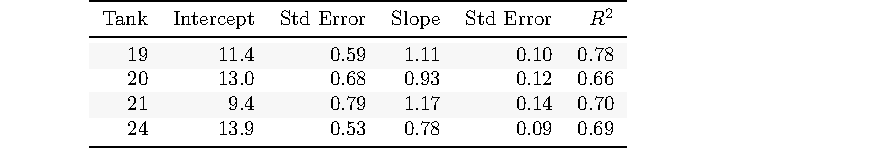
\includegraphics{Chapter3Images/meantankspecific.pdf}
\caption{Table summarizing simple linear regression on Log2(Biomass) when each tank is considered in isolation for mean TCT.}
\label{lab:sepmean}
\end{table}


Table~\ref{lab:sepmean} summarizes the results of applying simple linear regression to each tank in isolation. We obtained separate estimates for each intercept and slope. Tank 21 has the smallest intercept, while tank 24 has the largest intercept. The slopes are similar; however, tank 24 has a noticeably smaller slope. The $R^{2}$ are all quite high, but tank 19 alone has the highest $R^{2}$.







\begin{table}[H]
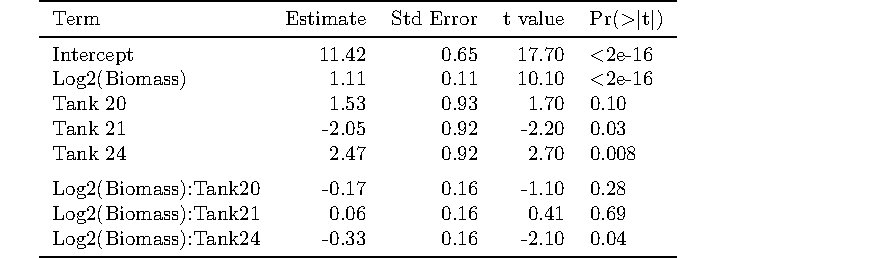
\includegraphics{Chapter3Images/lmMean3.pdf}
\caption{ \hspace{1mm}Parameter estimates and standard errors for a model that includes Log2(Biomass), tank and the interaction between tank and Log2(Biomass). Model:  lfull.tfac.mean. The $R^{2}$ value is 0.75.}
\label{fig:lfull2}
\end{table}


Figure~\ref{fig:parmean} is the plot of the model  lfull.tfac.mean. The intercept and slope is allowed to vary over each tank. Table~\ref{fig:lfull2} provides the summary of  lfull.tfac.mean. For the full model with mean TCT as the response and  both tank and the interaction between tank and biomass as predictors, the least squares estimate of the intercept term is 11.42. For the full model on median TCT, the least squares estimate of the intercept is 11.79. This model provides identical results to considering each tank in isolation, as seen by comparing the estimates to those given in Table~\ref{lab:sepmean}.

\newpage

We again create an ANOVA table:

   \vspace{12pt}




\begin{table}[H]
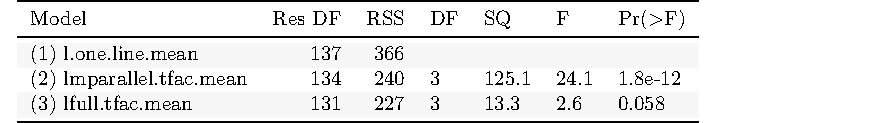
\includegraphics{Chapter3Images/anovamean.pdf}
\caption{\hspace{1mm}Summary of the additional sum of squares test for the Mean TCT models. }
\label{fig:anovamean11}
\end{table}


 
 Table~\ref{fig:anovamean11} shows the results of applying an ANOVA (additional sum of squares test) on the three models for Mean TCT. The interpretation is the same as it was with the anova table for median TCT. Since lmparallel.tfac.mean has a very small p-value, we conclude that we need to include the tank effect in our model (that is, we reject the hypothesis that differing intercepts is zero). 
Since the p-value associated with  lfull.tfac.mean is 0.058; this indicates that including interaction for modelling mean TCT is marginally significant (at the 0.05 level). The $R^{2}$ for lmparallel.tfac.mean is 0.735 while the $R^{2}$ for  lfull.tfac.mean is 0.750. Although the $R^{2}$ increases, it is only by a small amount. Since the p-value is on the boundary of significance, we may still choose to ignore the interaction term as it adds complexity and only slightly increases the $R^{2}$.

\newpage


We now fit a model similar to l.one.line.mean. However, we now collapse over each tank by taking the mean value of TCT. This model is called l.tankregression. Note this predictor, Log2(BiomassTank), is the Log2 taken over total weight in each of the four tanks.

 
\begin{figure}[H]
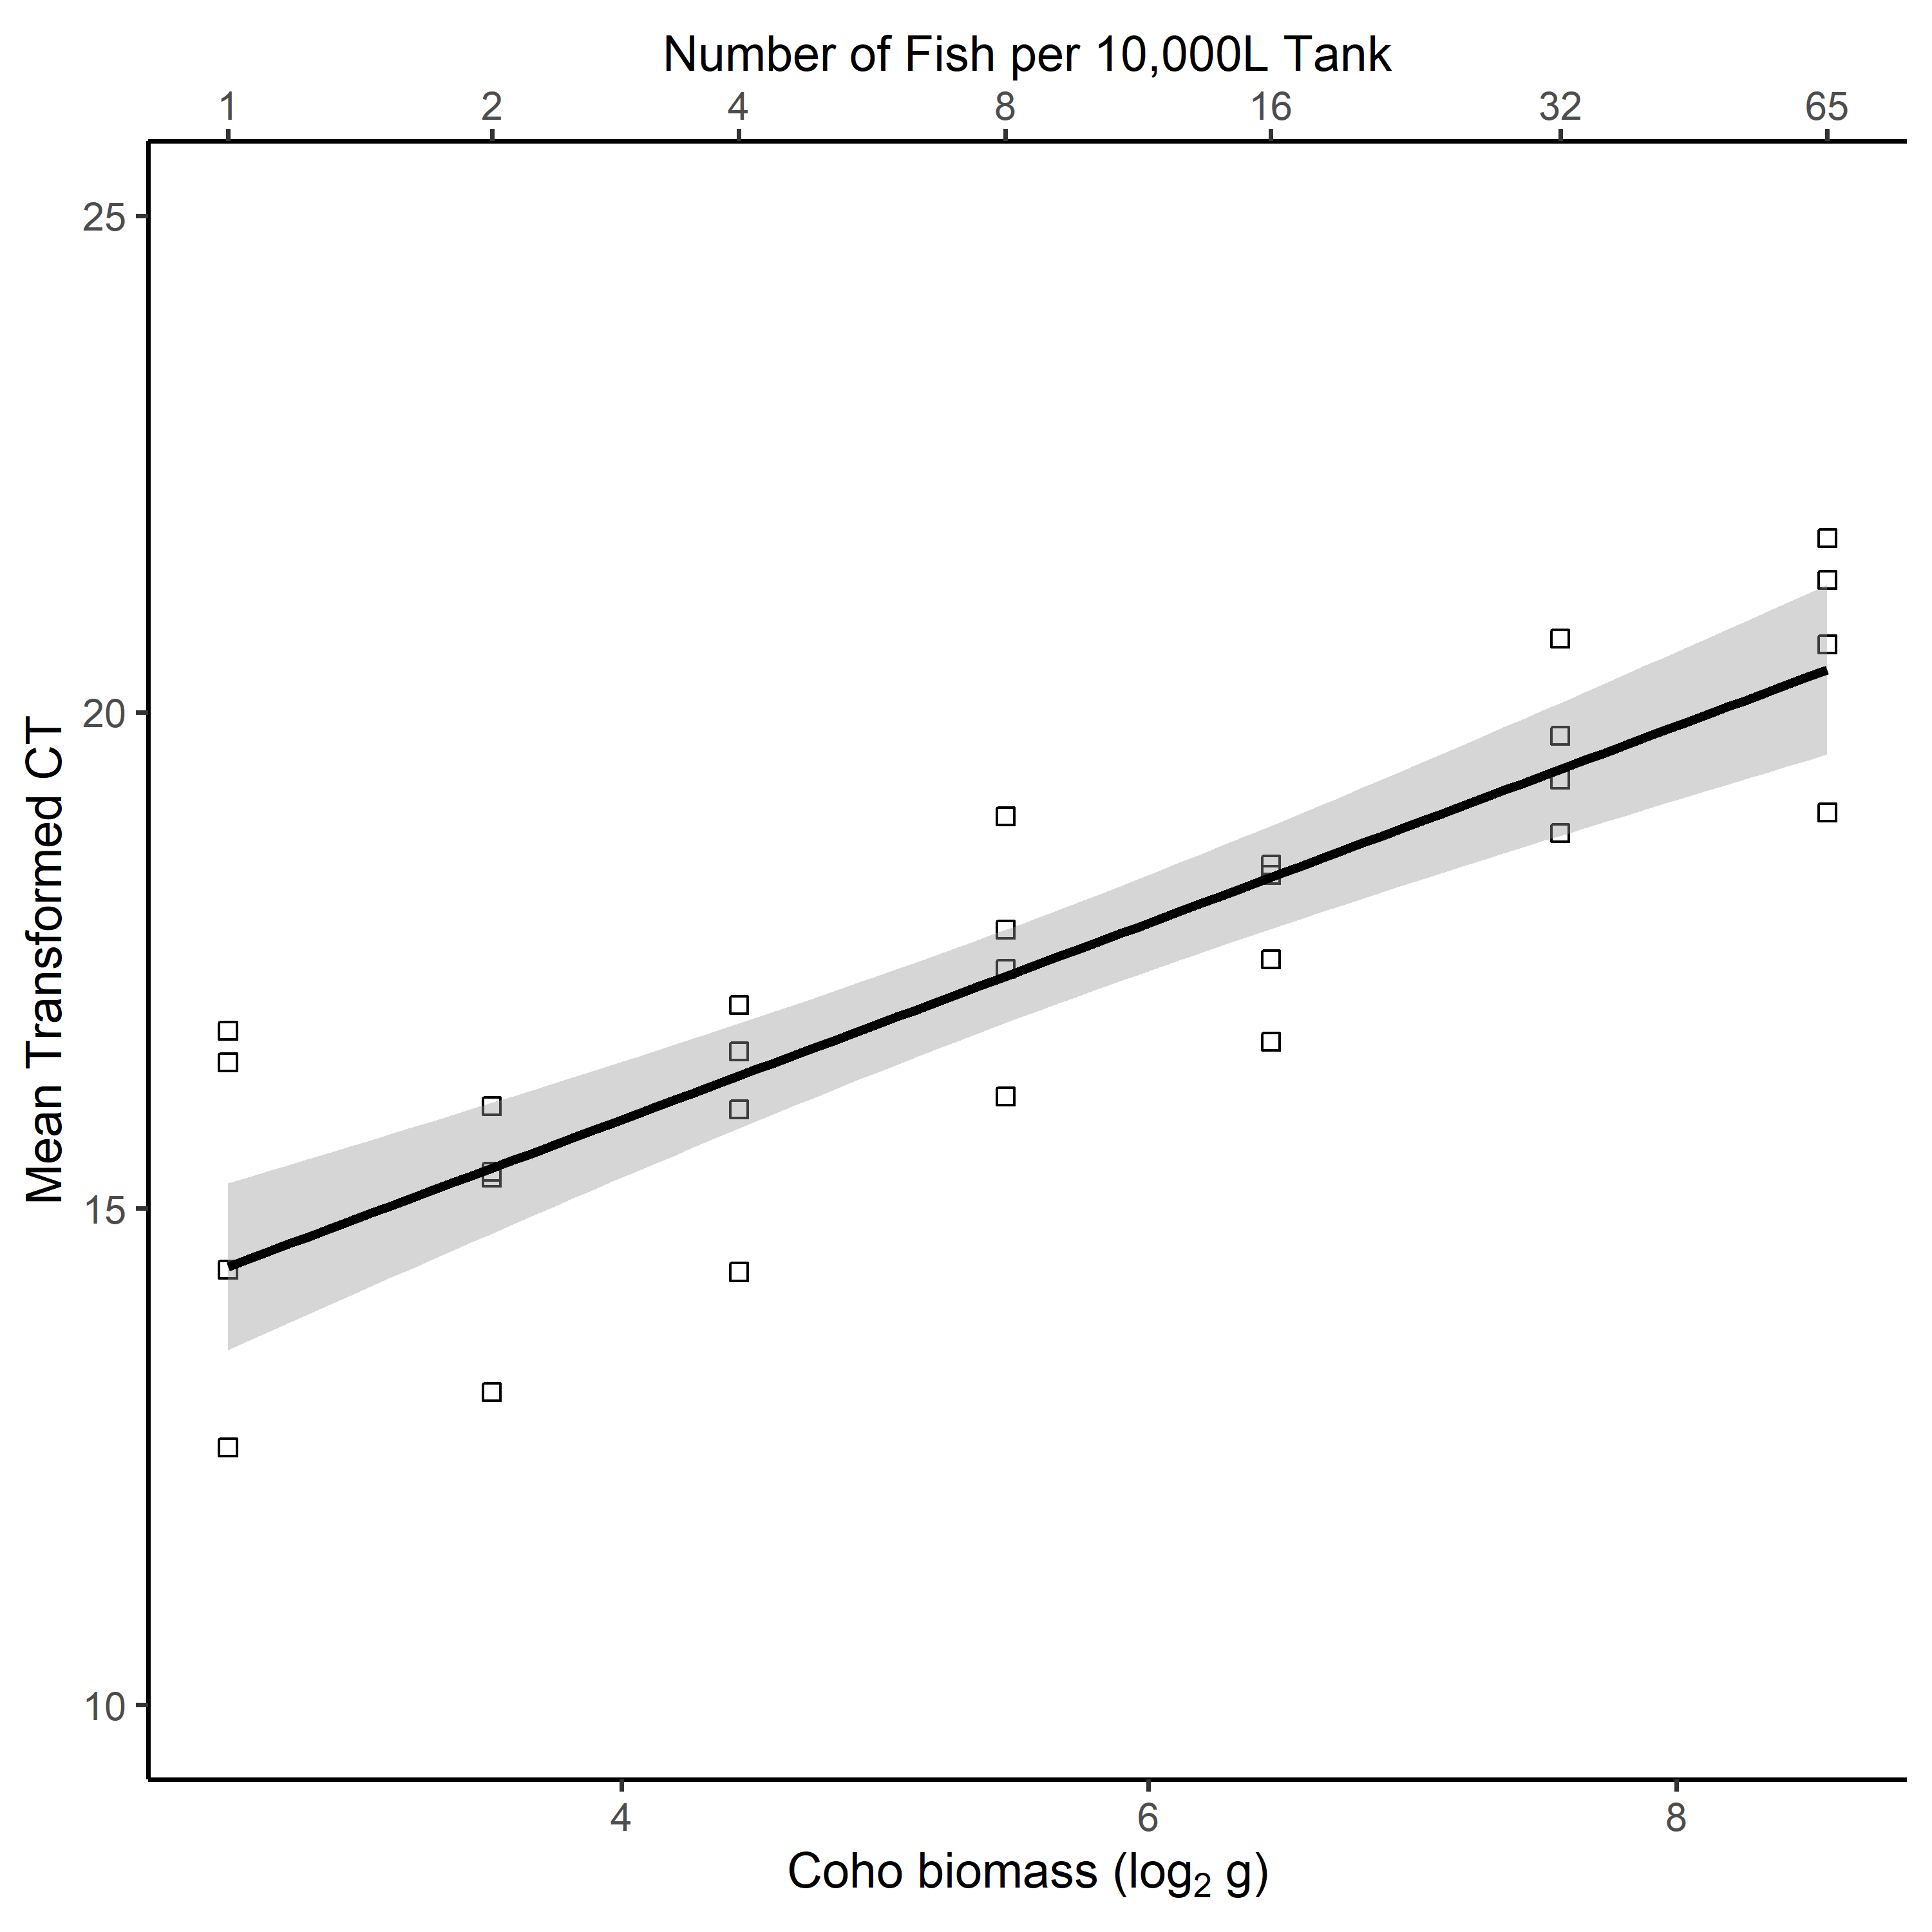
\includegraphics{Chapter3Images/ggplotnew4.png}
\caption{ \hspace{1mm} Regression line showing the relationship between Mean TCT and biomass. Included are the confidence bands about the regression line.  The line is the model l.tankregression. The $ R^{2}$ is 0.748. Points shown represent the Mean TCT for each of the four tanks for each of the seven unique numbers of fish.
}
\label{fig:medct55}
\end{figure}



\begin{table}[H]
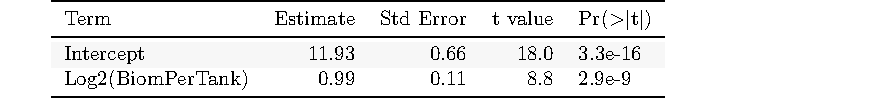
\includegraphics{Chapter3Images/tankregressionMEAN.pdf}
\caption{\hspace{1mm}Parameter estimates and standard errors for model: l.tankregression. The $R^{2}$ value is 0.748.}
\label{fig:lrankmean}
\end{table}

Table~\ref{fig:lrankmean} summarizes the result of taking the mean of TCT over each tank and fitting a simple regression model. The only variable considered is the Coho biomass. Figure~\ref{fig:medct55} is the regression line obtained by applying simple linear regression over the points collapsed by taking the mean over each tank. The $R^{2}$ is high, indicating our model does a good job at explaining variation in the data. Moreover, it has a simple interpretation (Mean TCT increases linearly with Log2(Biomass) and thus reduces complexity.




Figure~\ref{fig:medct55} is a plot made of our final model. Each point represents the Mean TCT for each of the four main tanks. Each distinct biomass value corresponds to a unique number of fish. 



\section{Robust Models}

We model using a robust fit from the `robust' package, and the lmRob function \citep{RobustModels}. This fits a `robust model' which is less sensitive to outliers than a regular least squares, linear fit. The function lmRob automatically chooses an appropriate algorithm to efficiently fit a model.  The default fitting method is the so called `data-dependent algorithm'.

 \vspace{12pt}

 Again, we used median TCT as our response variable. Initially, we fit a simple robust model, lr, to our response variable, Median TCT, with  a single input predictor, Log2(Biomass). Next, we fit two multiple linear models. lrparallel.tfac is a multiple linear model with the two predictors Log2(Biomass) and tank. Finally, we fit  lrfull.tfac, that incorporates both Log2(Biomass) and tank as well as the interaction between Log2(Biomass) and tank. 

 \vspace{12pt}




\begin{table}[H]
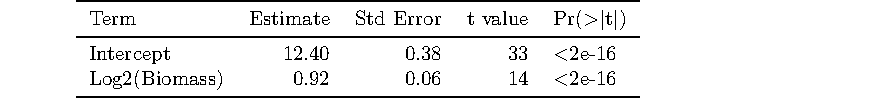
\includegraphics{Chapter3Images/robust1.pdf}
\caption{\hspace{1mm}Parameter estimates and standard errors for our simple robust model: lr. The $R^{2}$ value is 0.546.}
\label{fig:robust1}
\end{table}

 Table~\ref{fig:robust1} provides the results of fitting a simple linear model for median TCT using lmRob. For a unit increase in Log2(Biomass) this model predicts an increase in 0.925 for median TCT. This also makes sense, as Log2(Biomass) increases, we expect that the volume of eDNA in the tank will increase, and hence CT will decrease (and TCT will increase).The p-value for both intercept and Log2(Biomass) are extremely low, indicating that both  play an important role in the model. The estimates for the intercept in both the robust and linear model are quite similar.  The estimate for Log2(Biomass) is slightly less for the robust fit. We then fit a robust model for median TCT that includes biomass as a predictor and also considers tank as a possible predictor.

 \vspace{12pt}




\begin{table}[H]
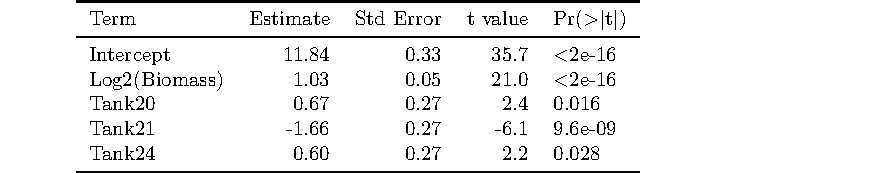
\includegraphics{Chapter3Images/robust2.pdf}
\caption{\hspace{1mm}Parameter estimates and standard errors for the model lrparallel.tfac. The $R^{2}$ value is 0.619.}
\label{fig:robust2}
\end{table}



Table~\ref{fig:robust2} summarizes the model lrparallel.tfac.  For this model, lmRob produces similar conclusions for both the intercept and for the Log2(Biomass).   However, we now also have estimates for the tank. The data indicates that compared to the baseline of tank 19, tank 20 and 24 produce slightly higher median TCT estimates, while on the other hand Tank 21 produced lower TCT. These differences are possibly due to differences in bleaching and cleaning of the tanks.

 \vspace{12pt}

Finally, we fit a robust model (lrfull.tfac) for the response median TCT that includes biomass, tank, and the possible interactions between biomass and tank.

\vspace{12pt}



\begin{table}[H]
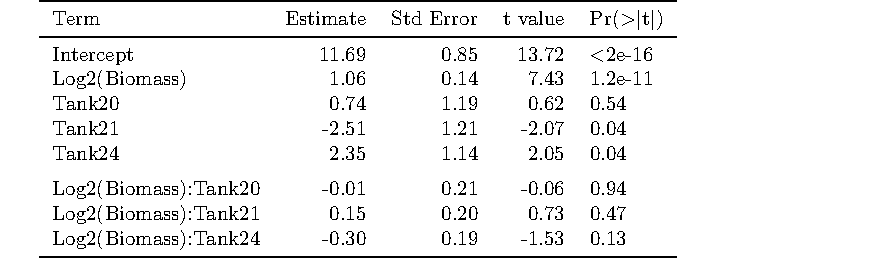
\includegraphics{Chapter3Images/robust3.pdf}
\caption{\hspace{1mm}Parameter estimates and standard errors for the model lrfull.tfac. The $R^{2}$ value is 0.649.}
\label{fig:robust3}
\end{table}

 \vspace{12pt}

Table~\ref{fig:robust3} summarizes the estimates of lrfull.tfac. The robust model, lrfull.tfac containing Log2(Biomass), tank and their interaction terms produces similar results to lrparallel.tfac.
 The multiple $R^{2}$ for this model is only slightly larger than lrparallel.tfac at 0.649. The interaction terms between tank and Log2(Biomass) are not significant.  We confirmed this with an `anova' test (additional sum of squares) using the built in R function. 
  
\vspace{12pt}


 Recall that anova compares a variety of nested models. Our first model is lr, which included Log2(Biomass). Our second model, lrparallel.tfac includes for Log2(Biomass) and tank. 
 



\begin{table}[H]

\includegraphics{Chapter3Images/robustanova.pdf}
\caption{\hspace{1mm}Table of results for comparing the robust models using a Robust ANOVA.}
\label{fig:robustanova}
\end{table}

Table~\ref{fig:robustanova} is the results of applying an anova test to our robust models. We do not reject the hypothesis (at the 0.05 significance level) that the interaction term is zero. We do reject the null hypothesis that the tank term is zero.
















\section{Residual Analysis}

We now consider the residuals for some of the models we previously fit. To create the residual plot for l.tankregression we used the `broom' package \citep{broom}.


\begin{figure}[H]
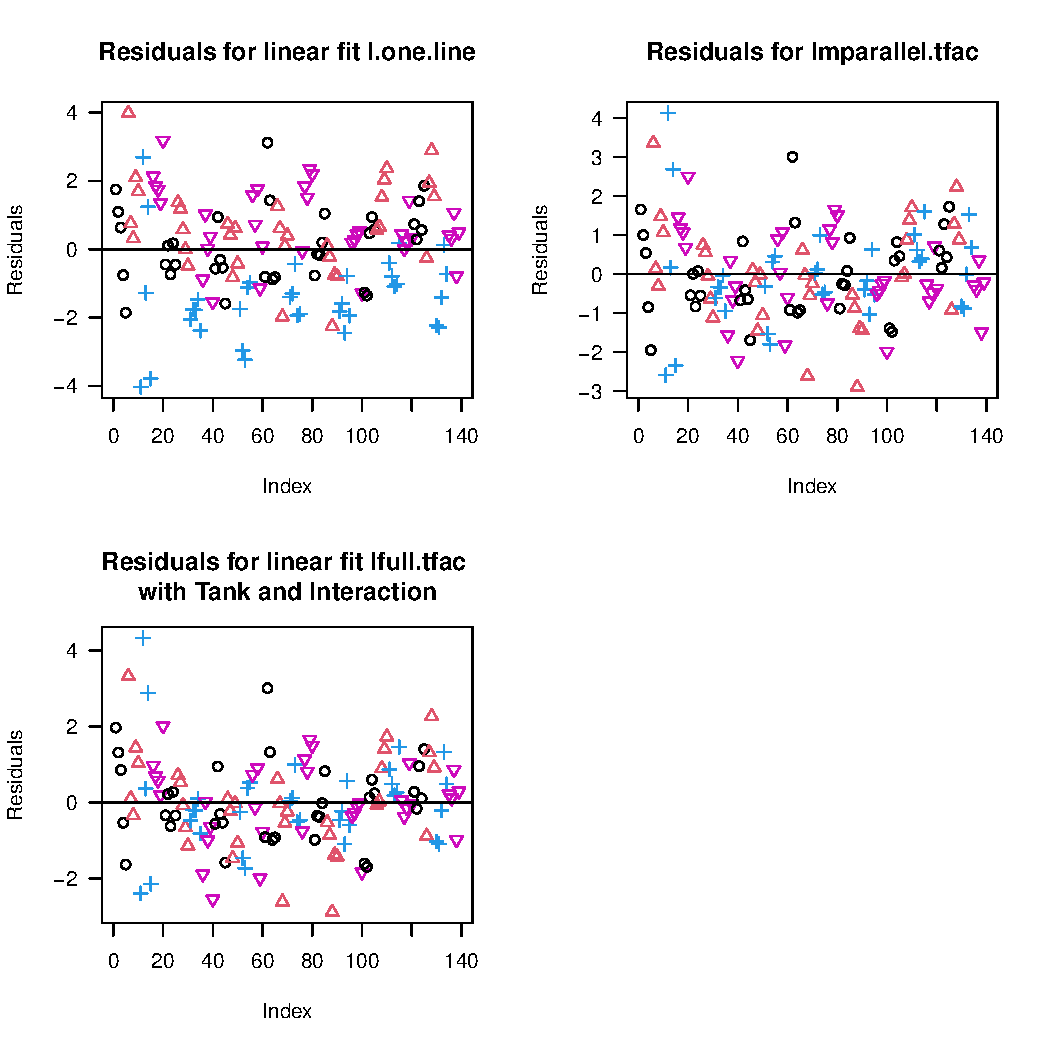
\includegraphics[scale=0.9]{Chapter3Images/residuals2.pdf}
\caption{ \hspace{1mm} Residual plots for three models, l.one.line, lmparallel.tfac and lfull.tfac are the standard linear models for median TCT. Tanks 19, 20, 21 and 24 are represented as black circles, red triangles, blue crosses and pink inverted triangles respectively. }
\label{lab:resid2}
\end{figure}



\begin{figure}[H]
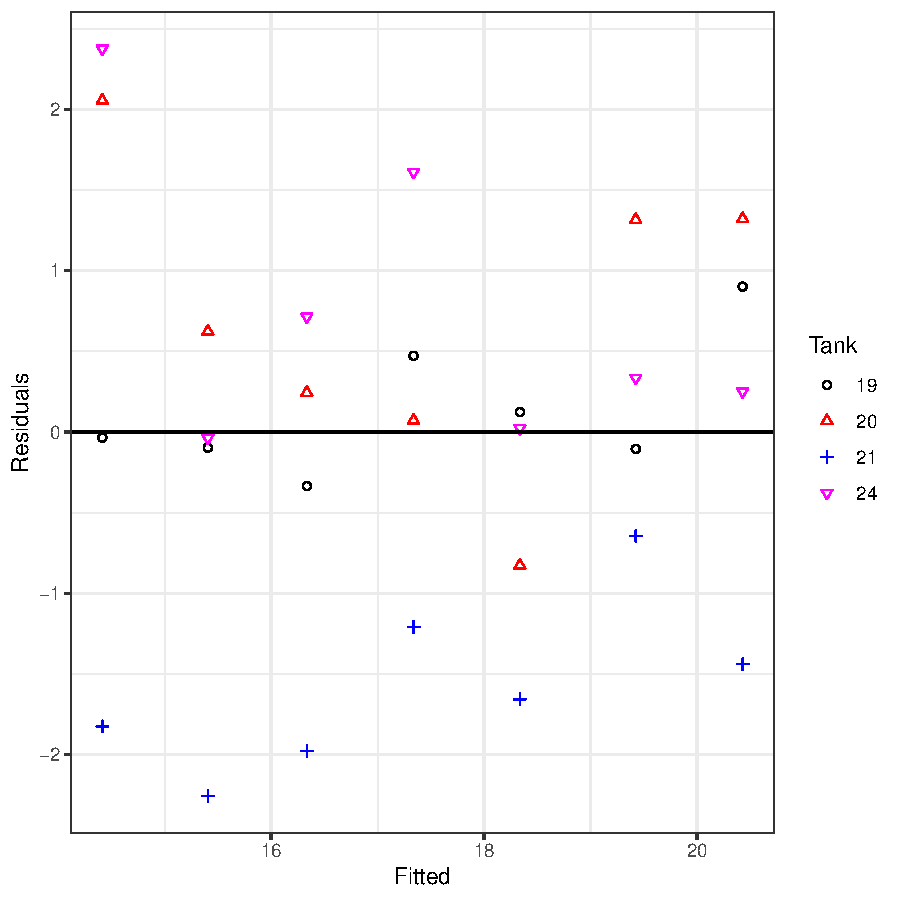
\includegraphics{Chapter3Images/ltankregressionresid.pdf}
\caption{\hspace{1mm} This image shows the residuals versus the fitted values for our final chosen model for mean TCT, l.tankregression.}
\label{lab:resid22}
\end{figure}

Figure~\ref{lab:resid2} shows the residuals from three of the models we fit. The residuals appear to be randomly distributed about the x-axis which is a good indication that our model is making valid assumptions. Figure~\ref{lab:resid22} is a plot of the residuals for l.tankregression. The residuals again appear to be randomly distributed about the x-axis. Although Tank 21 has consistently negative residuals. The legend indicates which tank each point belonged to.




\startchapter{Conclusions and Future Work}
\label{chapter:Conclusions}

\section{Overview}

This research and analysis brought together the disciplines of statistics, biochemistry, microbiology and genetics to provide further validation of several key concepts regarding environmental DNA.  


\vspace{5mm}
In the density experiment, varying numbers of Coho salmon were placed in large tanks and water samples were collected after allowing some time for the fish to swim in the tanks. Water samples were stored and transferred to the lab where they were tested for DNA integrity. Samples that passed integrity tests were then analyzed using Real-time polymerase chain reactions. This process used a thermal cycler to monitor the amplification of  Coho specific target DNA. Detection of target DNA in the thermal cycler results in the release of fluorescence, visible to the researcher. When target molecule concentrations are very low, we expect that we will need several `cycles' in order to detect the DNA (and hence several cycles needed to produce fluorescence). On the other hand, when target DNA is highly concentrated, we expect many less cycles to detect DNA. The number of cycles taken to produce fluorescence is referred to as the Cycle threshold, or simply `CT'. We chose to work with a monotone transformed version, TCT which was simply 50-CT. TCT should always be positive, as beyond 50 cycles is equivalent to a `non-detection'.

\vspace{5mm}
Using the transformed CT (`TCT') values obtained via qPCR, we established a significant relationship between Coho biomass and detectable eDNA. This experiment confirmed what we would expect, as clearly more or larger fish would be expected to shed or release more DNA into their environments. One highlight of this experiment is a figure that summarizes many concepts into a clear and concise manner, Figure~\ref{fig:medct55}. This figure showed a strong relationship between the number of fish in a tank and the mean TCT measurements obtained. The $R^{2}$ for the model was nearly 0.75, indicating the model explained much of the variation in the dataset. Residual analysis was conducted that provided further validation that the models were performing well.

\vspace{5mm}

The second experiment we analyzed was the `dilution' experiment.  In this experiment, three juvenile Coho salmon were again placed in large tanks and left to equilibrate for several days. The fish were then removed, and samples were taken as the tank water drained and was replaced by fresh water (via an inflow pipe). We found that instead of a linear relationship, a more sophisticated model was needed. In particular, we needed a model that accounted for the point in which the water was completely diluted (the so called `breakpoint'), where qPCR no longer detected any eDNA. 
\vspace{5mm}

Still water ponds or lakes are only a fraction of all bodies of water. In reality, researchers will be taking measurements from all sorts of water systems, including those with strong currents and fast flows. We confirmed that increased flow rates result in lower amounts of detectable eDNA in the experiment. We were able to fit several niche models to explain the impact of flow on our TCT measurements. In the end we had success fitting a bent cable model, Figure~\ref{fig:bentcablemean} that captured much of the variation in the dataset.

\vspace{5mm}

The last set of data analyzed was actual field data obtained from several streams in British Columbia. Here we attempted to use what was found in the first two experiments (the impact of biomass and flow) to study these streams. 

\vspace{5mm}

In addition, the field data allowed us to implement covariate analysis, whereby we were able to `tease' out the most important factors impacting eDNA collection and analysis. As expected, Coho density and flow rate were strongly more significant than other covariates such as eDNA sample depth. The analysis of field data provided an opportunity to connect the results of controlled experiments into the actual environment. Several statistical models were used and compared to validate field results. We used backward elimination to validate the important covariates, and we further confirmed the importance using best subset models and model averaging.

\newpage

\subsection{Future of eDNA technology}


The possible applications of an in depth understanding of eDNA are seemingly endless. One could imagine a day where invasive techniques for biodiversity monitoring are discarded all together, in favour of non-invasive and less expensive eDNA methodologies. Much work is still required, especially regarding transferring knowledge gained in research labs to field data. Indeed, one of the most needed areas of continued research is to compare the performance of  differing eDNA analysis methods. This includes a wide variety of collection (different types and sizes of filters) and storage methods (such as freezing samples or analyzing immediately). Additional studies on a variety of species with differing characteristics and environmental factors will help to create a standard procedure of analysis. Even within a single species, weather and environmental conditions can greatly impact behaviour and metabolic processes. Studies have already confirmed that eDNA detection  probabilities can be greatly altered by seasonal activity of organisms \citep{seasonal}.
\vspace{5mm}




Currently, there is a need for more independent comparative studies, and eventually a method that can account for multiple species.
The current lack of independent and quantitative comparisons of techniques makes it difficult to provide advice on which methods are best for a given species.
While our results were promising for Coho, they were not as accurate for the other fish species tested \citep{noninvasive}. Moreover, it is not clear how well the methods discussed in this paper would work on extremely low concentration streams, or areas with extreme weather and fast-moving currents. Further research on these extreme conditions is still needed.


\vspace{5mm}

The study of eDNA is also now being utilized in the field of forensics. Indeed,  there is currently a large growing field of research is focused on  human identification
without using human DNA, but instead exploiting the microbial signature left behind by individuals in their environment and possessions \citep{futureforensics}.



\vspace{5mm}

Another goal should be to involve community members. eDNA technologies and the associated analysis should not be limited to those in research labs. Indeed, eDNA technology has the potential to improve lives and improve communities. In order for eDNA technology to be utilized by the public or average citizens, several researchers have pointed out a need for a more user-friendly method of eDNA exploration and analysis \citep{globaleDNA}.
\vspace{5mm}

Regardless of the limitations, eDNA analysis is quickly becoming a valuable technique in the study of aquatic species in particular. Work is needed on creating a standardized method of collection and analysis \citep{limitations}. This could include future work on creating an `all in one' rapid on-site analysis, such as the eDNA backpack.

\vspace{5mm}

In summary, eDNA monitoring provides an environmentally friendly  alternative to biodiversity monitoring. Work is still needed to improve the speed and accuracy in which environmental samples can be analyzed.  The rapid development of DNA sequencing technology and assessment will likely accelerate the rate at which studies into eDNA are conducted. The speed and cost at which DNA is sequenced improves yearly and this will no doubt positively impact studies into environmental DNA. Moreover, as computers improve and can store more data, we can imagine a future whereby researchers can access and store important DNA sequences with a simple keystroke \citep{ecologicalfuture}.


\startchapter{Dilution Experiment}
\label{chapter:Exp}


\subsection{Introduction}

As discussed in Chapter 2, environmental covariates may directly influence eDNA persistence and collection. One such variable is the rate of flow, or `current' of a water system.
The goal of the 2016 `dilution' experiment was to investigate the relationship between flow rate and Coho eDNA collection in a controlled study.  In the `density' experiment of Chapter 3, Coho were added daily to tanks and measurements were taken throughout the week. In this experiment, three juvenile Coho were allowed to acclimate to four tanks (tanks 19, 20, 21 and 24) and were subsequently removed.  After the Coho were removed, water was allowed to flow out of each tank at a known rate as it was replaced, or diluted, by hatchery water. Measurements were obtained at several intervals of varying levels of flow. Moreover, several control samples were taken from the hatchery kitchen sink and from the hatchery pond.

\begin{figure}[H]
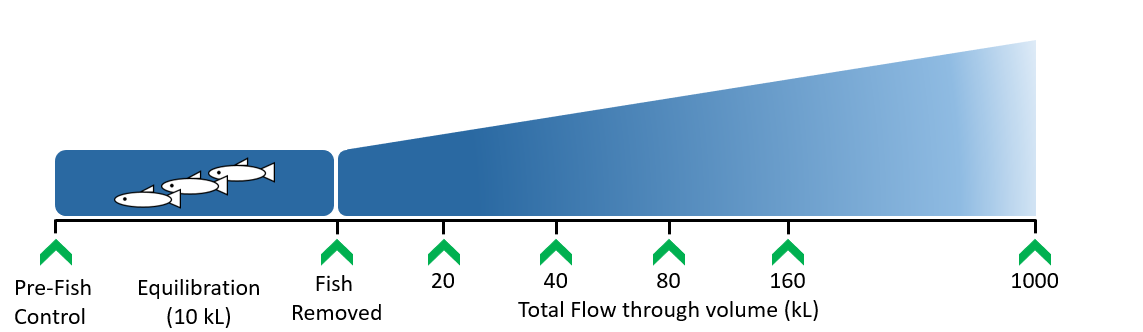
\includegraphics[scale=0.55,left]{Chapter4Images/dilutiontest.png}
\caption{ The Dilution Experiment \citep{fishforensics,hatchery}}
\label{fig:flowsamplinschedule1}
\end{figure}
		


Figure~\ref{fig:flowsamplinschedule1} depicts the dilution experiment. Three juvenile Coho salmon were placed in a minnow trap in each of four experimental tanks. The fish were left to equilibrate for nine days with flow through (140-155 L/minute). Traps containing the fish were then removed and accumulated eDNA was diluted via hatchery water flow-through. Pre-fish negative controls were collected for each tank, and fish-positive controls were collected after the nine-day equilibration period. Triplicate samples, indicated by the green arrows, at specified times representing aggregate flow-through volumes of 20, 40, 80, 160 and 1000 kL. Five negative control samples were taken concurrently from the hatchery pond (n = 3) and the hatchery kitchen sink (n= 2).

\vspace{5mm}

Each sample consisted of eight technical replicates, and each set of eight technical replicates was assigned a unique sort code. Technical replicates with sort codes equal to 31 and 84 did not pass integritE tests and were thus removed from the data set. These corresponded to samples from 20kL Flow, Tank 19 and from 1000kL Flow, Tank 20. There were an additional extra set of 12 sample replicates corresponding to 10kL Flow. These were stored in the excel file with special characters to indicate they were not to be included in analysis (because the samples had been taken after only three days, while the fish were still in the tanks opposed to after nine days). We include several tables summarizing how many samples were taken and the general method of the experiment.


\begin{table}[H]
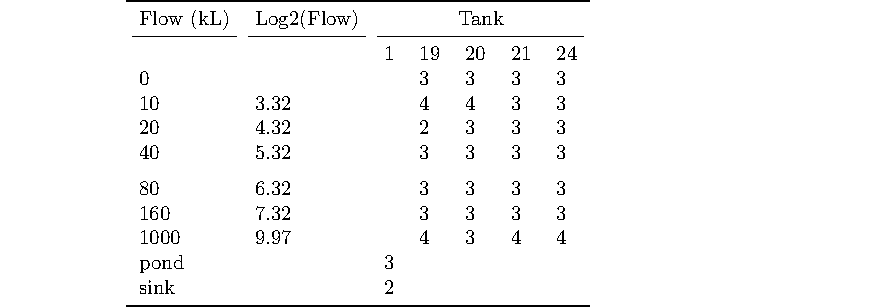
\includegraphics{Chapter4Images/flowkable1.pdf}
\caption{Summary of the number of sample replicates for each corresponding number of fish and Flow.}
\label{lab:flowkable1}
\end{table}

Table~\ref{lab:flowkable1} provides an overview summary of the samples taken for the dilution experiment. Also included is the number of sample replicates for sink and pond. Most levels of flow had three or four replicates taken from each tank. Two sample replicates were discarded since they did not appear to be valid measurements due to failure to pass DNA integritE tests. One was removed from tank 19 and 20kL flow and another was removed from tank 20 and 1000kL flow. The pond water had 3 sample replicates taken and the sink water had 2.
Note that for each sample replicate, there are eight associated technical replicates.



\begin{figure}[H]
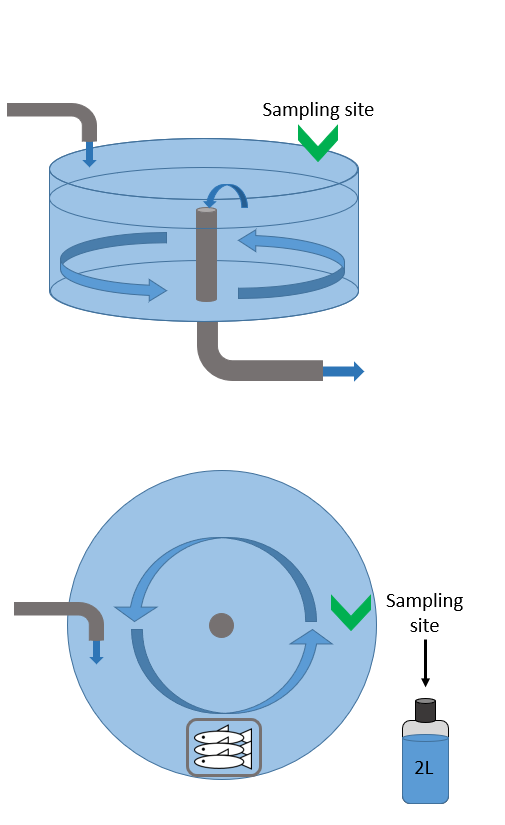
\includegraphics[scale=0.8]{Chapter4Images/flowsamplingroutinefixed.png}
\caption{Sampling routine for the flow experiment \citep{berg}.}
\label{fig:flowsamplingroutine}
\end{figure}

Figure~\ref{fig:flowsamplingroutine} represents the general method in which samples were taken. eDNA samples were taken from the opposite side of the inflow pipe. The tanks were all of size 1000kL. Three fish in a minnow trap were in each tank except for the pre-fish negative controls.



\vspace{5mm}

\begin{figure}[H]
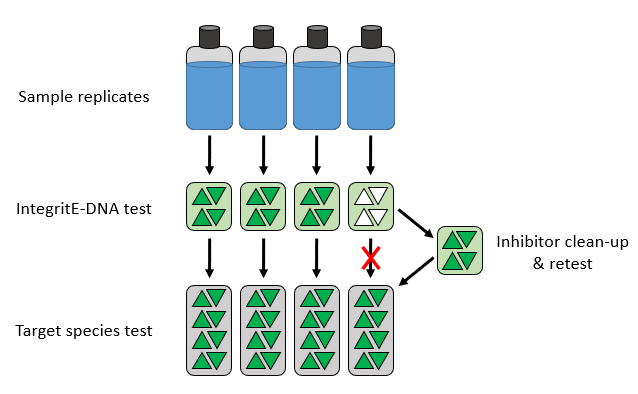
\includegraphics{Chapter4Images/flowprocedure.png}
\caption{Analysis procedure for the dilution experiment \citep{berg}.}
\label{fig:flowprocedure}
\end{figure}

Figure~\ref{fig:flowprocedure} represents the method in which quality of eDNA was assessed  before analysis. Sample replicates were first tested with integritE-DNA test. Samples which failed to pass integritE test were cleaned and retested before analysis.




\section{Flow Plots}



 First, we examine the `Pre-Fish Negative controls'. We plot the Sample.replicate number on the x-axis, and the transformed CT (TCT) of the associated eight technical replicates on the y-axis. These plots correspond to tanks which had just been filled by the infill pipe, and no additional water had been allowed to flow through the tank.


\begin{figure}[H]
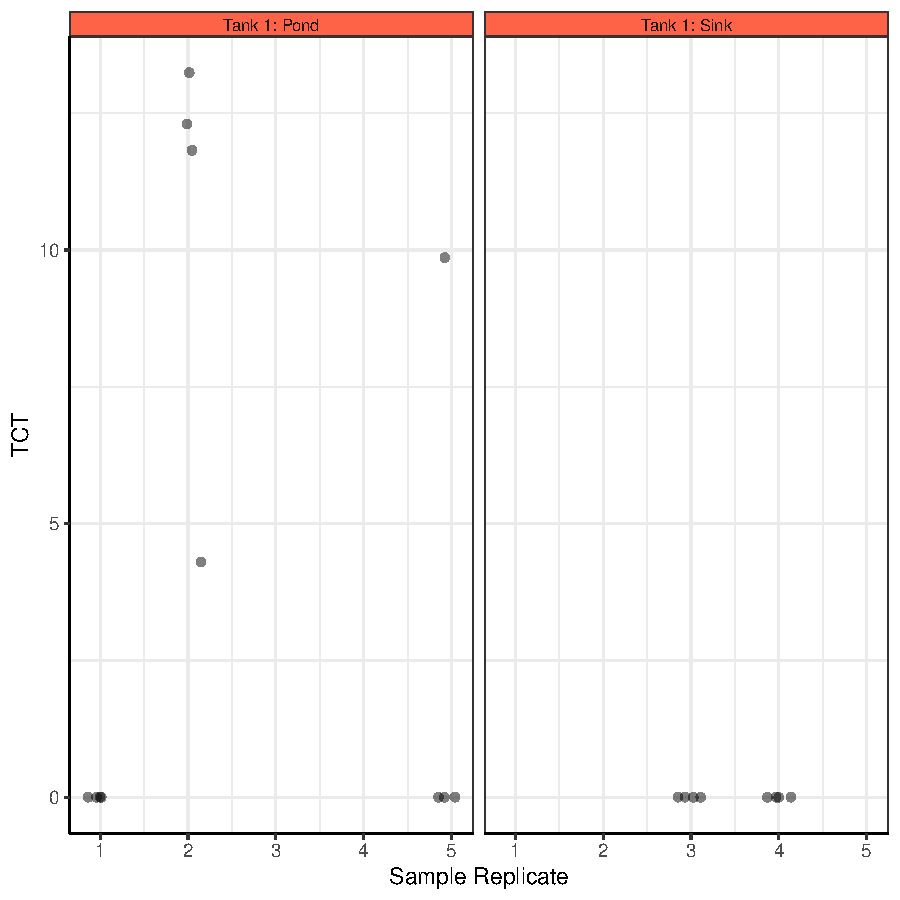
\includegraphics[scale=0.8]{Chapter4Images/pondandsink.pdf}
\caption{Transformed CT values obtained from samples taken from pond and sink water. Samples were taken from a small tank, tank 1.}
\label{fig:sinkandpond}
\end{figure}

Figure~\ref{fig:sinkandpond} are the plots of TCT values obtained from the hatchery sink and the hatchery pond. The water was transferred to tank 1 where sample replicates were then obtained. The goal of these measurements was to observe possible background hatchery signal of Coho eDNA. While the sink water showed no sign of Coho eDNA, the samples from the pond did indicate presence of Coho.




\begin{figure}[H]
\includegraphics[scale=0.8]{Chapter4Images/zerofishtct.pdf}
\caption{Transformed CT values obtained from pre-fish negative controls. }
\label{lab:flowzerofish}
\end{figure}

Figure~\ref{lab:flowzerofish} are the TCT plots obtained from the tanks before the fish were added. The samples help to measure a hatchery background signal of Coho eDNA. Most samples indicate no presence of Coho eDNA, although there exist several outliers. This may indicate that the hatchery water itself contains trace amounts of Coho eDNA.




\begin{figure}[H]
\includegraphics{Chapter4Images/finalflowplots.pdf}
\caption{Transformed CT values by sample replicate number obtained from samples taken from each tank at differing levels of dilution.}
\label{fig:finalflowplot}
\end{figure}





Figure~\ref{fig:finalflowplot} contains the TCT plots obtained from the tanks for the indicated levels of dilution. Note that the 10kL level corresponds to samples that were taken right after the fish were removed (prior to dilution). When only 20kL of water had been allowed to flow through the tank, we consistently detected eDNA. At 40kL of flow, we still had consistent detection, but the number of non-detects began to increase more significantly. By the time we reach 80kL, detection of Coho eDNA was no longer consistent. Presence of Coho eDNA was not being picked up, except in a small number of cases. For flows greater than 80kL, we are no longer consistently detecting Coho eDNA. However, there does exist the rare detection of Coho eDNA at even the higher levels of flow. This may be due to the background noise in the hatchery water that we previously discussed.


\section{Flow Models}
\subsection{Median Transformed CT}


We now fit statistical models for the response variable median TCT. Only data that was collected once the minnow trap was removed is included in this analysis. This corresponds to the six collection points in Figure 4.5. In general, as log2(Flow) increases, we would expect `CT' to rise and hence `TCT' to decrease as the shed eDNA was washed out of the tank. We first fit a simple linear model, flow.l.one.line. This model only considers log2(Flow) as a predictor.



\begin{figure}[H]
\includegraphics[scale=0.8]{Chapter4Images/flowmedtctgg.pdf}
\caption{Plot of Median TCT vs Log2(Flow) in kL, included is the simple linear model, flow.l.one.line and its associated 95\% confidence bands.}
\label{fig:flowmedtct}
\end{figure}


\begin{table}[H]
\includegraphics{Chapter4Images/flowloneline.pdf}
\caption{Parameter estimates and standard errors for a simple linear model on Median TCT. This model only considers log2(Flow) as a predictor. Model: flow.l.one.line. The $R^{2}$ for this model is 0.680.}
\label{fig:flow11}
\end{table}

Figure~\ref{fig:flowmedtct} is the plot of the regression line flow.l.one.line. Median Transformed CT is taken over each Sample.replicate vs Log2(Flow). Notice that at a certain point, median TCT approaches zero. That is, we no longer are detecting eDNA past a certain value of log2(Flow). We later use alternative models that account for this fact as it does not make sense to predict negative median TCT values. Table~\ref{fig:flow11} provides the estimates of the model flow.l.one.line. The estimated intercept is 24.46 with a standard error of 1.46 and the estimate for the flow term is -2.81. Both estimates have extremely small p-values, indicating high significance of both the intercept and slope. The $R^{2}$ is 0.68 which means our model does a reasonable job at explaining variation in the data. The $Pr(> |t|)$  is the p-value for the test of a zero parameter value. Since both the intercept and log2(flow) have small p-values, they should be included in the model.
 


\newpage

We now proceed as in Chapter 3, whereby we consider the impact of tank and interactions on the TCT values.  We fit a model flow.l.tank, that considers dilution as before and also considers the tank as a factor. This model thus allows the intercept to change depending on the tank; however, the slope for each tank remains constant. 

\vspace{5mm}


\begin{table}[H]
\includegraphics{Chapter4Images/flowltank.pdf}
\caption{Parameter estimates and standard errors for a linear model on Median TCT. This model allows for differing intercepts among tanks. Model: flow.l.tank.  The $R^{2}$ for this model is 0.689.}
\label{fig:flow12}
\end{table}

Table~\ref{fig:flow12} is a summary of our model that  includes the tank number as a factor.  As before, there is a high level of significance for the intercept and flow terms. Each tank has an associated coefficient term. The baseline tank is tank 19. For example, a sample corresponding to Tank 20 would have an intercept of 23.25+1.73 and a slope of -2.79. The individual p-values for each tank do not immediately appear significant. However, this does not guarantee that tank itself is not important. To conclude that, we would need to compare this model with a model that does not contain tanks, we can do this using `anova'.  The $R^{2}$ for flow.l.tank 0.689, which is only slightly larger than the $R^{2}$ for flow.l.one.line. Moreover, the adjusted $R^{2}$ which accounts for number of predictors is now actually less than the $R^{2}$ of flow.l.one.line.

\newpage

We also fit a  model flow.l.four.line that considers flow, tank as a factor and also the interaction between tank and biomass. This will allow not only for differing intercepts, but also differing slopes for each tank.

\vspace{5mm}

\begin{table}[H]
\includegraphics{Chapter4Images/lfourlinemed.pdf}
\caption{Parameter estimates and standard errors for a model that includes tank and the interaction between tank and log2(flow). Intercepts and slopes are allowed to differ for each tank. Model: flow.l.four.line. The $R^{2}$ for this model is 0.692.}
\label{fig:flow13}
\end{table}

Table~\ref{fig:flow13} summarizes the model flow.l.four.line. This model includes tank and the interaction between tank and log2(Flow). The output indicates that neither tank, nor the interaction are significant. The interaction terms are multiplications of flow and the tank indicator terms. These terms would cause a different slope depending on which tank the sample was taken.

\newpage

 We now preform an `anova (extra sum of squares)' test to see which of our models is significant; 
\vspace{5mm}

\begin{table}[H]
\includegraphics{Chapter4Images/anovamed.pdf}
\caption{Extra sum of squares test results for  the three flow models on median TCT.}
\label{fig:anovaflow}
\end{table}


  
  
Table~\ref{fig:anovaflow} provides the results of the extra sum of squares test. The full model,  flow.l.four.line allows both the intercept and slopes to differ depending on which tank the sample is taken from.
We compare this model with the model flow.l.tank to test for the hypothesis of differing slopes between tanks. Because the p-value is large (p=0.87) , we cannot reject the hypothesis that the coefficient for additional slopes is zero. Similarly, when comparing flow.l.tank with flow.l.one.line, the hypothesis is that the coefficient that determines differing intercepts among tanks is zero. Because the p-value is again large (p=0.586), we cannot reject (at the 0.05 significance level) the hypothesis that the coefficient is zero. Hence, we conclude that both tank and the interaction between tank and Log2(Flow) are not needed in our models.










\subsection{Flow Models (Mean)}

We now fit statistical models for the response variable mean TCT. First, we fit a simple linear model, flow.l.one.line.mean. This model only considers log2(Flow) as a predictor.

\vspace{5mm}


\begin{table}[H]
\includegraphics{Chapter4Images/flowlonelinemean.pdf}
\caption{Parameter estimates and standard errors for simple linear model for Mean TCT which only considers log2(Flow) as a predictor. Model: flow.l.one.line.mean. The $R^{2}$ for this model is 0.692.}
\label{fig:meanflow1}
\end{table}

Table~\ref{fig:meanflow1} summarizes flow.l.one.line.mean. The output provides estimates of an intercept of 23.85 and a slope term on log2(Flow) of -2.69. The $ R^{2}$ is 0.692 and the adjusted $R^{2}$ is 0.688.
 

\newpage

We now fit a model, flow.l.tank.mean that also includes the tank number as a factor.  As before, R indicates high significance for the intercept and flow terms.

\vspace{5mm}

\begin{table}[H]
\includegraphics{Chapter4Images/flowltankmean.pdf}
\caption{Parameter estimates and standard errors for a model on Mean TCT that considers tank as a predictor in addition to log2(Flow). Model: flow.l.tank.mean. The $R^{2}$ for this model is 0.699.}
\label{fig:meanflow2}
\end{table}

Table~\ref{fig:meanflow2} summarizes the model flow.l.tank.mean. The estimated intercept for tank 19  is 22.82 and the slope coefficient is -2.68. The $R^{2}$ for the new mean model is 0.699 , however the adjusted $R^{2}$ has now decreased to 0.682. The individual p-values for each tank do not immediately  appear significant. However, this does not guarantee that tank itself is not important. To conclude that, we need to compare this model with a model that does not contain tanks, we can do this using `anova'.
  


\begin{table}[H]
\includegraphics{Chapter4Images/lfourlinemean.pdf}
\caption{Parameter estimates and standard errors for a model on Mean TCT that includes log2(Flow), Tank, and the interaction between log2(Flow) and Tank. Model: flow.l.four.line.mean. The $R^{2}$ for this model is 0.702.}
\label{fig:meanflow3}
\end{table}

 This model includes tank and the interaction between tank and log2(Flow). Hence this allows for both intercepts and slopes to differ between each tank. The results indicate that neither tank, nor the interaction terms are significant. 

\vspace{5mm}


\begin{table}[H]
\includegraphics{Chapter4Images/anovameanF.pdf}
\caption{ANOVA table for flow models.}
\label{fig:anovaflow1}
\end{table}


 Table~\ref{fig:anovaflow1} shows the results of the `anova (extra sum of squares)' test to see which of our models for mean TCT is significant. We first consider the full model  flow.l.four.line.mean that allows for different slopes and different intercepts. Comparing flow.l.four.l.mean with flow.l.tank.mean is a test of equality of slopes. Since the p-value is large, we cannot reject the null hypothesis that the terms are identical. That is, we cannot reject the hypothesis that the slopes do not differ among tanks. Next we compare flow.l.tank.mean with flow.l.one.line.mean, which is a test of differing intercepts. Similarly, we obtain a large p-value (p=0.68) and hence cannot reject the hypothesis that the intercepts do not differ. Thus, as before, we conclude that working with a model that only includes log2(flow) as a predictor is sufficient.

















\section{Alternative Models}



As seen above, once the dilution is large enough, we no longer detect the presence of Coho eDNA. Hence our statistical model should account for this asymptotic property. We fit and compare a variety of  non-linear models. These include the `broken stick' model for mean TCT, hyperbolic tangent models, Lowess models and finally a `Bent Cable Model' \citep{piecewiseregression}. In this analysis we include models fit to the response variable Mean Transformed CT. The models for median Transformed CT are very similar.

\subsection{Broken Stick Models}

Firstly, we fit what is known as a broken stick model. The broken stick model is a non-linear regression model that allows for sharp changes in direction.
The model includes a `break point', $\gamma$, that is used to fit a model. We use the R function `nls' \citep{nlsTools} which stands for `Nonlinear Least Squares' to fit the model. This function allows us to obtain `weighted' estimates of the parameters.

\vspace{3mm}

The Broken Stick model has the form:

\vspace{3mm}

 $$ \beta_{0}+\beta_{1}x+ \begin{cases}
0  &  \text{if    } x \le \gamma \\[2ex]
\beta_{2}(x-\gamma)  & \text{if    } x > \gamma
\end{cases}$$


This can be written as:

$$\beta_{0}+\beta_{1}x \hspace{1mm} \mbox{ for} \hspace{2mm} x \le \gamma \hspace{1mm} \mbox{, and}$$


$$\beta_{0}+\beta_{1}x+\beta_{2}(x-\gamma)=(\beta_{0}-\beta_{2}\gamma)+(\beta_{1}+\beta_{2})x \hspace{2mm} \mbox{for} \hspace{2mm}  x > \gamma \mbox{.} $$.


\begin{figure}[H]
\includegraphics[scale=0.7]{Chapter4Images/meanbrokenstick.png}
\caption{Broken Stick model for Mean TCT (top) and the associated residuals for the model (bottom).}
\label{fig:brokenstickmean}
\end{figure}

%\begin{figure}[H]
%\includegraphics[scale=0.7]{tablesandimages/brokenstickmean1.pdf}
%\caption{Broken-Stick model for Mean Transformed CT and the associated residuals for the model }
%\label{fig:brokenstickmean}
%\end{figure}


Figure~\ref{fig:brokenstickmean} shows the broken stick regression line in red. The `breakpoint', $\gamma$ is estimate 6.877 (s.e 0.266). The estimate for $\beta_{0}$ is 33.374 (s.e 1.74), $\beta_{1}$ has an estimate of -4.931 (s.e 0.347) and $\beta_{2}$ is estimated to be 4.932 (s.e 0.555). Also included is the residual plot for the Broken-stick model. The fitted values are the predicted mean TCT for a given log2(Flow) value. On the y-axis are the actual residuals, the difference between the true value and the fitted value. The `RSS' (Residual Sum of Squares) for this model is 614.761.



\subsection{Bent Cable Models}


 In the previous analysis we fit broken stick models. We can see that in the broken stick models, the break point causes a sharp turn. However, it may be more reasonable and biologically sound to fit a more flexible model. Hence, we make use of the ``bent cable" model that allows for a smoother model \citep{bentcable}. We use the bentcable function \citep{bentcable2}.
 
 \vspace{5mm}
 
The Bent Cable model takes the form:
\vspace{5mm}


 $$ \beta_{0}+\beta_{1}x+ \begin{cases}
0  &  \text{if    } x < \alpha-\gamma \\[2ex]
\beta_{2}\frac{(x-\alpha+\gamma)^{2}}{4\gamma}  &  \text{if    } \alpha-\gamma  \le x \le \alpha+\gamma \\[2ex]
\beta_{2}(x-\alpha) & \text{if  } x > \alpha+\gamma
\end{cases}$$



\begin{figure}[H]
\includegraphics[scale=0.7]{Chapter4Images/meantctbentcable.png}
\caption{Bent Cable Model for Mean TCT (top) and the associated residuals for the model (bottom).}
\label{fig:meanbc}
\end{figure}





Figure~\ref{fig:meanbc}  is the plot of the bent cable model and the associated residual plot. The red line is the bent cable regression line. The $\alpha$ value is estimated as 6.89 (s.e 0.542), the $\gamma$ value is estimated 0.565 (s.e 0.124) and the log-likelihood  is -189.24. The estimate for $\beta_{0}$ is 34.350 (s.e 1.51), $\beta_{1}$ has an estimate of -4.925 (s.e 0.288) and $\beta_{2}$ is estimated to be 4.940 (s.e 0.550). The parameter $\alpha$ is the breakpoint discussed above, while $\gamma$ is a parameter that impacts the length of the quadratic portion connecting the two linear sections of the regression line. The RSS for this model is 614.767. 

\newpage

\subsection{Hyperbolic Tangent Models}

We can also fit models similar to `bent cables' that utilize the hyperbolic tangent function to allow for smoothness.

\vspace{12pt}
 
The tanh model takes the form:

$$\beta_{0}+\beta_{1}(x-\alpha)+\beta_{2}(x-\alpha)\tanh(\frac{x-\alpha}{\gamma})$$

where $\tanh(z)=\frac{e^{z}-e^{-z}}{e^{z}+e^{-z}}$ is the hyperbolic tangent function.



\begin{figure}[H]
\includegraphics[scale=0.7]{Chapter4Images/tanhmodel.png}
\caption{Hyperbolic Tangent (tanh) model for Mean TCT (top) and the associated residuals for the model (bottom).}
\label{fig:meantanh}
\end{figure}


Figure ~\ref{fig:meantanh} is the tanh model and residuals for mean TCT. The purple line is the tanh regression line. For mean TCT, our hyperbolic tangent model estimates the break point `br' ($\alpha$) to be $\alpha=6.887$ (s.e 0.448). R estimates $\gamma= -0.776$ (s.e 4.82) , $\beta_{0}=0.8920$ (s.e 2.80), $\beta_{1}=-2.46$ (s.e 0.350) and $\beta_{2}=-2.33$ (s.e 1.03). The residuals look good as they appear to be randomly distributed about the y-axis. The RSS for the tanh model is 595.239.


\subsection{Lowess Models}

We fit similar models using the `lowess' function in R. lowess stands for locally-weighted polynomial regression.
 The lowess models are quite `sharp'. They both appear similar to our `broken stick' models. We used a smoothing parameter value of 3/4 and allowed the algorithm to perform three iterations.



\begin{figure}[H]
\includegraphics[scale=0.7]{Chapter4Images/meantctlowess.png}
\caption{Lowess model for Mean TCT (top) and the associated residuals for the model (bottom).}
\label{fig:meanlowess}
\end{figure}


Figure~\ref{fig:meanlowess} shows the lowess model for mean TCT and the associated residuals. The purple line represents the line of best fit according to the lowess criteria. This model looks very similar to the broken-stick model. This model estimates an intercept of 24.42 (s.e 0.894) and a lowess parameter of -2.74 (s.e 0.136). The residuals look good as they appear to be randomly distributed about the y-axis. The RSS for the lowess model is 589.698.




\newpage

\subsection{Model Comparison}

\begin{figure}[H]
\includegraphics[scale=0.9]{Chapter4Images/meanTCTmodelcomparison.pdf}
\caption{Model comparison for four distinct models for the response variable mean TCT. Here we plot a broken-stick model, a lowess model, a hyperbolic tangent model and a bent-cable model.}
\label{fig:modelcomparison}
\end{figure}

Figure~\ref{fig:modelcomparison} plots all of our non-linear models for mean TCT. They all appear to be quite similar to one another. The broken-stick model appears to have a very sharp turn at the breakpoint, while the bent cable makes a more smooth transition.  The log-likelihood for the broken stick model is -189.24, which is the same as the log-likelihood for the bent-cable model. The log-likelihood for the Lowess and Tanh models is -185.34 and -187.99 respectively.


\begin{table}[H]
\includegraphics{Chapter4Images/nichealternate.pdf}
\caption{Model comparison for four distinct models for the response variable mean TCT. Here we plot a broken-stick model, a lowess model, a hyperbolic tangent model and a bent-cable model.}
\label{lab:comtable}
\end{table}


Table~\ref{lab:comtable} is a summary of our non-linear models. All four of the models are quite similar, and while the RSS for the bent-cable is slightly higher than that of the Lowess, we still chose to work with the Bent Cable due to the biological interpretation and smooth break point.


\newpage

The final model that we choose is the bent cable model. We choose this because it has a low log-likelihood and also makes biological sense. The bend represents the point of time in which eDNA is no longer detectable due to dilution. The RSS of the bent cable model is also not much larger than the RSS of the other three models.



\begin{figure}[H]
\includegraphics{Chapter4Images/flowggplot1.pdf}
\caption{ A bent cable model for mean TCT.}
\label{fig:bentcablemean}
\end{figure}


Figure~\ref{fig:bentcablemean} is a plot of our bent-cable model. The $\alpha$ value (estimated breakpoint) is 6.89 and is represented by the solid vertical line, the $\gamma$ value is 0.565 and the log-likelihood is -189.24. Included are the confidence regions for the regression line. Also included is the confidence interval for the breakpoint represented by the vertical dashed lines. The $\gamma$ value is a parameter that controls the length of the quadratic portion of the curve.
\section{Dilution Conclusions}

The Dilution experiment allowed us to study the impact of flow on the collection of Coho eDNA samples. This study provided a  controlled environment to study the loss of eDNA signal via degradation  after the Coho had been removed from the tanks. The collection of plots organized in Table~\ref{fig:finalflowplot} illustrate the general trend. At the time of fish removal, TCT values were highest and sample replicates frequently had mean TCT values exceeding 15.  As seen in Figure~\ref{fig:finalflowplot}, at dilution levels of 160 kL and 1000 kL, TCT levels were not significantly different than background hatchery signals (Table~\ref{lab:flowzerofish}).

\vspace{5mm}

In the dilution experiment, Coho eDNA was detected at the 20kL dilution with 100\% reliability at the technical replicate level. At the 40kL level of dilution, Coho eDNA was detected in all but two sample replicates. Technical replicate non-detections occurred in eight of twelve sample. At 80kL dilution, only one sample replicate level detection was made, with 4 out of 8 qPCR replicates successfully amplifying target DNA. For dilutions greater than 80kL, we were not able to confirm presence with perfect detection, although several of the samples had 1 to 2 of 8 technical replicate detections.

\vspace{5mm}

We first fit several linear models, summarized in Table~\ref{lab:flowsum}.

\begin{table}[H]
\includegraphics{Chapter4Images/flowsummary.pdf}
\caption{Table of comparison for the linear models fitted. Due to the breakpoint, we decided to leave linear models behind and work with non-linear models.}
\label{lab:flowsum}
\end{table}

\vspace{5mm}

Because there appeared to be a point at which the impact of dilution made Coho eDNA measurement negligible, we used a non-linear, bent cable model to fit a model for mean TCT. This model accounted for a  `break-point'. As seen in Figure~\ref{fig:bentcablemean}. Our breakpoint of $\log2(x)=6.89$ would represent a dilution of 118 kL. This could be thought of as the point at which Coho eDNA collection is no longer differentiable from the hatchery background signal. The confidence region for the breakpoint was computed by using the standard error of the model. The 95 \% confidence interval for the breakpoint ranged from 5.83 to 7.96 on the log2 scale. These points cover the range of dilutions from 56.96 kL to 247.28 kL. 



\startchapter{Field Data}
\label{chapter:Fieldalt}


While Chapter 3 and Chapter 4 analyzed controlled experiments, one goal of eDNA technology is its usage in the field. To study how eDNA analysis can be used to detect Coho Salmon in the wild, several field studies were conducted. In particular, four streams in British Columbia were studied (steams AAA, BBB, CCC and DDD). Water samples were collected and associated environmental and physical covariates were recorded. The main fish species of interest was Coho Salmon (\textit{Oncorhynchus kisutch}), although we also considered Cutthroat Trout (\textit{Oncorhynchus clarkii}) and Rainbow Trout (\textit{Oncorhynchus mykiss}). Ecofish personnel also took biomass measurements of each of the species caught using electrofishing.  All biomass measurements were obtained using electrofishing, a method that involves using electric current to temporarily shock and stun fish. Researchers recorded the weight of Coho Salmon, Cutthroat Trout and Rainbow Trout and also recorded the overall weight of all fish that were caught.

\vspace{4mm}

The dataset consists of 432 observations. From each of the four streams, distinct sample locations were chosen. For each sample location, sample replicates were taken each of which consisted of eight observations or technical replicates. Hence there were  432/8= 54 sample replicates as each sample replicate consisted of 8 technical replicates. Nine sample replicates were from stream AAA, nine sample replicates were from stream BBB, eighteen of the sample replicates were from stream CCC and the remaining eighteen sample replicates were from stream DDD. The reason eighteen samples were collected from stream CCC and stream DDD is because two distinct reaches in these streams were studied. Nine replicates were chosen from each reach within these two streams. Samples were collected from streams AAA, BBB and DDD in 2017, while samples from stream CCC were collected in 2018. Within each stream, multiple distinct sections of the stream were chosen to take samples from. These distinct sections are referred to in the dataset as sites.

\vspace{5mm}

In this data analysis we considered the possible impact of covariates on TCT measurements. Firstly, we include the total biomass for each species that was caught in the transect (CO.Total.Biomass.g for Coho). We also included the total biomass per meter squared of transect (CO.Biomass.g.m2 for Coho) and total biomass per meter cubed of transect (CO.Biomass.g.m3 for Coho) calculated using the dimensions of the transect. The environmental covariates that we included were water temperature (Water.Temperature.C), pH, flow rate (Transect.Flow.cms), the distance from shore in meters from which the eDNA sample was taken (eDNA.Distance.from.Shore.m) and the depth of water in meters from which the sample was taken (eDNA.Total.Water.Depth.m). Moreover, we included the possibility of interactions between flow rate and all biomass variables.

\vspace{5mm}

We attempt to show that by accounting for common covariates, researchers may save time and obtain comparable estimates of biomass/abundance to those obtained using costly standard sampling methods such as electrofishing.  We highlight the need for continued research into this topic. Results for Rainbow Trout and Cutthroat Trout can be found in the Appendix. In the following pages, we include summary plots for each of the four streams. We include the total biomass of all fish and Coho Salmon caught in each stream and their associated TCT scores for each sample replicate.


\newpage

\section{Streams}

\subsection{Stream AAA}


\begin{figure}[H]
\centering
\includegraphics{Chapter5Images/AAA_Ef_new.pdf}
\caption{ Total Biomass for all fish at stream AAA.}
\label{fig:AAA_ef}
\end{figure}



\begin{figure}[H]
\centering
\includegraphics{Chapter5Images/AAA_ef_tct.pdf}
\caption{ Transformed CT values of the technical replicates for all fish at stream AAA.}
\label{fig:AAA_ef2}
\end{figure}






\begin{figure}[H]
\centering
\includegraphics{Chapter5Images/AAA_Co_new.pdf}
\caption{  Total Biomass for Coho Salmon at stream AAA.}
\label{fig:AAA_coho}
\end{figure}



\begin{figure}[H]
\centering
\includegraphics{Chapter5Images/AAA_co_tct.pdf}
\caption{  Transformed CT values of the technical replicates for Coho Salmon.}
\label{fig:AAA_co}
\end{figure}


Figure~\ref{fig:AAA_ef} is a plot of the total biomass for all fish species collected from the three sites at stream AAA. At each site, fish were caught in the transects. Figure~\ref{fig:AAA_ef2} is a plot of the associated TCT values obtained from each site using a primer that amplifies all fish.
\vspace{5mm}
Figure~\ref{fig:AAA_coho} shows that no Coho Salmon were caught at stream AAA. Although Figure~\ref{fig:AAA_co} indicates that there was trace detection of Coho at each of the three sites.


\newpage

\subsection{Stream BBB}



\begin{figure}[H]
\centering
\includegraphics{Chapter5Images/BBB_Ef_new.pdf}
\caption{ Total biomass of all fish at each site for stream BBB.}
\label{fig:testBBBbiom}
\end{figure}



\begin{figure}[H]
\centering
\includegraphics{Chapter5Images/BBB_ef_tct.pdf}
\caption{ Transformed CT values of the technical replicates for all fish.}
\label{fig:BBB_ef}
\end{figure}




\begin{figure}[H]
\centering
\includegraphics{Chapter5Images/BBB_Co_new.pdf}
\caption{ Total biomass for Coho Salmon at each site for stream BBB.}
\label{fig:testBBBbiomCo}
\end{figure}




\begin{figure}[H]
\centering
\includegraphics{Chapter5Images/BBB_co_tct.pdf}
\caption{ Transformed CT values of the technical replicates for Coho Salmon.}
\label{fig:BBB_co}
\end{figure}

Figure~\ref{fig:testBBBbiom} is a plot of the total biomass for all fish species collected from the three sites at stream BBB. At each site, fish were caught in the transects. Site number 1 had the highest recorded biomass, although each site had less biomass than those caught in stream AAA. 

\vspace{5mm}

Figure~\ref{fig:BBB_ef} is a plot of the associated TCT values obtained from each site at stream BBB using a primer that amplifies all fish. We see that each site detected relatively high TCT values indicating the presence of fish.

\vspace{5mm}

Figure~\ref{fig:testBBBbiomCo} is a plot of the Coho Salmon that were caught at stream BBB. At each site in stream BBB, Coho were caught. Figure~\ref{fig:BBB_co} confirms the presence of Coho by the moderate TCT values. 

\newpage

\subsection{Stream CCC}




\begin{figure}[H]
\centering
\includegraphics{Chapter5Images/CCC_Ef_new.pdf}
\caption{ Total biomass of all fish at each site for stream CCC.}
\label{fig:testCCCbiomEf}
\end{figure}



\begin{figure}[H]
\centering
\includegraphics{Chapter5Images/CCC_ef_tct.pdf}
\caption{ \hspace{1mm} Transformed CT values of the technical replicates for all fish.}
\label{fig:CCC_ef}
\end{figure}



\begin{figure}[H]
\centering
\includegraphics{Chapter5Images/CCC_Co_new.pdf}
\caption{  \hspace{1mm}Total biomass for Coho Salmon at each site for stream CCC.}
\label{fig:testCCCbiomCo}
\end{figure}





\begin{figure}[H]
\centering
\includegraphics{Chapter5Images/CCC_co_tct.pdf}
\caption{  \hspace{1mm}Transformed CT values of the technical replicates for Coho Salmon.}
\label{fig:CCC_co}
\end{figure}

Stream CCC had two distinct sections, a diversion and a upstream portion. Measurements were thus taken from three distinct sites in each of these distinct portions. Figure~\ref{fig:testCCCbiomEf} shows the biomass of all fish caught at stream CCC. Figure~\ref{fig:CCC_ef} shows the associated TCT values that were obtained from the collected samples.
We see from Figure~\ref{fig:testCCCbiomCo} that no Coho were caught at any portion of this stream. Moreover, Figure~\ref{fig:CCC_co} had no detection of any Coho in any sample.

\newpage

\subsection{Stream DDD}



\begin{figure}[H]
\centering
\includegraphics{Chapter5Images/DDD_Ef_new.pdf}
\caption{  \hspace{1mm}Total biomass for all fish at each site for stream DDD.}
\label{fig:testDDDef}
\end{figure}



\begin{figure}[H]
\centering
\includegraphics{Chapter5Images/DDD_ef_tct.pdf}
\caption{  \hspace{1mm}Transformed CT values of the technical replicates for all fish.}
\label{fig:DDD_ef}
\end{figure}

\begin{figure}[H]
\centering
\includegraphics{Chapter5Images/DDD_Co_new.pdf}
\caption{  \hspace{1mm}Total biomass for Coho Salmon at each site for stream DDD.}
\label{fig:testDDDco}
\end{figure}





\begin{figure}[H]
\centering
\includegraphics{Chapter5Images/DDD_co_tct.pdf}
\caption{ \hspace{1mm} Transformed CT values of the technical replicates for Coho Salmon.}
\label{fig:DDD_co}
\end{figure}


Stream DDD had two distinct sections, a diversion and a downstream portion. Measurements were thus taken from three distinct sites in each of these distinct portions.
Figure~\ref{fig:testDDDef} shows the biomass of all fish caught at stream DDD. Figure~\ref{fig:DDD_ef} shows the associated TCT values that were obtained from the collected samples.
We see from Figure~\ref{fig:testDDDco} that no Coho were caught at any portion of this stream. However, Figure~\ref{fig:DDD_co} indicates trace detection of Coho Salmon at both the diversion and downstream.



\section{Pairs Plots}



	We now examine how several covariates are associated with one another. We visualize these possible relationships using a `pairs plot'. These plots help illustrate how several variables are possibly correlated. We consider the density and flow terms, as well as previously identified important environmental covariates.  In the case of all fish, one outlier was removed after failing to pass the DNA integrit-E test (this observation was from stream DDD, diversion). The outlier can be seen in the first pairs plot as a blue dot in the bottom left of the first image, in the portion comparing Fish.Total.Biomass.g with MeanTCTEf. The pairs plot compares each predictor with one-another. For example, the first row contains a scatter plot of mean TCT versus each of the other covariates.



\begin{figure}[H]
\includegraphics{Chapter5Images/EFishpairs_outlierincluded.pdf}
\caption{  \hspace{1mm}  Pairs plots for all fish with outlier included. We consider several suspected key covariates. Black corresponds to stream AAA, red corresponds to stream BBB, green corresponds to stream CCC and blue corresponds to stream DDD.}
\label{fig:pairefoi}
\end{figure}




\begin{figure}[H]
\includegraphics{Chapter5Images/EFishpairs.pdf}
\caption{  \hspace{1mm}  Pairs plots for all fish with outlier removed. We consider several suspected key covariates. Black corresponds to stream AAA, red corresponds to stream BBB, green corresponds to stream CCC and blue corresponds to stream DDD.}
\label{fig:pairef}
\end{figure}


\begin{figure}[H]
\includegraphics{Chapter5Images/Cohopairs.pdf}
\caption{  \hspace{1mm}Pairs plots for Coho Salmon. Black corresponds to stream AAA, red corresponds to stream BBB, green corresponds to stream CCC and blue corresponds to stream DDD.}
\label{fig:pairco}
\end{figure}

\newpage

The Pairs Plots confirm several of our assumptions. MeanTCT tends to increase linearly as biomass increases. MeanTCT also tends to decrease linearly as Transect.Flow.cms increases. Figure~\ref{fig:pairefoi} is the pairs plot for all fish in which the outlier was included. Figure~\ref{fig:pairef} is the same pairs plot but the outlier from stream DDD diversion was removed. Not much can be analyzed from these plots as there does not appear to be any obvious patterns. However, we see from the colors that samples from the same stream tend to cluster together. Figure~\ref{fig:pairco} is the pairs plot for Coho. We see from observing the first row that MeanTCT appears to increase linearly with CO.Total.Biomass.g, CO.Biomass.g.m2 and CO.Biomass.g.m3. MeanTCT also appears to possibly increase with higher water temperatures (Water.Temperature.C), and possibly decreases with higher levels of pH. MeanTCT also appears to decrease as Transect.Flow.cms increases.



\newpage

\section{TCT versus Biomass}

Although several covariates likely influence mean transformed CT scores, we expect a relationship between biomass and TCT. We visualize this one variable (mean over eight technical replicates) using a simple linear regression model before the addition of covariates.


Firstly, we considered linear models with biomass as the only predictor for Mean TCT.  Biomass refers to the weight in grams of the fish caught in the transect using electrofishing. 

\vspace{3mm}



\begin{figure}[H]
\includegraphics{Chapter5Images/gg_ef.pdf}
\caption{ \hspace{1mm} Mean TCT over each set of eight technical replicates versus Total Biomass for All Fish, outlier removed. Included is the simple linear regression model and the 95\% Confidence limits for the regression line.}
\label{fig:efanalysis}
\end{figure}


\begin{table}[H]
\includegraphics{Chapter5Images/eflinearfield.pdf}
\caption{Parameter estimates and standard errors for a model that considers biomass for all fish. Model: model.fish.}
\label{fig:modelef}
\end{table}


 Figure~\ref{fig:efanalysis} is the plot of the model, model.fish and the associated confidence limits. The line appears flat, and no obvious relationship is clear from a simple visual consideration. Table~\ref{fig:modelef} provides a summary of the simple linear model (model.fish) fit for All Fish. The $R^{2}$ is only 0.00093. Although the estimate for the coefficient of biomass is still positive, the estimate is not statistically significant. 


\begin{figure}[H]
\includegraphics{Chapter5Images/model_CO.pdf}
\caption{  \hspace{1mm}Mean TCT over each set of eight technical replicates versus Total Biomass for Coho Salmon. Included is the simple linear regression model (Biomass as the only predictor) and the 95\% Confidence limits for the regression line.}
\label{fig:cohoanalysis}
\end{figure}


\begin{table}[H]
\includegraphics{Chapter5Images/coholinearfield.pdf}
\caption{Parameter estimates and standard errors for a simple linear model for Coho. Model: model.co.}
\label{fig:modelco}
\end{table}



For Coho Salmon, our estimated positive of coefficient of +0.26 on biomass is statistically significant.  Figure~\ref{fig:cohoanalysis} makes the relationship clear. Mean TCT increases as CO.Total.Biomass.g increases. Table~\ref{fig:modelco} provides the summary of the simple linear model for mean TCT for Coho. The simple linear model only considered the predictor CO.Total.Biomass.g and achieved an $R^{2}$ of 0.600



\subsection{Environmental Factors}


We now consider the possible impact of covariates on the Mean TCT value. We include summary statistics of several of those covariates that have been shown to impact eDNA degradation such as pH and water temperature. We also include several biomass related terms such as total biomass, total biomass per meter squared of transect and total biomass per meter cubed of transect. We also include a `flow' term by considering the flow through the transect. 



\begin{table}[H]
\includegraphics{Chapter5Images/biomass_kable.pdf}
\caption{ \hspace{1mm} Table showing the total biomass (g) of each species captured in the transect for each site.}
\label{fig:kablemass}
\end{table}


Table~\ref{fig:kablemass} summarizes the total biomass of Coho, Cutthroat, Rainbow and all Fish that were caught in the transects in each site at each stream. Coho was only caught in stream BBB.


\begin{table}[H]
\includegraphics{Chapter5Images/kable_gm2.pdf}
\caption{   \hspace{1mm}Table showing the total biomass (g) of each species captured in the transect per meter squared of transects for each site.}
\label{fig:kablemass2}
\end{table}



\begin{table}[H]
\includegraphics{Chapter5Images/kable_gm3.pdf}
\caption{  \hspace{1mm} Table showing the total biomass (g) of each species captured in the transect per meter cubed of transects for each site.}
\label{fig:kablemass3}
\end{table}



%\begin{table}[H]
%\includegraphics{tablesandimages/kable_full.pdf}
%\caption{  \hspace{1mm}  Table showing a variety of summary statistics taken over each site. Temperature is in Celsius, pH is a scale and Transect Flow is in (cm/s).}
%\label{fig:kabletemp}
%\end{table}



\begin{table}[H]
\includegraphics{Chapter5Images/test_update.pdf}
\caption{  \hspace{1mm}  Table showing a variety of summary statistics taken over each site. Temperature is in Celsius, pH is a scale and Transect Flow is in (cm/s), Depth is the depth of the sample area in meters, and Distance is the distance in meters from shore in which the sample was taken.}
\label{fig:kabletemp}
\end{table}

Table~\ref{fig:kablemass2} summarizes the weight of each species caught per meter squared of transect. Table~\ref{fig:kablemass3} shows the weight of each species caught per volume of transect, calculated by using the depth of the transect. The reason that the weight per volume is larger than the weight per area is due to the fact that the transect depth was often very shallow and less than 1 meter. Table~\ref{fig:kabletemp} summarizes a variety of covariates that were recorded at each stream. These environmental covariates are taken into account in our statistical models. 


\newpage

\subsection{Models with Covariates}

To determine a suitable model for mean TCT for Coho we used backward elimination. Other than biomass per meter cubed of transect (CO.Biomass.g.m3), the original covariates that we considered were the water temperature in Celsius (Water.Temperature.C), the pH, the flow rate (Transect.Flow.cms), and the interaction between Transect.Flow.cms and CO.Biomass.g.m3. We also considered sampling covariates such as the sampling depth (eDNA.Water.Sampling.Depth.cm) and the distance from shore in which the sample was collected (eDNA.Distance.from.Shore.m).

\vspace{5mm}

The initial `full' model is named model.coho.full;

\vspace{5mm}

\begin{table}[H]
\includegraphics{Chapter5Images/cohofull.pdf}
\caption{Parameter estimates and standard errors for the model.coho.full. The $R^{2}$ for this model is 0.902. }
\label{fig:fullcoho}
\end{table}

Table~\ref{fig:fullcoho} is a summary of the full model, model.coho.full. The fitted model indicates high levels of significance for CO.Biomass.g.m3, and a high significance estimate for the interaction between CO.biomass.g.m3 and Transect.Flow.cms.

\vspace{5mm}

Backward elimination is performed using `stepAIC' \citep{MASS} with the direction argument specified as `backward'. We first feed a full model, with all possible covariates into the algorithm and it proceeds as follows; R determines which predictor (if any) when removed will decrease the AIC the most.  Once R determines that there are no predictors left that can be removed (i.e. there is no predictor that can be removed that results in a decreased AIC), the algorithm terminates. Akaike Information Criteria (AIC) allows us to compare similar models. One method to select a suitable model would be to select the model with the lowest AIC value. Note that this is because $AIC=2*p-2\log(\hat L)$ where p is the number of predictors and $\hat{L}$ is the maximum value of the likelihood function. 
AIC accounts for overfitting by penalizing the addition of more predictors. After comparing three biomass parameters (CO.total.Biomass.g, CO.Biomass.g.m2 and CO.Biomass.g.m3) we decided to work with CO.Biomass.g.m3 as this quantity can be interpreted as a fish `density' parameter. We also include a scope argument to the stepAIC algorithm which ensures that CO.Biomass.g.m3 is always included in the model.




\vspace{5mm}

\begin{table}[H]
\includegraphics{Chapter5Images/cohored.pdf}
\caption{Parameter estimates and standard errors for the stepwise reduced model, model.co.step. The $R^{2}$ for this model is 0.901.}
\label{fig:cohostep}
\end{table}



For Coho, stepwise selection of covariates indicates we should include several covariates as seen from Table~\ref{fig:cohostep}. CO.Biomass.g.m3 is a significant predictor, as well as the interaction between Transect.Flow.cms and CO.biomass.g.m3. We see as CO.biomass.g.m3, mean TCT also increases.  The interaction between CO.biomass.g.m3 and Transect.Flow.cms indicate that higher levels of flow may result in lower levels of mean TCT, as we have a highly negative estimate for the interaction term. pH also appears to have an impact; whereby higher pH water may result in lower estimates of TCT. By including Transect.Flow.cms and the interactions between Transect.Flow.cms and CO.Biomass.g.m3, we have greatly increased the $R^{2}$ to 0.901 and we have an adjusted $R^{2}$ of 0.893.

\vspace{3mm}

The highly negative estimated coefficient for the interaction can be explained by an examination of Figure~\ref{fig:pairco} and Table~\ref{fig:kabletemp}. The interaction term between CO.Biomass.g.m3 and Transect.Flow.cms . This may imply that larger fish are more greatly impacted by flow. That is, at higher levels of flow, the biomass of a species may become less important in determining mean TCT. Moreover, the large magnitude of the estimate is partially due to the fact that the term Transect.Flow.cms is in units of cm/s.

\vspace{3mm}

Overall, these models indicate the significance of a few key covariates. When attempting to model mean TCT, researchers may wish to first include covariates such as pH and flow rate, as well as possible interactions between the flow rate and biomass. In our analysis, higher levels of Transect.Flow.cms tended to result in lower estimates of mean TCT (likely due to the `washing away' of the eDNA). Higher levels of pH appear to result in lower TCT, possibly due to degradation of eDNA. Researchers may wish to start with a model that includes all predictors of interest and  remove ecological covariates one at time using backward-elimination.

\newpage

\subsection{Model Averaging}


We now explore the concept of  `Model Averaging'. In particular, we make use of the R package `MuMIn: Multi-Model Inference' \citep{mumin}. This package also assists in model selection. MuMIn also provides us with confidence intervals for our parameters.  We use the R function `dredge' to generate a model selection table (ma.coho) using the full model, model.co.full. dredge creates and evaluates multiple subsets of the full global model. Note that `Adjusted AIC' or `AICc' is defined as $AICc= AIC+ \frac{2p^{2}+2*p}{N-p-1}$. Adjusted AIC is often preferred when the sample size, N, is small.


\begin{table}[H]
\includegraphics{Chapter5Images/termexp.pdf}
\caption{Explanations for predictors.}
\label{fig:termexp}
\end{table}




\begin{table}[H]
\includegraphics{Chapter5Images/termcodes.pdf}
\caption{Term codes for predictors.}
\label{fig:termcodes}
\end{table}


\begin{table}[H]
\includegraphics{Chapter5Images/modelAV.pdf}
\caption{Final results for model Averaging. Each model is included with a weight, with stronger models having higher weights. }
\label{fig:modelav}
\end{table}







Table~\ref{fig:termexp} summarizes what each predictor represents. Table~\ref{fig:termcodes} lists the associated term codes that are used in the model averaging. Table ~\ref{fig:modelav} lists the estimates and components for the model average object. The term codes are used to save space and are used as a numeric reference to our predictors. The component models section is a list of the variety of differing models in which we are averaging over. The highest weighted model (with a weight of $w=0.35$) is the model containing CO.Biomass.g.m3, pH, Transect.Flow.cms and the interaction between CO.Biomass.g.m3 and Transect.Flow.cms. This is indeed the same model chosen using backward selection. The next highest weighted model (with a weight of $w=0.17$) is simply the first model but with pH removed. We specify a delta of less than 4. That means R only returns to us component models in which the adjusted AIC does not differ by more than 4. The delta term represents the difference in adjusted AIC each model is from the best model. For example, the second best model which contains CO.Biomass.g.m3, Transect.Flow.cms and CO.Biomass.g.m3:Transect.Flow.cms differs in adjusted AIC from the highest weighted model by 1.49. Our components are thus all combinations of predictors such that the adjusted AIC is within 4 of the best performing model.


\vspace{5mm}



\begin{table}[H]
\includegraphics{Chapter5Images/fullAV.pdf}
\caption{Parameter estimates and standard errors for the full model averaging model.}
\label{fig:fullav}
\end{table}

\begin{table}[H]
\includegraphics{Chapter5Images/condAV.pdf}
\caption{Coho Model Average Estimates.}
\label{fig:condav}
\end{table}



 MuMIn works by ranking models according to their adjusted AIC. MuMIn reports two tables of estimates. The first estimates (Table~\ref{fig:fullav}) are denoted as `full average' are the estimates obtained via averaging over all possible models (including models in which this predictor is not present. The second set of estimates (Table~\ref{fig:condav}), denoted as `conditional average' are the estimates obtained via averaging over all models in which that predictor is present. The `full' average coefficient considers models that are more than 4 units away in adjusted AIC. 

\vspace{5mm}


\begin{table}[H]
\includegraphics{Chapter5Images/95conf_coho.pdf}
\caption{95\% Confidence Interval for parameter estimates.}
\label{fig:co95}
\end{table}





Table~\ref{fig:co95} lists 95 \% confidence intervals for the coefficient estimates provided by the conditional-average coefficients. The estimates are similar to those obtained using backward elimination.





\newpage

\subsection{Best possible Subset}

We now use the R  `leaps' package \citep{leaps} to compare models using the `Best Subset Method'. This algorithm (regsubsets in R) fits the best possible subset of each subset size. We compare models using three criteria,  `Mallow's Cp' or `Cp', adjusted $R^{2}$, and the Bayesian Information Criterion (BIC).  One could also return the `nbest' models for each subset size if we wished to obtain a list of candidate models.  The BIC is defined as $BIC=log(N)*p-2\log(\hat L)$ where p is the number of predictors, $\hat{L}$ is the maximum value of the likelihood function and N is sample size. The BIC is similar to the AIC; however, it more heavily penalizes complexity compared to the AIC.

\vspace{5mm}

Cp is another model selection metric and is defined as $$Cp=\frac{SSres}{s^{2}}+2(p+1)-N$$ Where SSres is the sum of squared residuals for the linear model fit using p parameters. N is the sample size and $s^{2}$ is an estimate of the Mean Squared Error.

\vspace{5mm}

 \begin{singlespace*}
\fontsize{11pt}{12pt}\selectfont
\verbatiminput{Chapter5Images/subsets_coho.txt}
\end{singlespace*}


\begin{table}[H]
\includegraphics{Chapter5Images/subsets_kable.pdf}
\caption{ Table summarizing model comparison metrics for Coho Salmon. The red indicates the chosen model according to the lowest BIC.}
\label{fig:cohocompare}
\end{table}

\begin{table}[H]
\includegraphics{Chapter5Images/best_subredo.pdf}
\caption{  Table clarifying which predictors are included when using the best subset method. The red indicates the chosen model according to the lowest BIC.}
\label{fig:cohobestsub}
\end{table}

Table~\ref{fig:cohobestsub} is a chart of which predictors are included in the best model of each specified size (size p). The possible predictors are CO.Biomass.g.m3, Transect.Flow.cms, the interaction between CO.Biomass.g.m3 and Transect.Flow.cms, the pH, the Water.Temperature.C, the distance from shore in meters in which the sample was collected (eDNA.Distance.from.Shore.m) and the depth in meters that the sample was taken (eDNA.Water.Sampling.Depth.m).

\vspace{5mm}

The subset size that maximizes the adjusted $R^{2}$ and minimizes both the CP and BIC value is 3 and the variables included are CO.Biomass.g.m3, the interaction between CO.Biomass.g.m3 and Transect.Flow.cms and the pH (those are the 3 predictors that when included result in the best model according to adjusted AIC). This model performs well on all three metrics, compared to other models. From the table, we can see what other top models may have been. Compared to the other predictors, the least important predictor appears to be the depth in meters for which the sample was taken. These selection metrics provide further evidence in support of our models.



\section{Principal Component Analysis}



Since Coho were only found to be present in Stream BBB (Table~\ref{fig:kablemass} ), we investigate the environmental features that distinguish the streams from one another. Principal Component Analysis (`PCA') is a statistical technique that is used to study a dataset by reducing the number of dimensions. We use the R package `factoextra' \citep{facto} to compute the principal components of our stream data. PCA works by creating uncorrelated variables that maximize variance. The problem of finding principal components reduces to a simpler problem of solving an eigenvalue/eigenvector problem. PCA preserves as much variance as possible while simultaneously providing uncorrelated variables to explain the variation in the data \citep{PCA}.

\vspace{5mm}

\begin{table}[H]
\begin{singlespace*}
\verbatiminput{Chapter5Images/pcaloadings.txt}
\end{singlespace*}
\caption{\hspace{1mm} Coefficients from principal component analysis on field data.}
\label{fig:pcaloadings}
\end{table}

Table ~\ref{fig:pcaloadings} is a table of vectors for our principal components. The first principal component direction explains the most variation in the data (which can be seen by the largest standard deviation of 1.47). The second principal component explains the next most variation in the data (standard deviation of 1.07).
\begin{figure}[H]
\includegraphics{Chapter5Images/scree.pdf}
\caption{\hspace{3mm} Scree Plot for our principal component analysis.}
\label{fig:scree}
\end{figure}

Figure~\ref{fig:scree} is the Scree plot that summarizes the amount of variation explained by each principal component. The first two components alone explain more than 50\% of the variance in the dataset.

\begin{figure}[H]
\includegraphics{Chapter5Images/pcaContrib.pdf}
\caption{\hspace{1mm}Contributions of predictors towards explaining the variance. Note temperature and pH have particularly strong influence.}
\label{fig:pcacontrib}
\end{figure}

Figure~\ref{fig:pcacontrib} is a visualization of the contribution that each predictor has towards the principal components. Using the function prcomp and plotting gives us a way to visualize the dataset as projections on the principal components. From our visualization plot we can see that Temperature and pH have the greatest contributions to the first two dimensions.

\begin{figure}[H]
\includegraphics{Chapter5Images/streamPCA.pdf}
\caption{\hspace{1mm} PCA on streams and reach. This visualization shows us which observations cluster eachother based off the first two principal components.}
\label{fig:pcastream}
\end{figure}

Figure ~\ref{fig:pcastream} is the result of applying PCA on the stream data, we can fit ellipsoids to each stream. As temperature has a large impact on the principal components, we see streams AAA and BBB separated from the other streams, and we can see they also have higher temperature compared to the other streams. pH also has a large contribution, with constant pH in stream CCC. This can be seen from the constant line that makes up CCC contribution. Note that Coho only appear in stream BBB which is significantly warmer than streams CCC and DDD.
\section{Field Conclusions}

The field study provided an excellent opportunity to bridge knowledge gained in Chapters 3 and 4 to a real-world study. Four streams in British Columbia were studied for the presence of several species of fish with a focus on Coho salmon. Using transects, researchers were able to obtain biomass measurements of each species in multiple sites throughout the streams, the results of which are summarized in Table~\ref{fig:kablemass}.

\vspace{5mm}

As seen in Table~\ref{fig:kablemass} Coho were only caught using conventional methods in stream BBB. Coho in stream BBB (Figure~\ref{fig:testBBBbiomCo}) were further confirmed to be present using eDNA methodology (Figure~\ref{fig:BBB_co}). The observed biomass of Coho in stream AAA was zero (Figure~\ref{fig:AAA_coho}), although Coho eDNA was detected at slight levels (Figure~\ref{fig:AAA_co}). The observed biomass of Coho in Stream DDD was also zero (Figure~\ref{fig:AAA_coho}), but eDNA analysis indicated the presence of Coho in 3 out of 6 sites at stream DDD. These detections may indicate that eDNA analysis is a more sensitive sampling approach and provides the possibility of detecting species which could not manually be confirmed. Overall, in the streams in which Coho was confirmed to be present using transects (stream BBB), we obtained 100 \% detection for Coho. Moreover, in this stream we obtained perfect sample replicate detection (8 out of 8).


\vspace{5mm}


In order to create statistical models for mean TCT of Coho we first created a simple linear model, model.co (Table~\ref{fig:modelco}) which already explained much of the variation in the data (evidenced by the $R^{2}$=0.6). This model only considered a single predictor, CO.Total.Biomass.g.  Plotting this regression line made the result clear, Coho biomass and mean TCT are highly correlated (Figure~\ref{fig:cohoanalysis}).

\vspace{5mm}

After fitting a simple linear model, we investigated a model in which numerous predictors were included, the so called `full model' (model.coho.full) as seen in Table~\ref{fig:fullcoho}. We chose to work with the predictor CO.Biomass.g.m3 as this quantity more closely resembles the density parameter discussed in Chapter 3. Using the full model as an initial model, we performed backward elimination. By considering a larger basis of possible predictors and their associated interactions in the full model, we were able to remove several predictors until our algorithm terminated on a final model. This model, model.co.step, summarized in Table~\ref{fig:cohostep}, ended up being a model that contained CO.Biomass.g.m3, as well as the interaction between Transect.Flow.cms and CO.biomass.g.m3 and the pH. In practice, we would include the main effect of Transect.Flow.cms in the model as well.

\vspace{5mm}


Model averaging further validated our stepwise model as the highest weighted model (with a weight of $w=0.35$) was the model containing those exact predictors. Table~\ref{fig:modelav} lists the associated term codes and components for the model average object. Best subset modelling provided further evidence in support of theses predictors, this, as the best performing model with three parameters as seen in Table~\ref{fig:cohobestsub} is the model containing CO.Biomass.g.m3, pH and the interaction between Transect.Flow.cms and CO.Biomass.g.m3.
 

\vspace{5mm}


For all fish, as seen in Table~\ref{fig:modelef}, our assumptions and testing failed to produce any meaningful results. Mean TCT and fish biomass showed no significant relationship.

\vspace{5mm}

In the end, multiple model selection techniques converged on the same few features for Coho. CO.Biomass.g.m3, pH, and the interaction between CO.Biomass.g.m3 and Transect.Flow.cms. We also include the main effect of Flow so that the interaction can be more easily interpreted. It appears that environmental covariates such as pH may indeed impact eDNA concentrations. Researchers wishing to obtain accurate and reliable TCT measurements, may wish to consider the impact of environmental covariates on their sampling routines.



\startchapter{Conclusions and Future Work}
\label{chapter:Conclusions}

\section{Overview}

This research and analysis brought together the disciplines of statistics, biochemistry, microbiology and genetics to provide further validation of several key concepts regarding environmental DNA.  


\vspace{5mm}
In the density experiment, varying numbers of Coho salmon were placed in large tanks and water samples were collected after allowing some time for the fish to swim in the tanks. Water samples were stored and transferred to the lab where they were tested for DNA integrity. Samples that passed integrity tests were then analyzed using Real-time polymerase chain reactions. This process used a thermal cycler to monitor the amplification of  Coho specific target DNA. Detection of target DNA in the thermal cycler results in the release of fluorescence, visible to the researcher. When target molecule concentrations are very low, we expect that we will need several `cycles' in order to detect the DNA (and hence several cycles needed to produce fluorescence). On the other hand, when target DNA is highly concentrated, we expect many less cycles to detect DNA. The number of cycles taken to produce fluorescence is referred to as the Cycle threshold, or simply `CT'. We chose to work with a monotone transformed version, TCT which was simply 50-CT. TCT should always be positive, as beyond 50 cycles is equivalent to a `non-detection'.

\vspace{5mm}
Using the transformed CT (`TCT') values obtained via qPCR, we established a significant relationship between Coho biomass and detectable eDNA. This experiment confirmed what we would expect, as clearly more or larger fish would be expected to shed or release more DNA into their environments. One highlight of this experiment is a figure that summarizes many concepts into a clear and concise manner, Figure~\ref{fig:medct55}. This figure showed a strong relationship between the number of fish in a tank and the mean TCT measurements obtained. The $R^{2}$ for the model was nearly 0.75, indicating the model explained much of the variation in the dataset. Residual analysis was conducted that provided further validation that the models were performing well.

\vspace{5mm}

The second experiment we analyzed was the `dilution' experiment.  In this experiment, three juvenile Coho salmon were again placed in large tanks and left to equilibrate for several days. The fish were then removed, and samples were taken as the tank water drained and was replaced by fresh water (via an inflow pipe). We found that instead of a linear relationship, a more sophisticated model was needed. In particular, we needed a model that accounted for the point in which the water was completely diluted (the so called `breakpoint'), where qPCR no longer detected any eDNA. 
\vspace{5mm}

Still water ponds or lakes are only a fraction of all bodies of water. In reality, researchers will be taking measurements from all sorts of water systems, including those with strong currents and fast flows. We confirmed that increased flow rates result in lower amounts of detectable eDNA in the experiment. We were able to fit several niche models to explain the impact of flow on our TCT measurements. In the end we had success fitting a bent cable model, Figure~\ref{fig:bentcablemean} that captured much of the variation in the dataset.

\vspace{5mm}

The last set of data analyzed was actual field data obtained from several streams in British Columbia. Here we attempted to use what was found in the first two experiments (the impact of biomass and flow) to study these streams. 

\vspace{5mm}

In addition, the field data allowed us to implement covariate analysis, whereby we were able to `tease' out the most important factors impacting eDNA collection and analysis. As expected, Coho density and flow rate were strongly more significant than other covariates such as eDNA sample depth. The analysis of field data provided an opportunity to connect the results of controlled experiments into the actual environment. Several statistical models were used and compared to validate field results. We used backward elimination to validate the important covariates, and we further confirmed the importance using best subset models and model averaging.

\newpage

\subsection{Future of eDNA technology}


The possible applications of an in depth understanding of eDNA are seemingly endless. One could imagine a day where invasive techniques for biodiversity monitoring are discarded all together, in favour of non-invasive and less expensive eDNA methodologies. Much work is still required, especially regarding transferring knowledge gained in research labs to field data. Indeed, one of the most needed areas of continued research is to compare the performance of  differing eDNA analysis methods. This includes a wide variety of collection (different types and sizes of filters) and storage methods (such as freezing samples or analyzing immediately). Additional studies on a variety of species with differing characteristics and environmental factors will help to create a standard procedure of analysis. Even within a single species, weather and environmental conditions can greatly impact behaviour and metabolic processes. Studies have already confirmed that eDNA detection  probabilities can be greatly altered by seasonal activity of organisms \citep{seasonal}.
\vspace{5mm}




Currently, there is a need for more independent comparative studies, and eventually a method that can account for multiple species.
The current lack of independent and quantitative comparisons of techniques makes it difficult to provide advice on which methods are best for a given species.
While our results were promising for Coho, they were not as accurate for the other fish species tested \citep{noninvasive}. Moreover, it is not clear how well the methods discussed in this paper would work on extremely low concentration streams, or areas with extreme weather and fast-moving currents. Further research on these extreme conditions is still needed.


\vspace{5mm}

The study of eDNA is also now being utilized in the field of forensics. Indeed,  there is currently a large growing field of research is focused on  human identification
without using human DNA, but instead exploiting the microbial signature left behind by individuals in their environment and possessions \citep{futureforensics}.



\vspace{5mm}

Another goal should be to involve community members. eDNA technologies and the associated analysis should not be limited to those in research labs. Indeed, eDNA technology has the potential to improve lives and improve communities. In order for eDNA technology to be utilized by the public or average citizens, several researchers have pointed out a need for a more user-friendly method of eDNA exploration and analysis \citep{globaleDNA}.
\vspace{5mm}

Regardless of the limitations, eDNA analysis is quickly becoming a valuable technique in the study of aquatic species in particular. Work is needed on creating a standardized method of collection and analysis \citep{limitations}. This could include future work on creating an `all in one' rapid on-site analysis, such as the eDNA backpack.

\vspace{5mm}

In summary, eDNA monitoring provides an environmentally friendly  alternative to biodiversity monitoring. Work is still needed to improve the speed and accuracy in which environmental samples can be analyzed.  The rapid development of DNA sequencing technology and assessment will likely accelerate the rate at which studies into eDNA are conducted. The speed and cost at which DNA is sequenced improves yearly and this will no doubt positively impact studies into environmental DNA. Moreover, as computers improve and can store more data, we can imagine a future whereby researchers can access and store important DNA sequences with a simple keystroke \citep{ecologicalfuture}.



\appendix
\input appendix/chapter_app

% The style of bibliography exemplified here is the "apalike"


% The Bibliography file is a BibTex file named
% UVicBib.bib and called below

	\TOCadd{Bibliography}
	\bibliography{UvicBib.bib}


\end{document}



